\documentclass[12pt, twoside]{article}
\usepackage[utf8]{inputenc}
\usepackage[english,russian]{babel}

\usepackage{graphicx}
\usepackage{caption}
\usepackage{amssymb}
\usepackage{amsmath}
\usepackage{mathrsfs}
\usepackage{euscript}
\usepackage{theorem}
\usepackage{graphicx}
\usepackage{subfig}
\usepackage{caption}
\usepackage{color}
\usepackage{bm}
\usepackage{tabularx}
\usepackage{adjustbox}

\usepackage{comment}

\usepackage{rotating}

\DeclareMathOperator*{\argmax}{arg\,max}
\DeclareMathOperator*{\argmin}{arg\,min}

\newcommand*{\No}{No.}
\begin{document}

\begin{comment}
\title{\bf Attention для апроксимации временных рядов}
\end{comment}
\title{\bf Анализ свойств локальных моделей в задачах кластеризации временных рядов\thanks{Работа выполнена при поддержке РФФИ и правительства РФ.}}
\date{}
\author{}
\maketitle

\begin{comment}
\section{Некоторое введение}
Под временным рядом будет предполагать набор упорядоченных точек, которые получены путем наблюдения за некоторым непрерывным процессом с некоторой фиксированной частотой.


\section{Модель seq2seq и Attention}

\begin{figure}[h!]\center
\subfloat[Описаниие seq2seq]{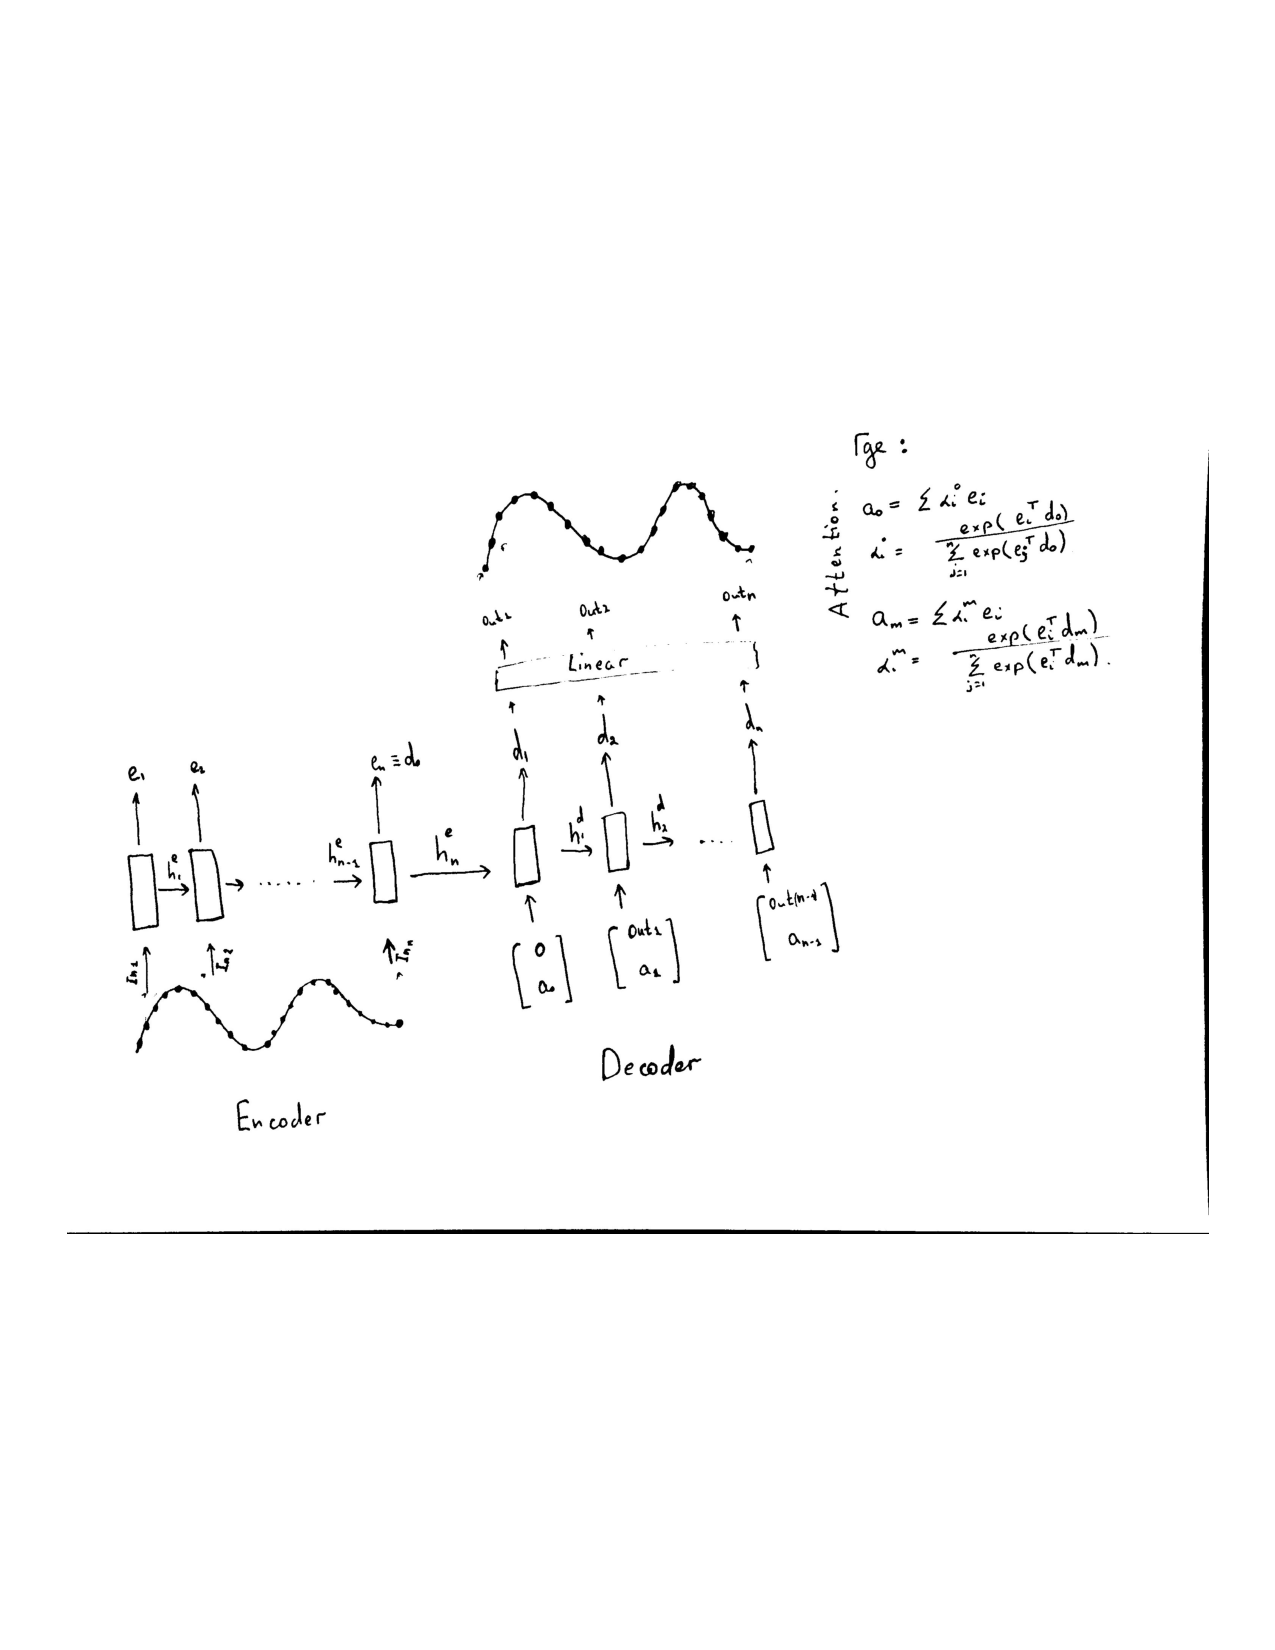
\includegraphics[width=0.5\textwidth]{figures/img1.pdf}\label{fig1}}
\subfloat[Описаниие предполагаемых результатов]{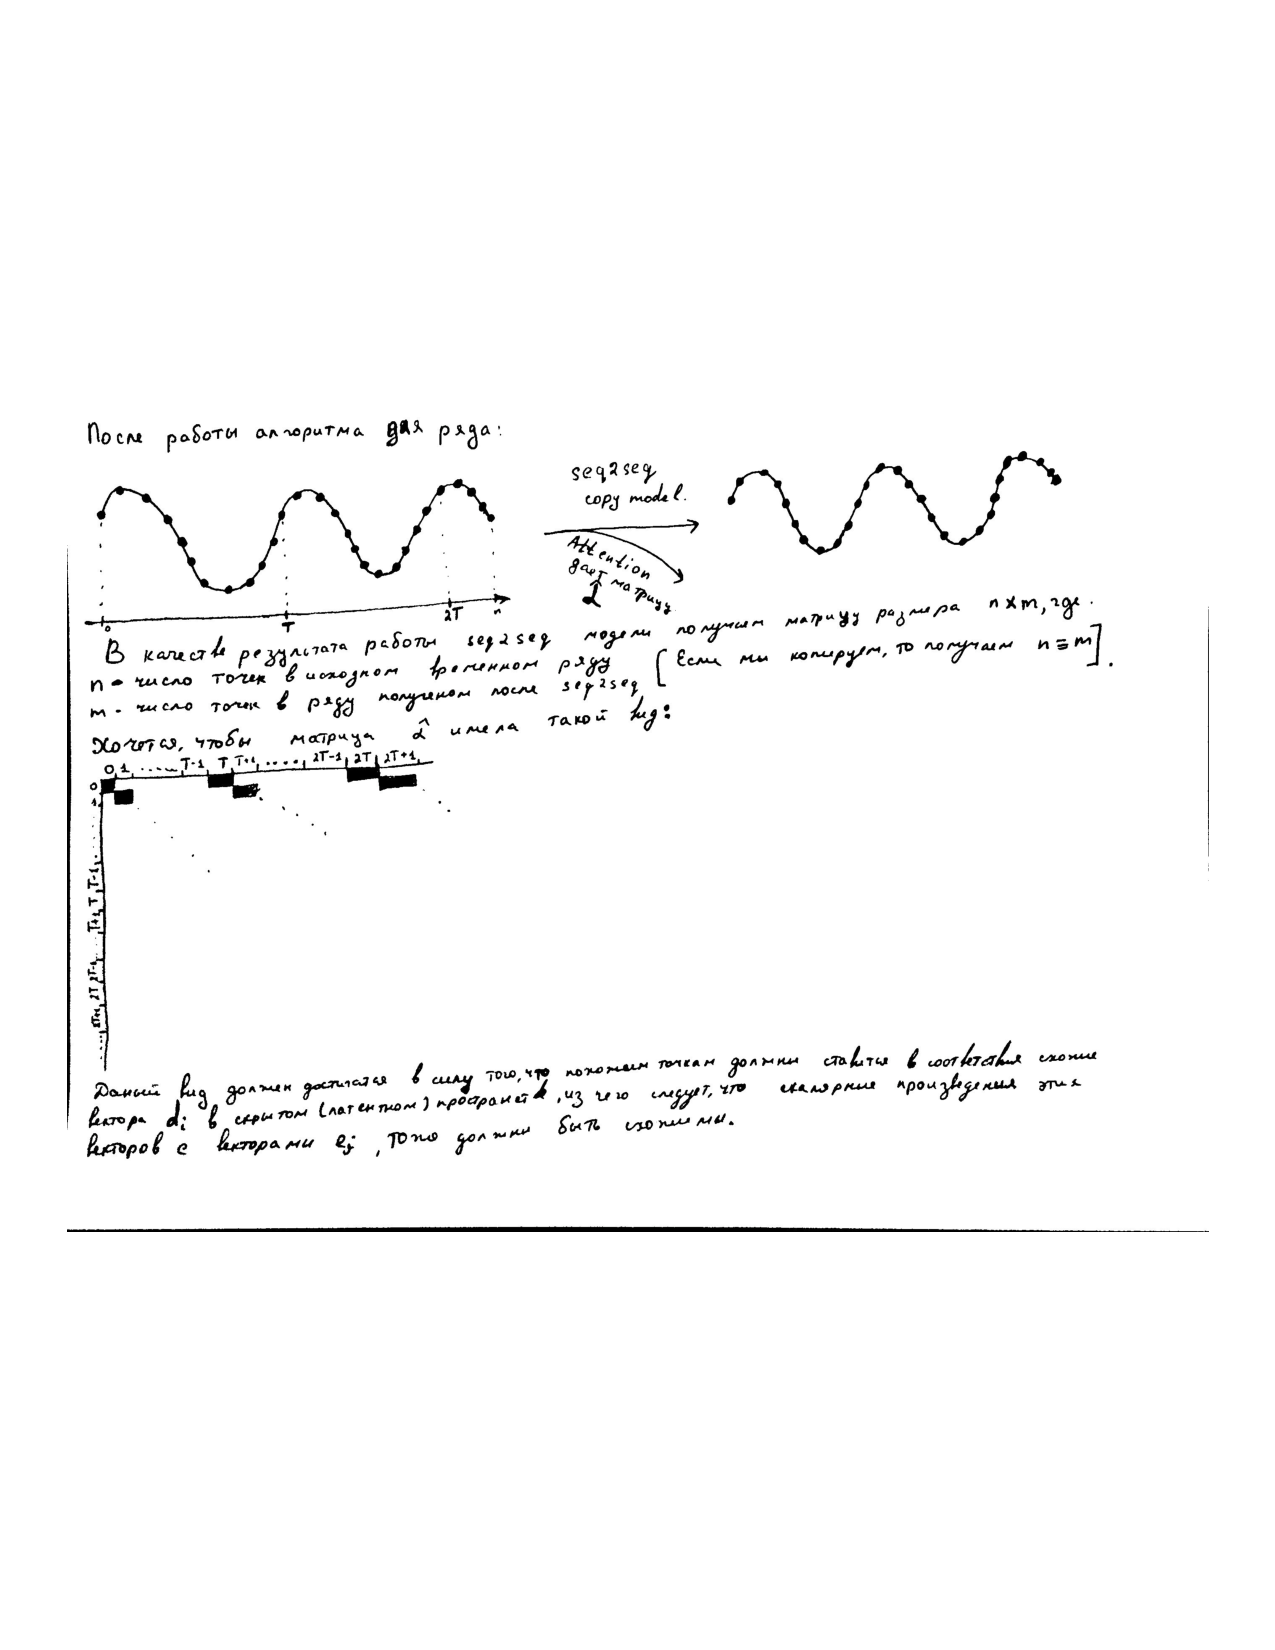
\includegraphics[width=0.5\textwidth]{figures/img2.pdf}\label{fig2}}
\caption{Основные сведения об seq2seq + Attention}
\end{figure}

Используем LSTM с простейшим Attention без дополнительных параметров. Пример, принцепа работы seq2seq c Attention показан на рис.~\ref{fig1}.

\section{Предположения}
Введя предположения о том, что скрытые вектора LSTM имеет похожие вектора для похожих кусков временного ряда можно предположить, что матрица Attention будет иметь вид показан на рис.~\ref{fig2}. Под матрицей Attention подрозумевается матрица размера $n\times m$, где $n, m$ --- длины входного и выходного сигналов соответственно, в ячейках которой показан уровень схожести (либо можно сказать уровень зависимости) между куском временного ряда на выходе и куском временного ряда на входе.

\section{Проблемы}
Предлагается использовать seq2seq, который просто копирует временной ряд. В этом методе есть ряд вопросов.
\begin{itemize}
    \item Первый косяк состоит в том, что если мы учим копировать временной ряд, и берем слишком сложный Attention с большим количеством параметров, то он начинает переобучатся, и в итоге получается матрица Attention диагональной. Это следует из того, что модель начинает просто учить друг за другом числа. Поэтому предлагается использовать просто скалярное произведение векторов (самую простую модель Attention, Dot метрика из~\ref{tab1}).
    
    \item Даже если взять простую модель Attention, все равно можно получить диагональную матрицу Attention, если мы просто будем копировать временной ряд, поэтому предлагается не просто учить все ряды из обучающего множества рядов, а на вход Encoder'а давать некоторый кусок (например из 100 сигналов ряда дать только первые 20 сигналов), и сравнивать как Decoder восстановит весь сигнал. Данный дополнительный финт немного улучшает качество.
    
    \item Второй вопрос состоит в том, что нужно придумать на каких данных учить данную модель (нужно подумать над тем какие сигналы давать на вход для копирования). Этот вопрос возникает в синтетических данных, но и в реальных данных. Я думаю, что можно модель учить не только на реальных данных, а и на синтетических, но для этого нужно придумать максимально правдоподобный сигнал акселерометра.
    
\end{itemize}

\begin{table}[h!]
\begin{center}
\caption{Описание разных Attention}
\label{tab1}
\begin{tabular}{|c|c|}
\hline
	Type & formula\\
	\hline
	Additive& $score_{i,j}~=~\textbf{w}_o\tanh\left(\textbf{W}_e\textbf{e}_i+\textbf{W}_d\textbf{d}_j\right)$\\
	\hline
	Dot& $score_{i,j}~=~\textbf{e}_i^{\mathsf{T}}\textbf{d}_j$\\
	\hline
	General& $score_{i,j}~=~\textbf{e}_i^{\mathsf{T}}\textbf{W}\textbf{d}_j$\\
\hline
\end{tabular}

\end{center}
\end{table}

\section{Эксперимент}
\subsection{Эксперимент с простыми периодическими структурами}

\begin{figure}[h!t]\center
\subfloat[$sin(x)$]{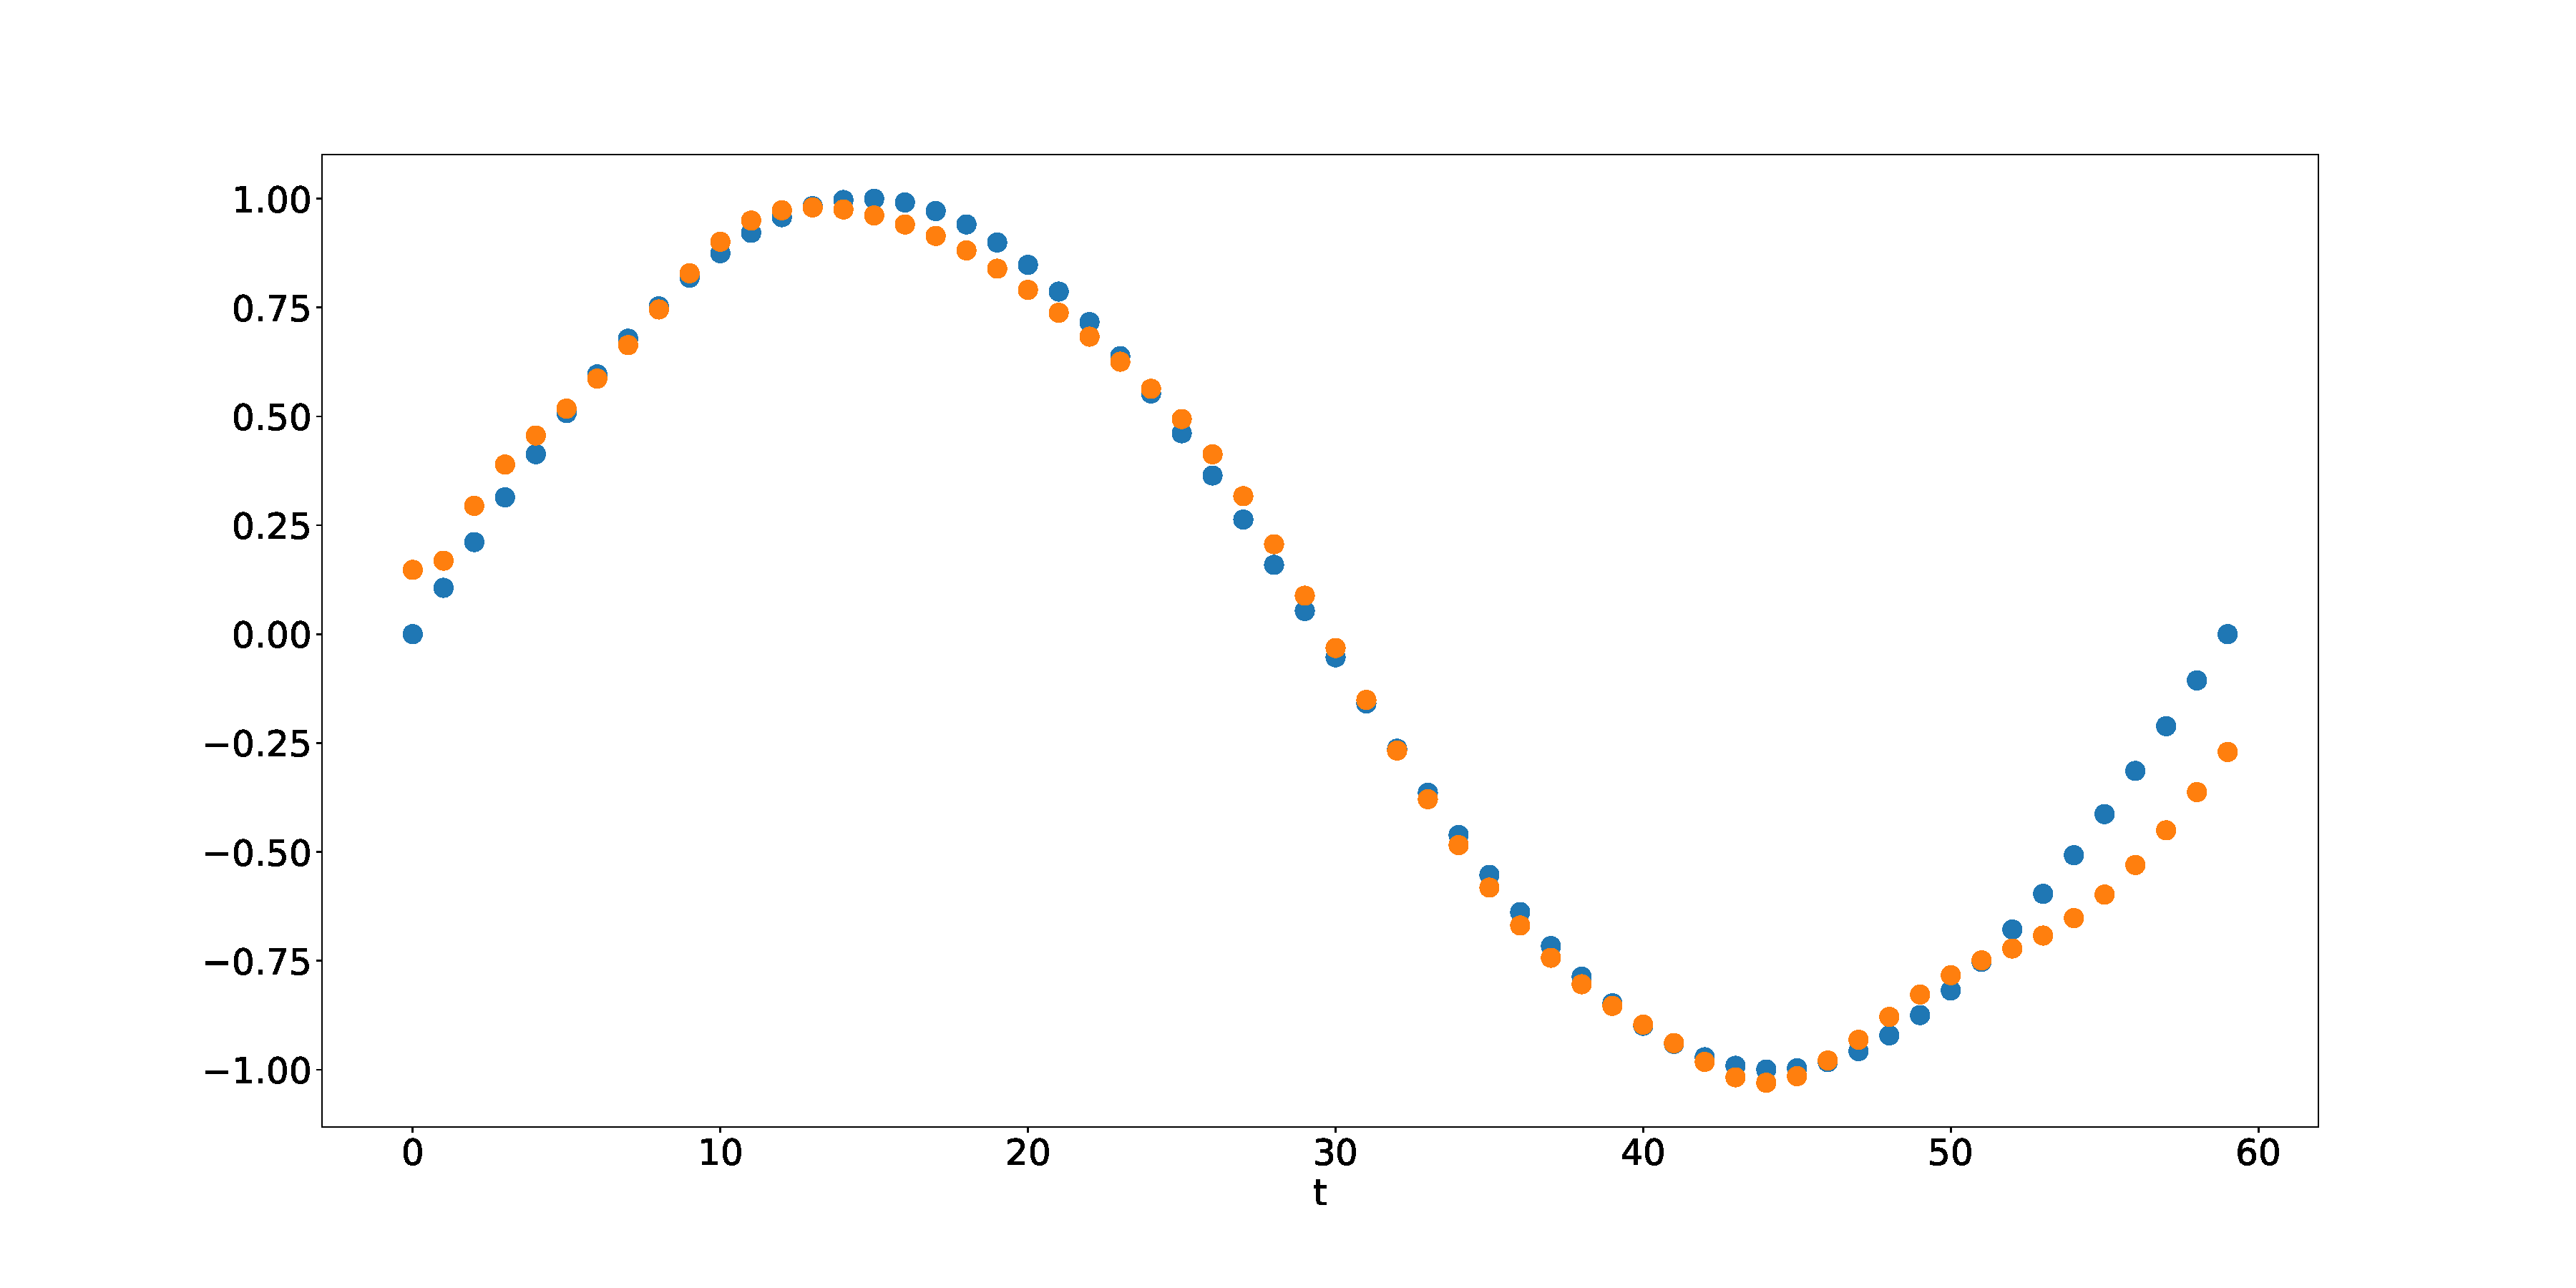
\includegraphics[width=0.5\textwidth]{figures/TimeSeries1.pdf}}
\subfloat[$sin(x)$]{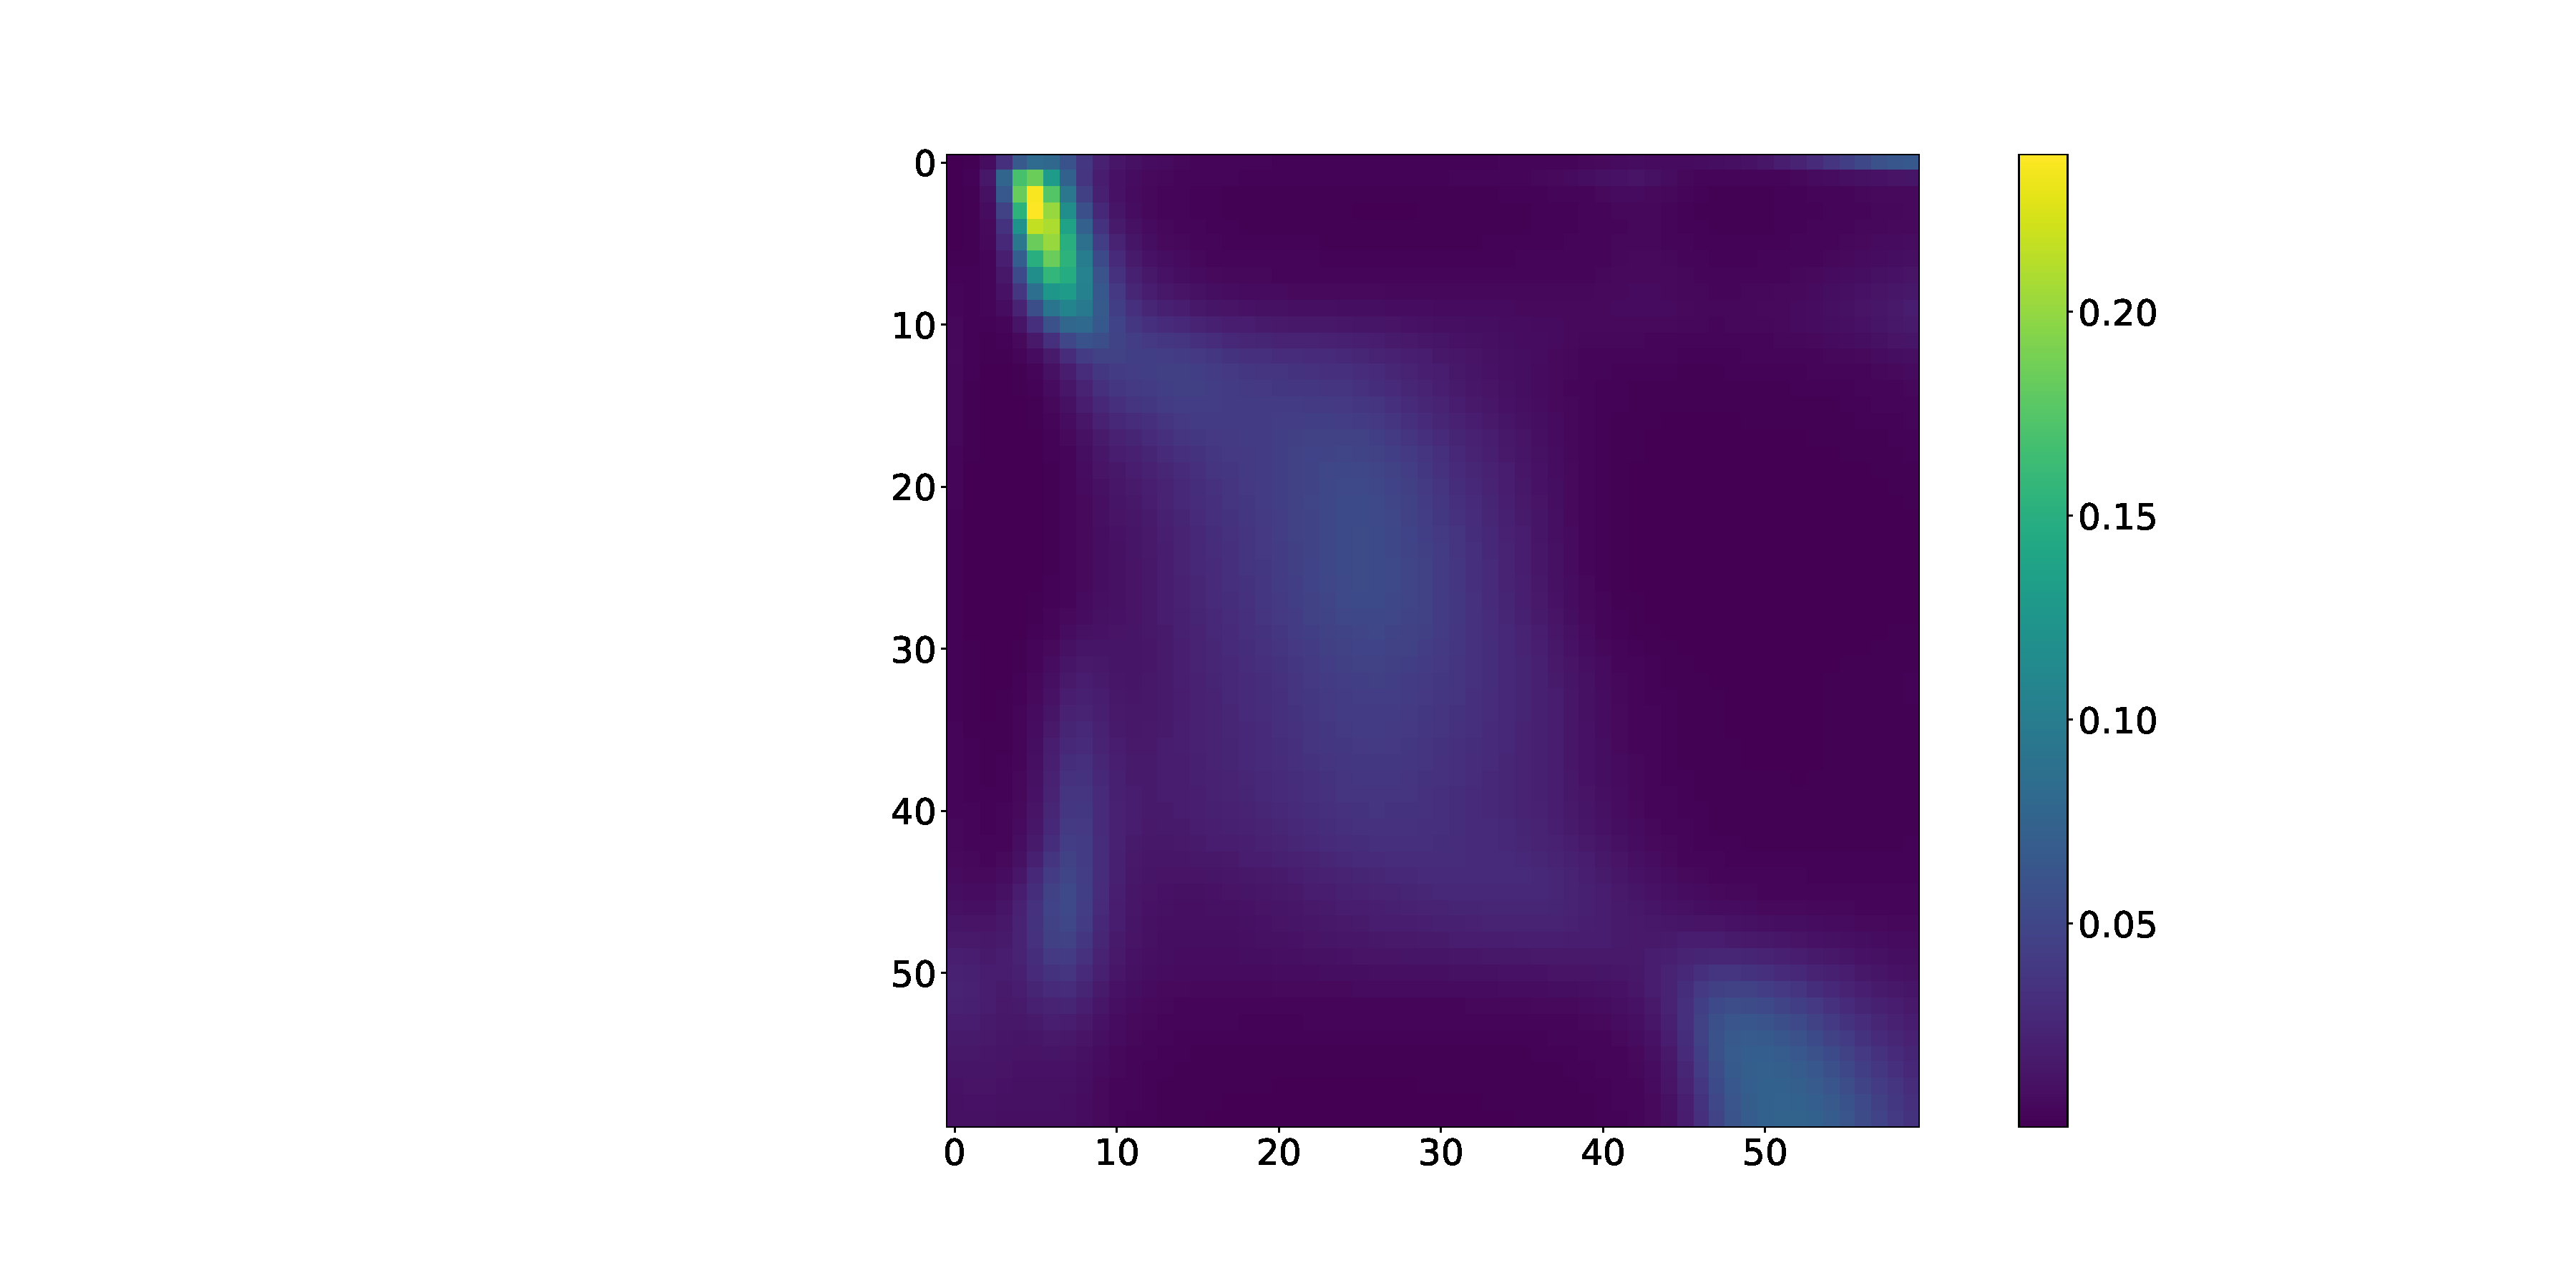
\includegraphics[width=0.5\textwidth]{figures/Attention1.pdf}}\\
\subfloat[$sin(2x)$]{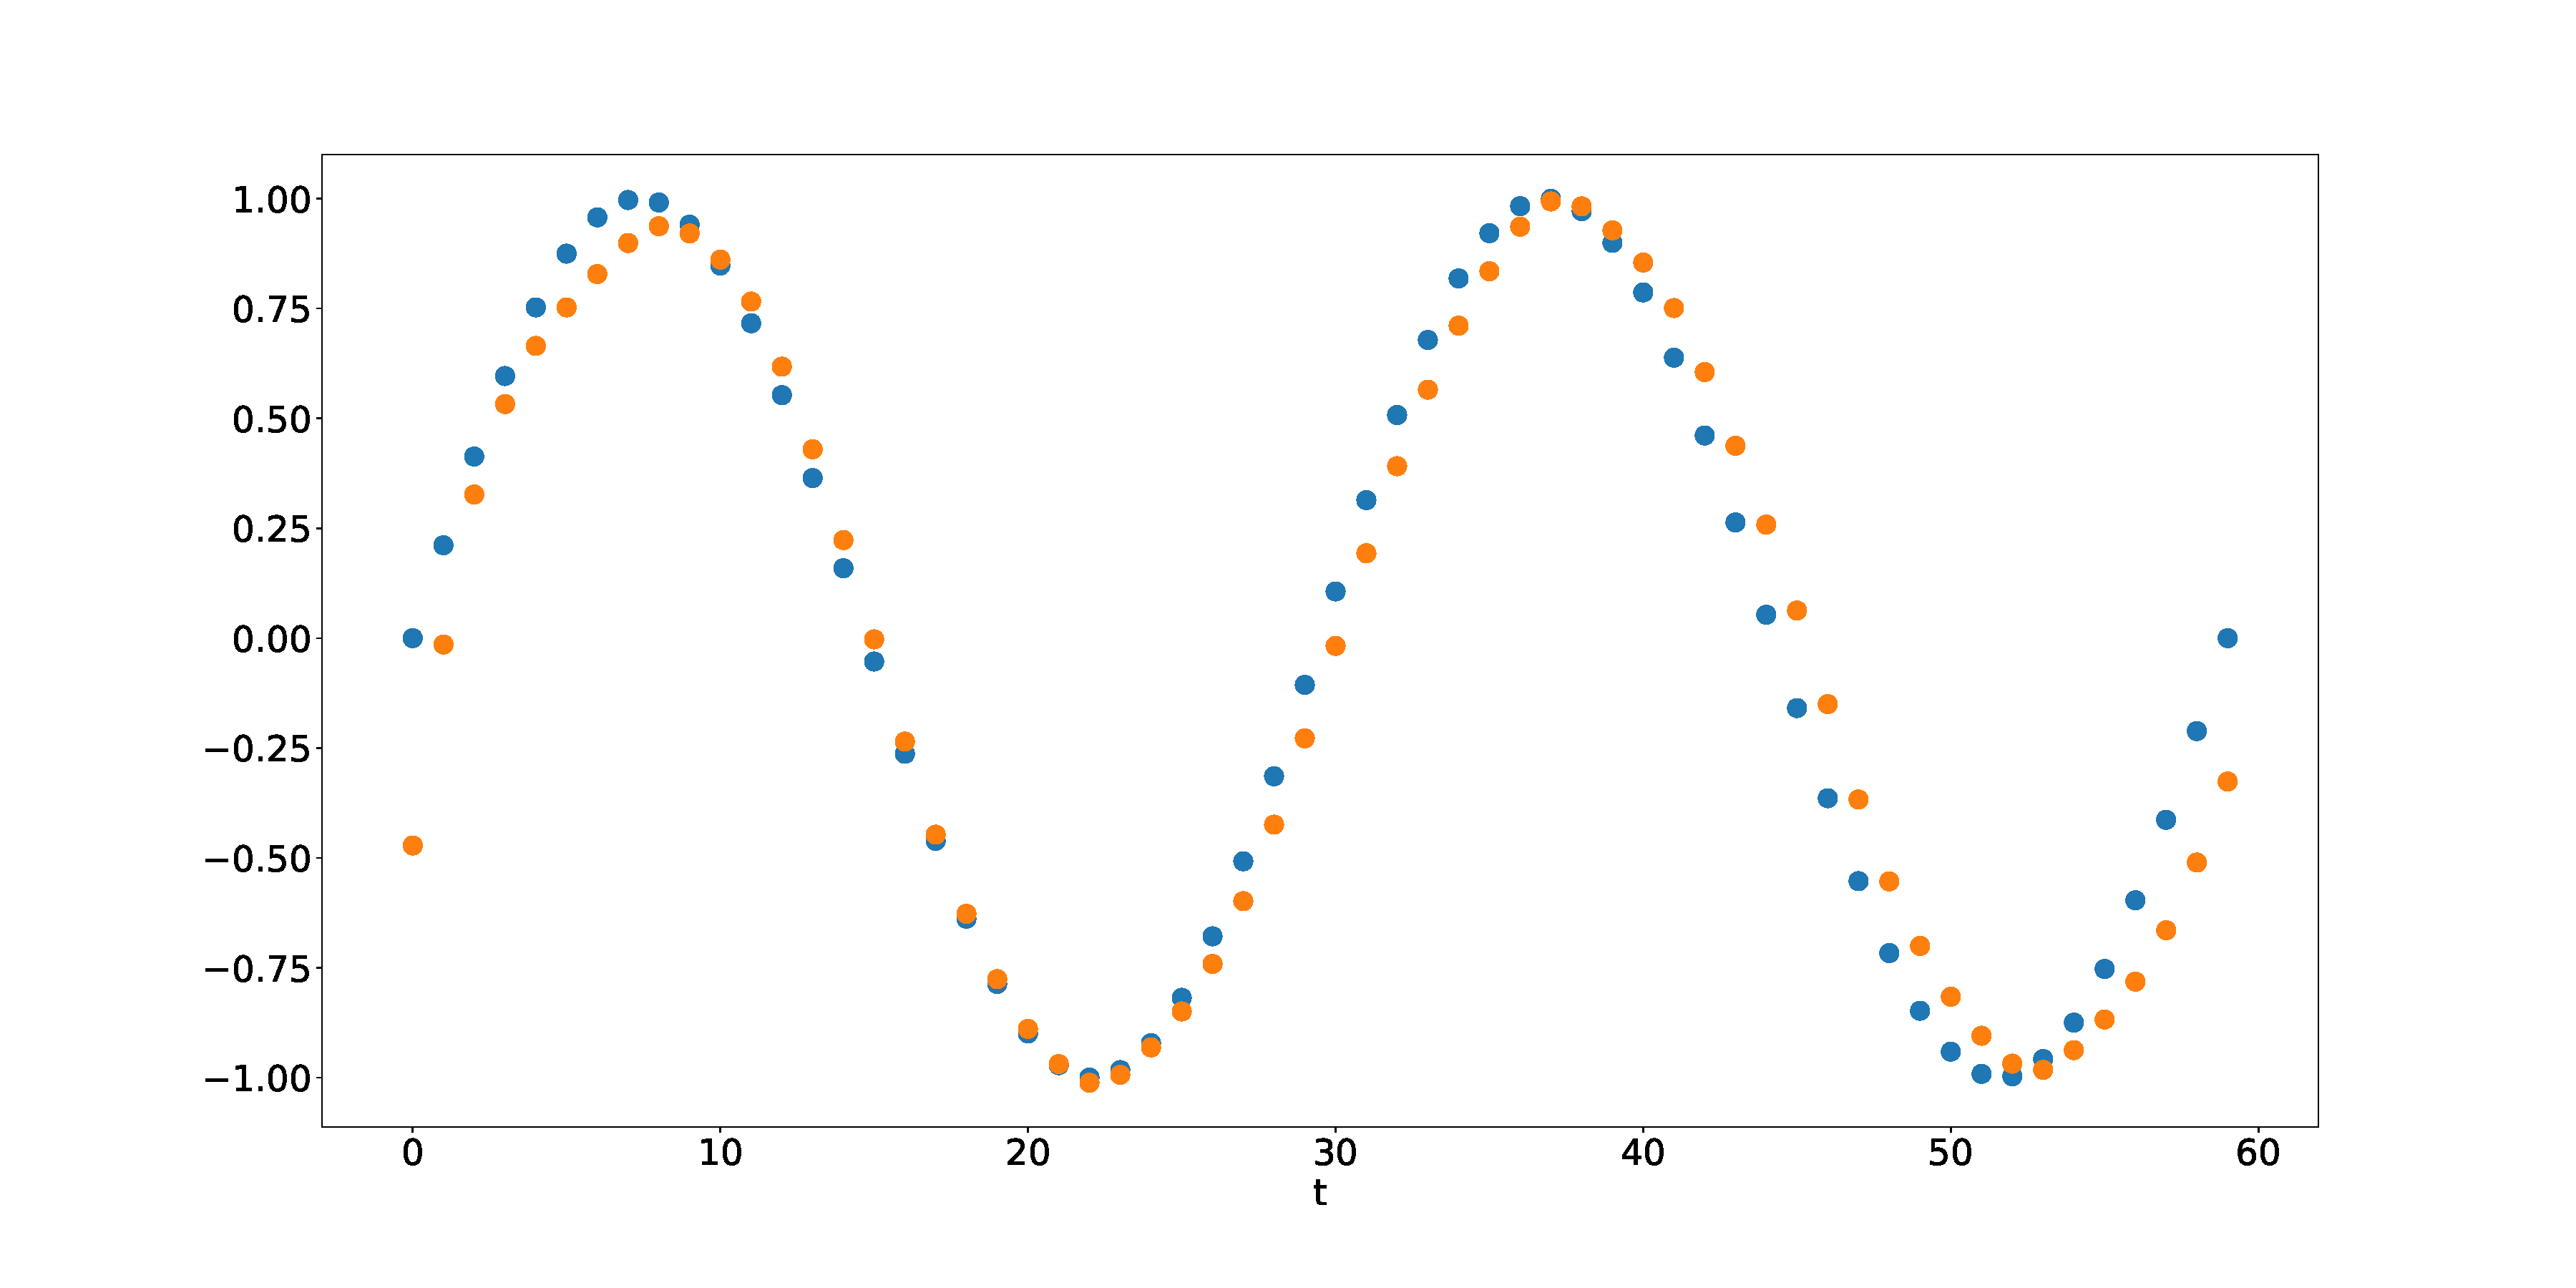
\includegraphics[width=0.5\textwidth]{figures/TimeSeries2.pdf}}
\subfloat[$sin(2x)$]{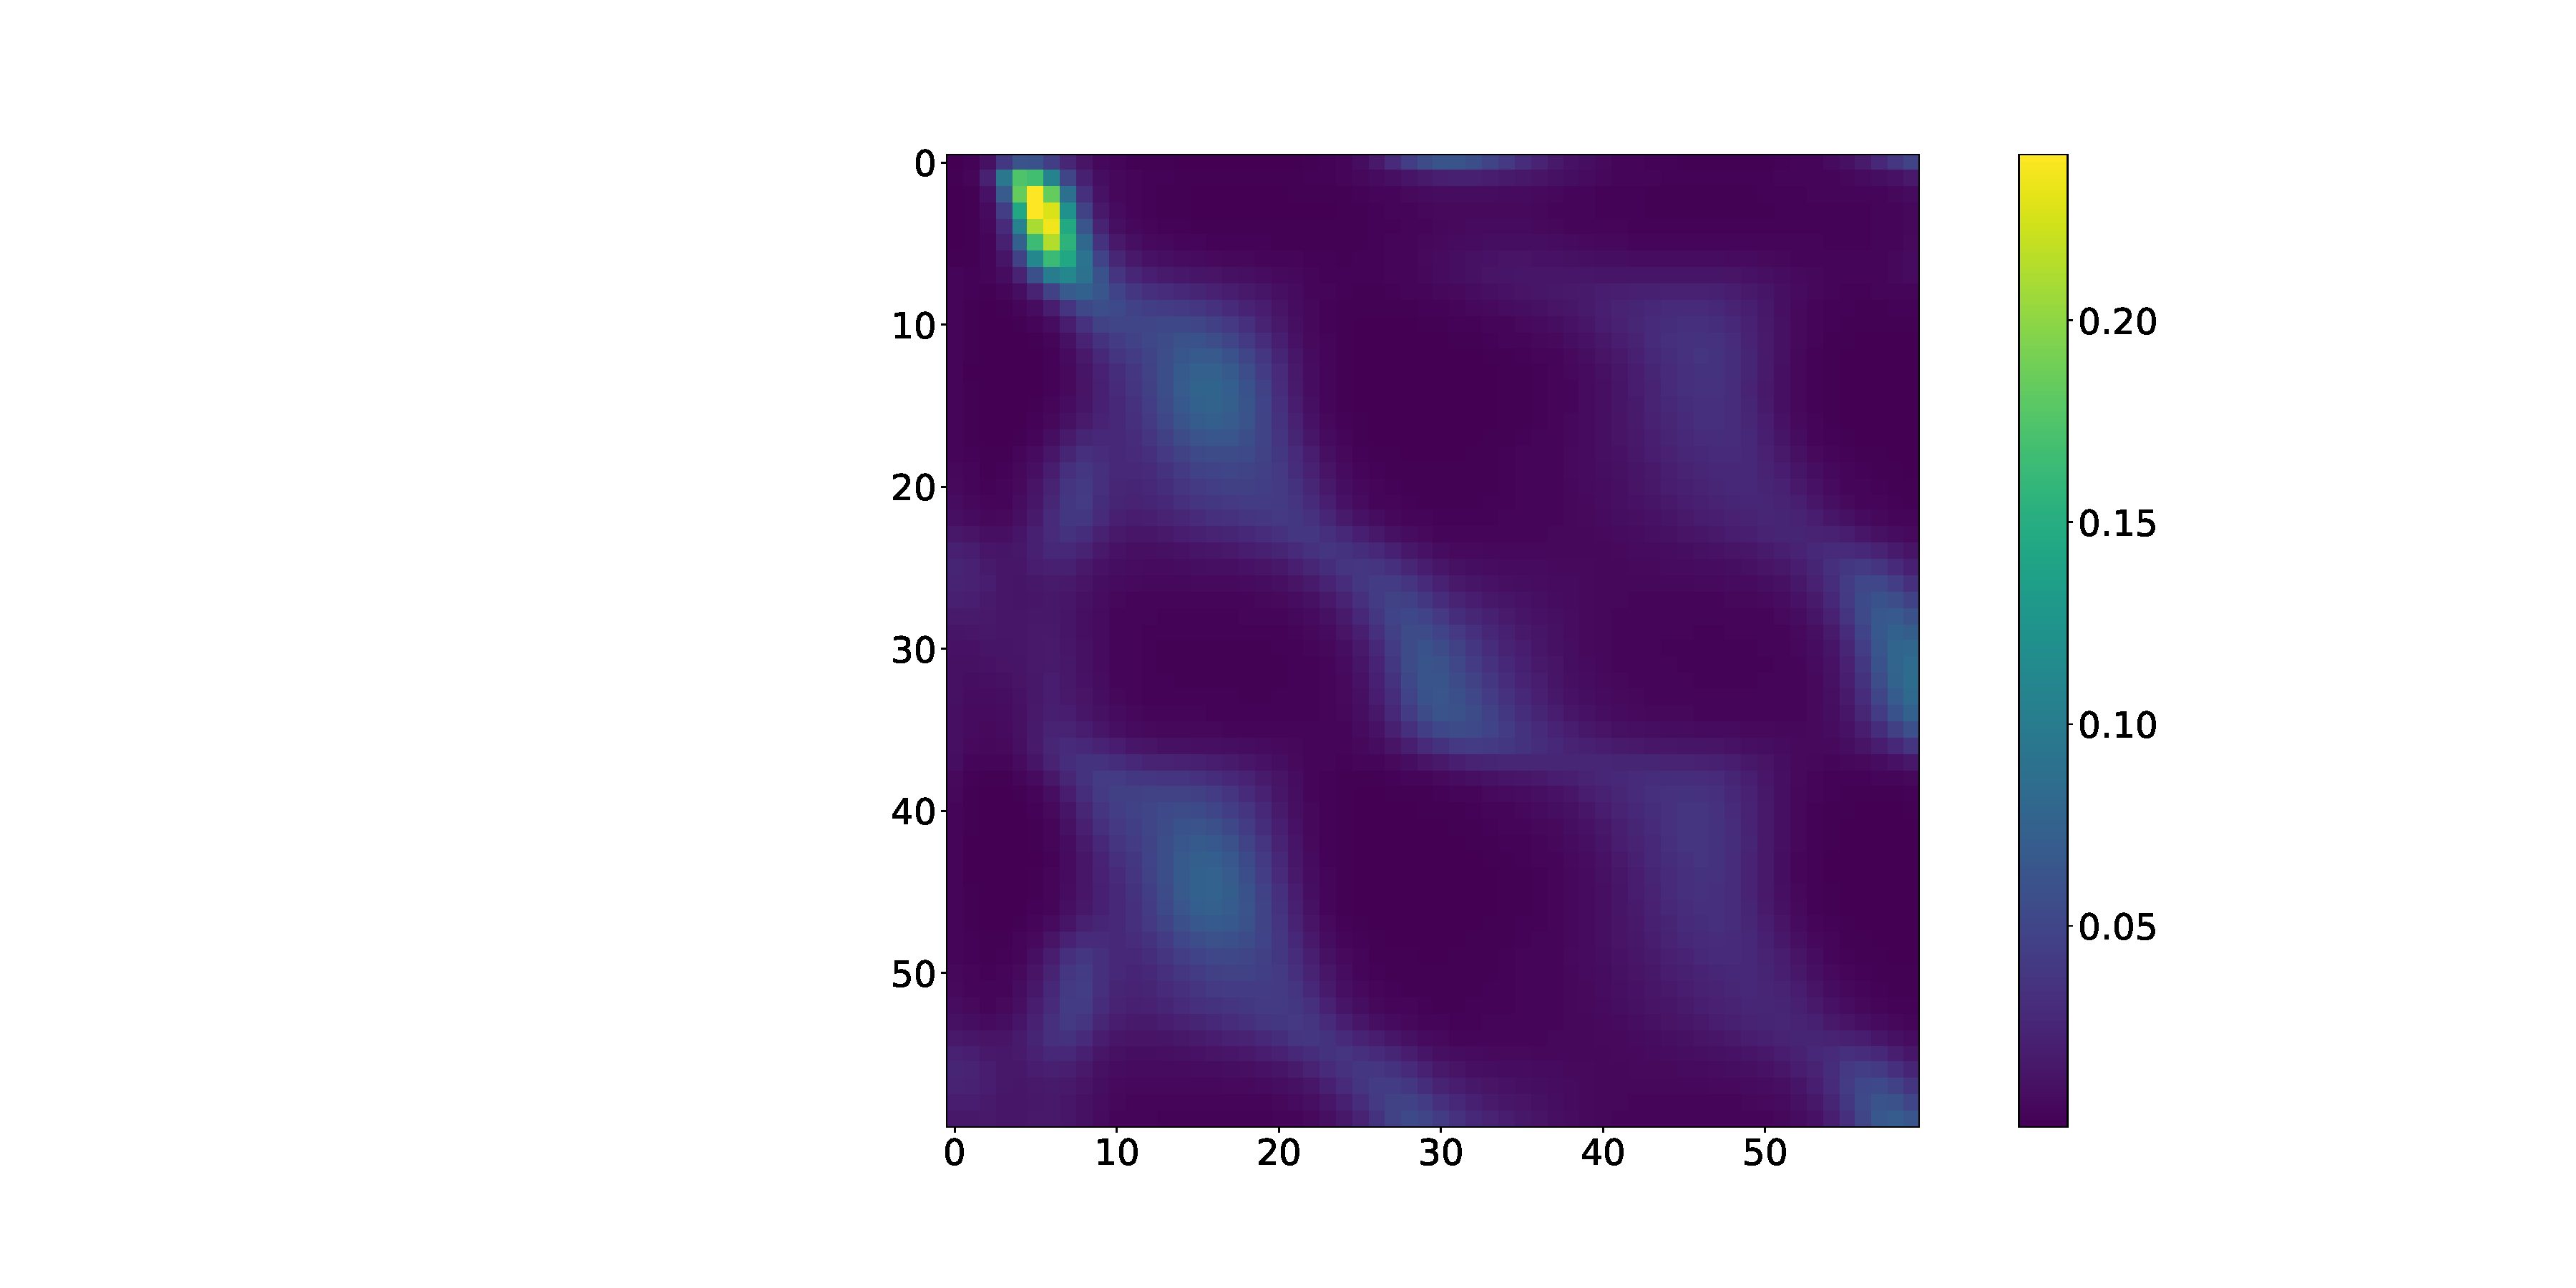
\includegraphics[width=0.5\textwidth]{figures/Attention2.pdf}}\\
\subfloat[$sin(8x)$]{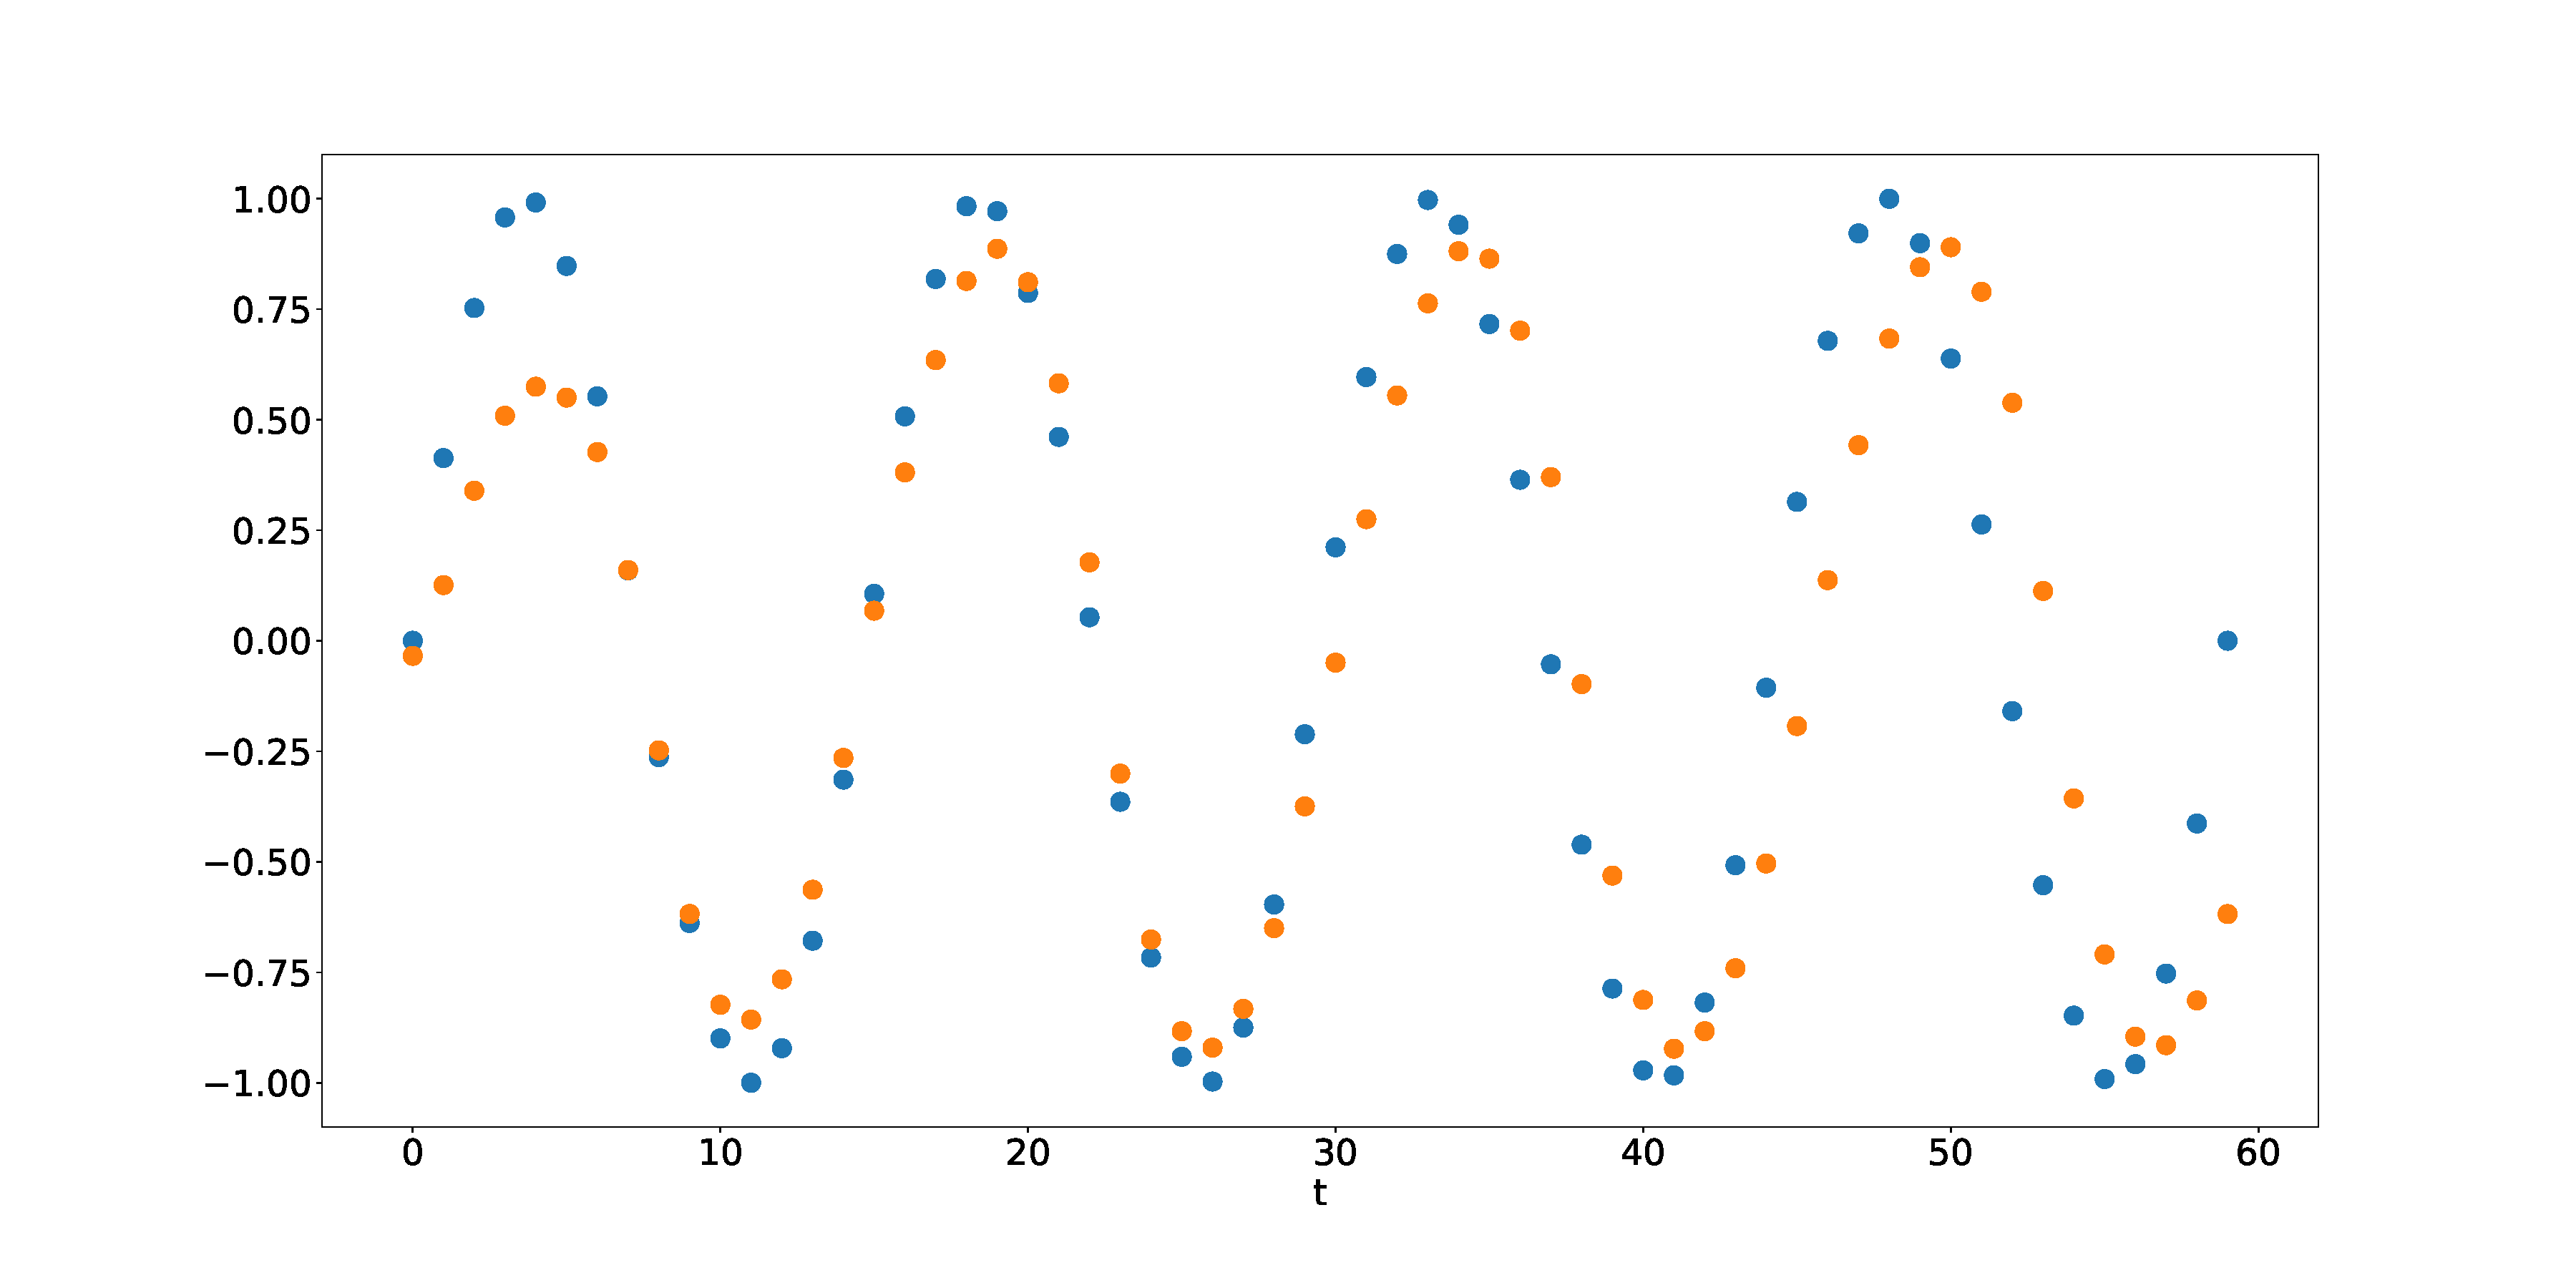
\includegraphics[width=0.5\textwidth]{figures/TimeSeries3.pdf}}
\subfloat[$sin(8x)$]{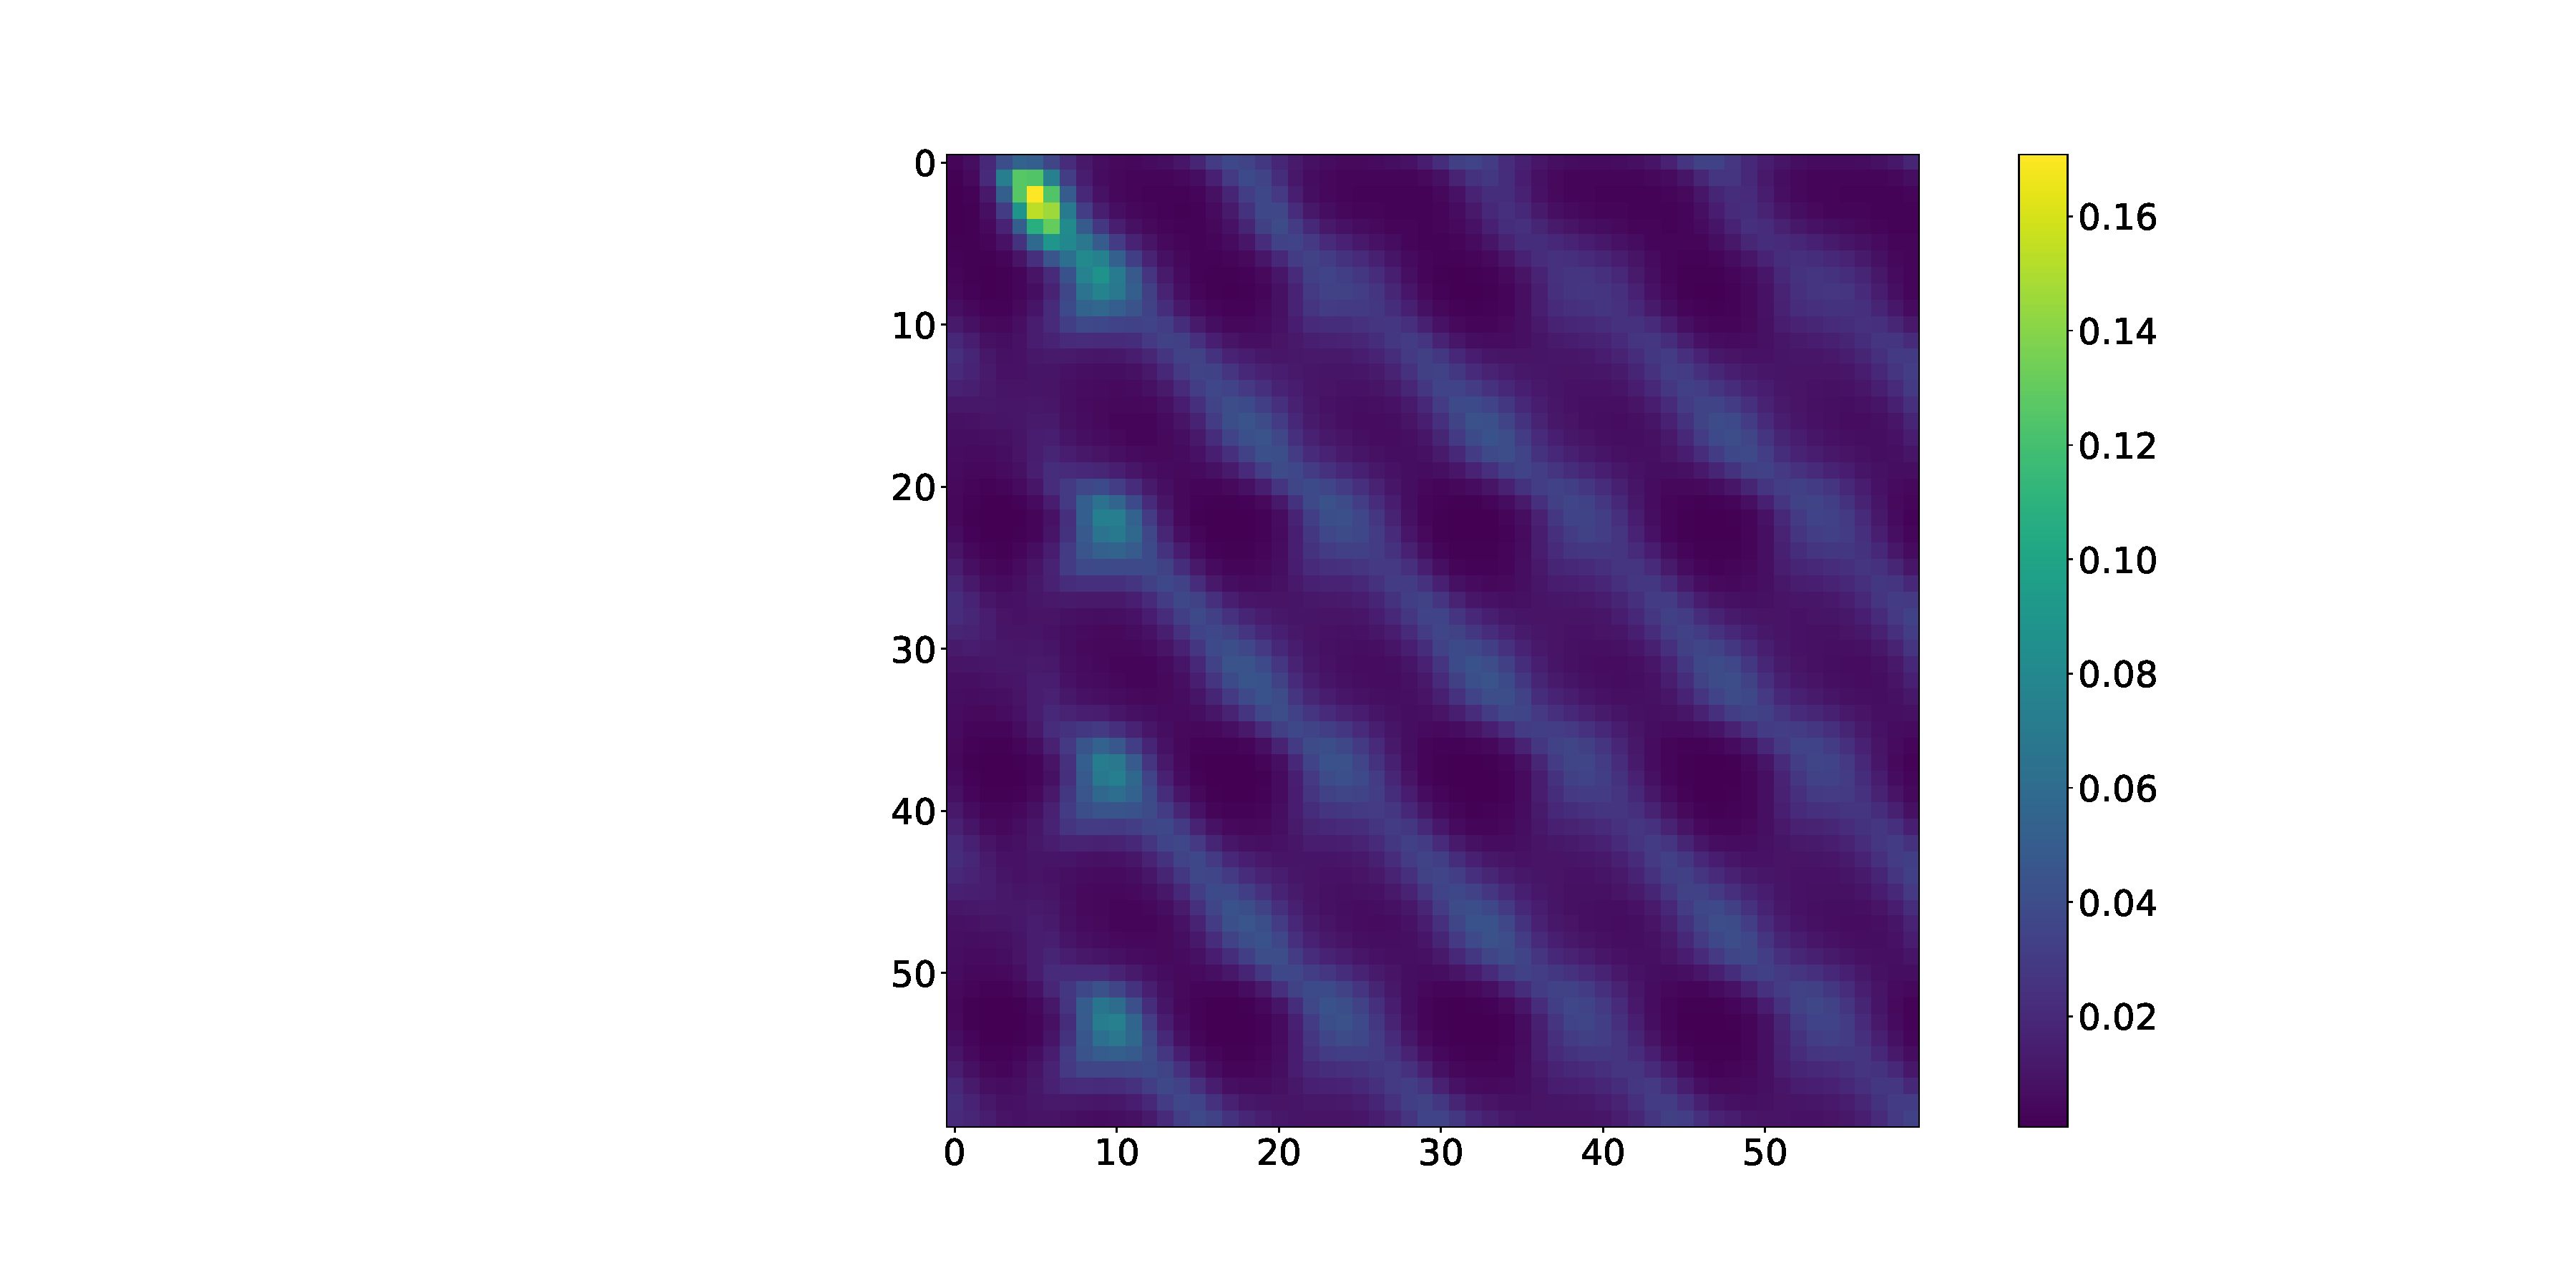
\includegraphics[width=0.5\textwidth]{figures/Attention3.pdf}}\\

\caption{Результаты для модели с рис.~\ref{fig1}}
\label{fig3}
\end{figure}



Пусть модель обучена на синусоидальных сигналах с произвольной частотой, произвольной амплитудой и произвольной начальной фазой. Как видно из результатов на рис.~\ref{fig3}, предположение о виде матрицы Attention подтверждается. На рис~\ref{fig3} показано как меняется вид матрицы Attention в зависимости от частоты синуса. Видно что количество диагоналей в матрице Attention соответствует частоте синусоидального сигнала.

В работе~\cite{cinar2018} показано, что для нахождения периодов во временном ряде нельзя использовать простой Attention. Был пердложен модифицированный Attention который виглядит в следующем виде:

$$e_{ij}=~=~\textbf{w}_o\tanh\left(\textbf{W}_e\left(\bm{\pi}_{i-j}\textbf{e}_i\right)+\textbf{W}_d\textbf{d}_j\right)\cdot \left[i-j \leq T\right], \eqno(1)$$
где $\bm{\pi}$ --- еще один обучаемый вектор параметров, который указывает на степень зависимости $i$-го и $j$-го элемента.
	
Мои эксперименты показали, что прирост качества в двух разных Attention не очень большой, поэтому можно использовать любой из них.


\subsection{Эксперимент с простыми переодическими структурами в случае размерности скрытого пространства $2$}


\begin{figure}[h!t]\center
\subfloat[]{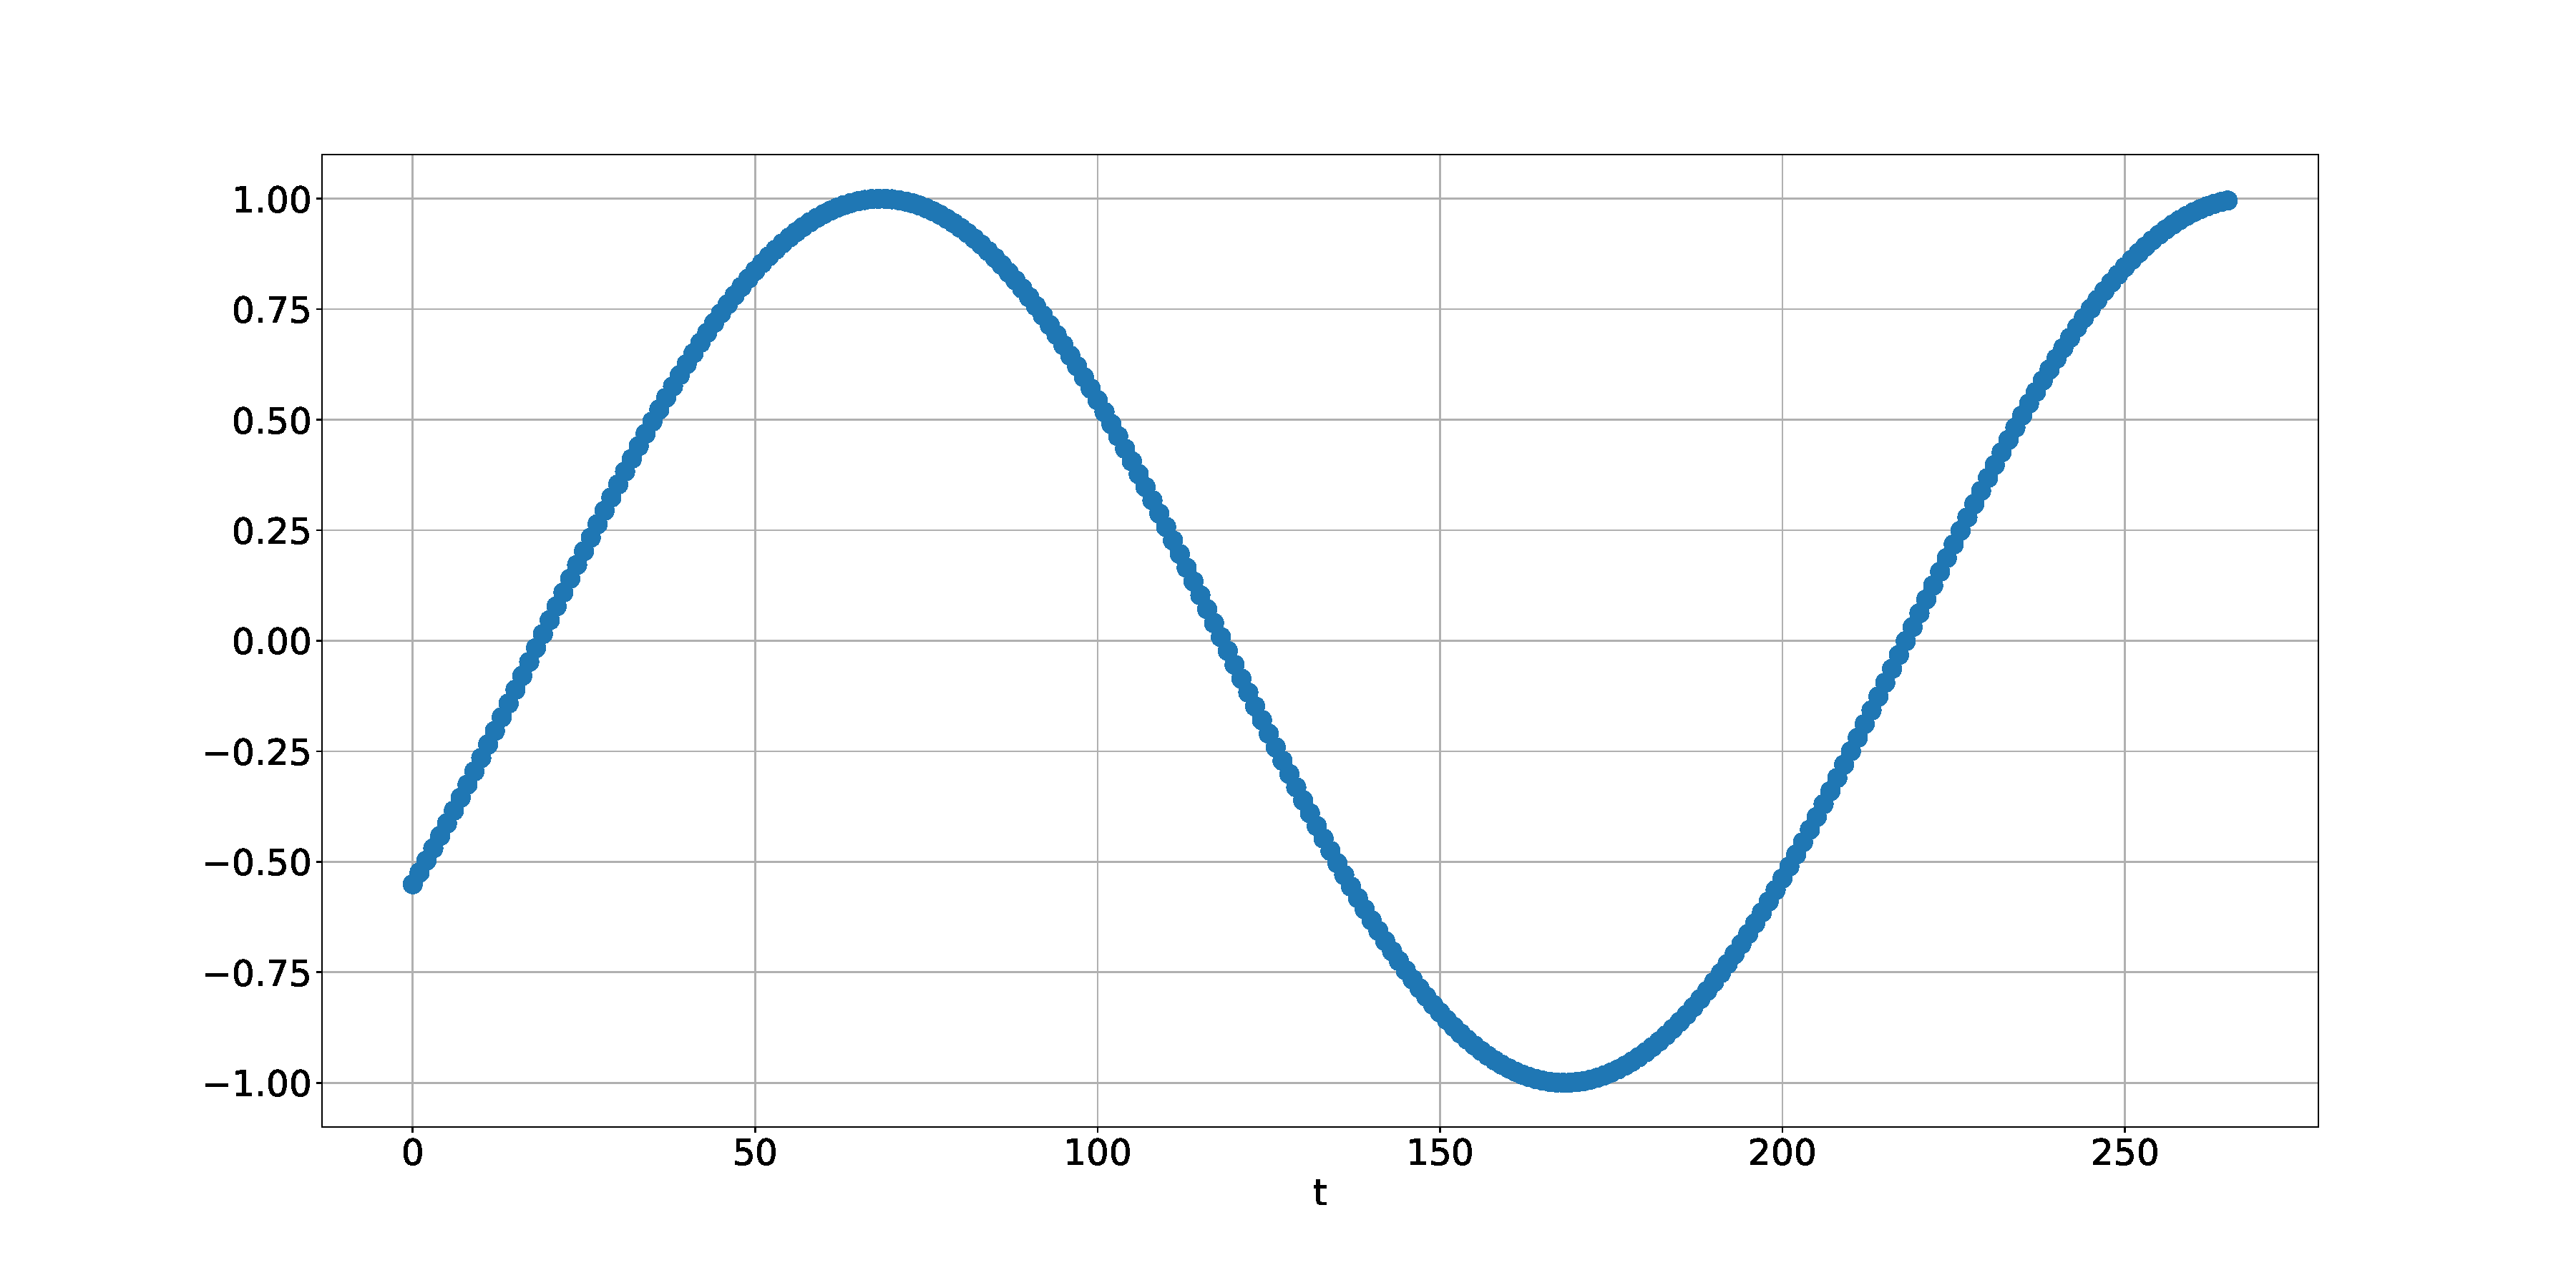
\includegraphics[width=0.5\textwidth]{figures/TimeSeries1_2dim.pdf}}
\subfloat[]{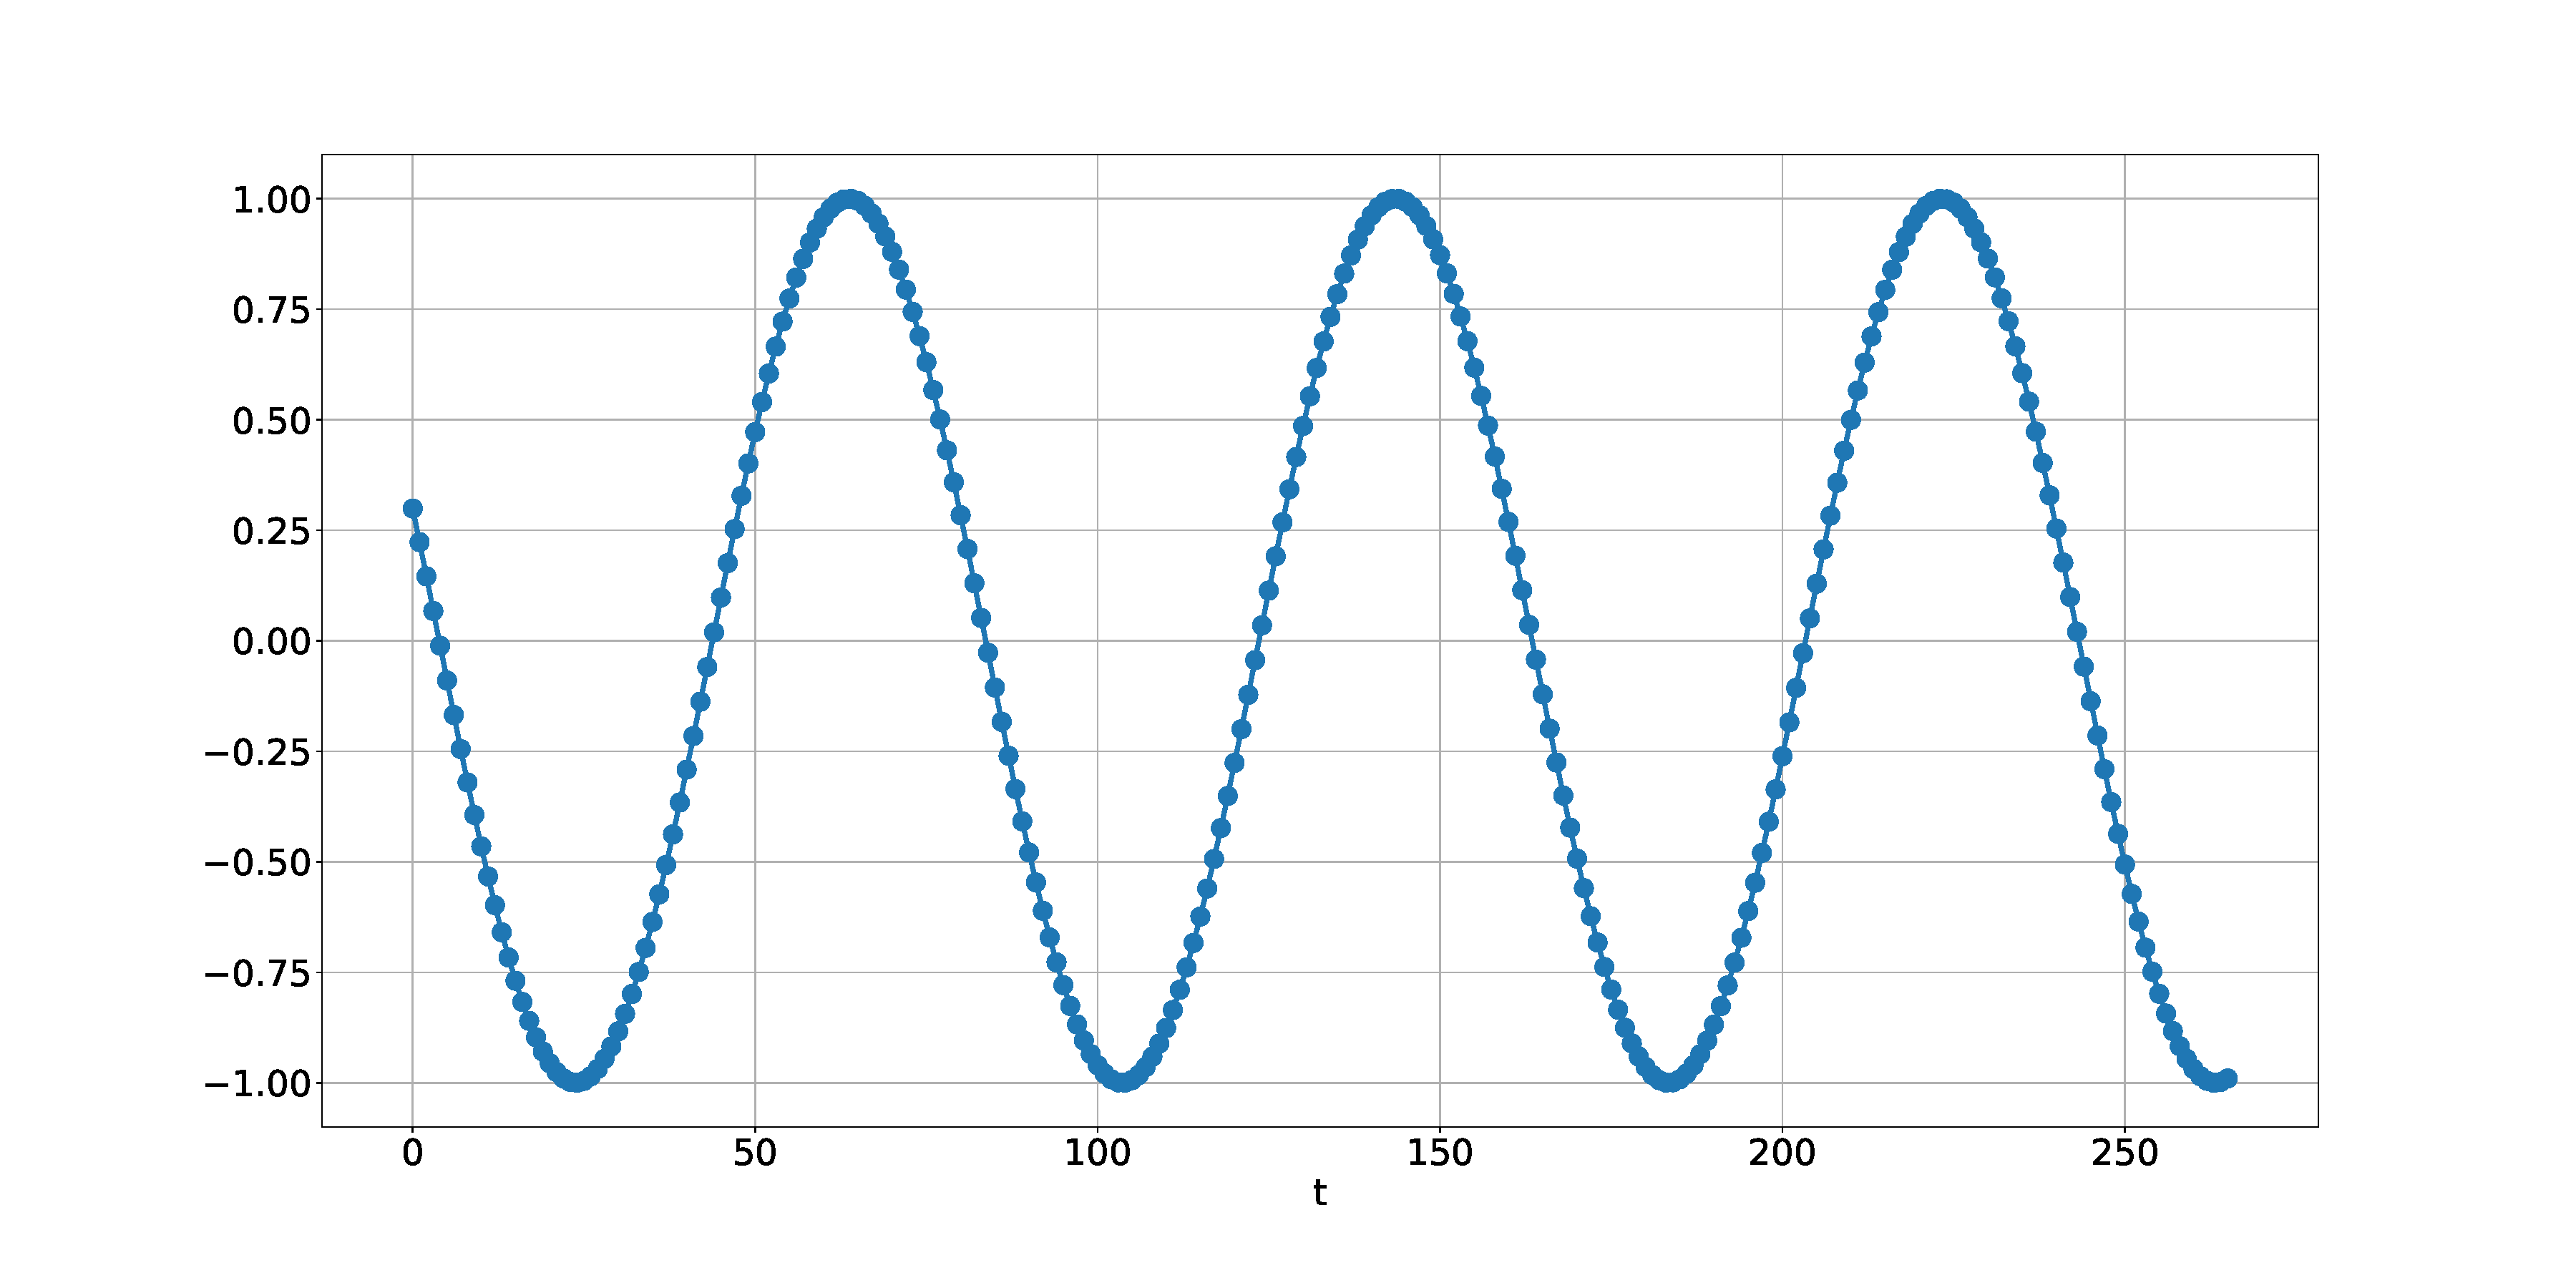
\includegraphics[width=0.5\textwidth]{figures/TimeSeries2_2dim.pdf}}\\
\subfloat[]{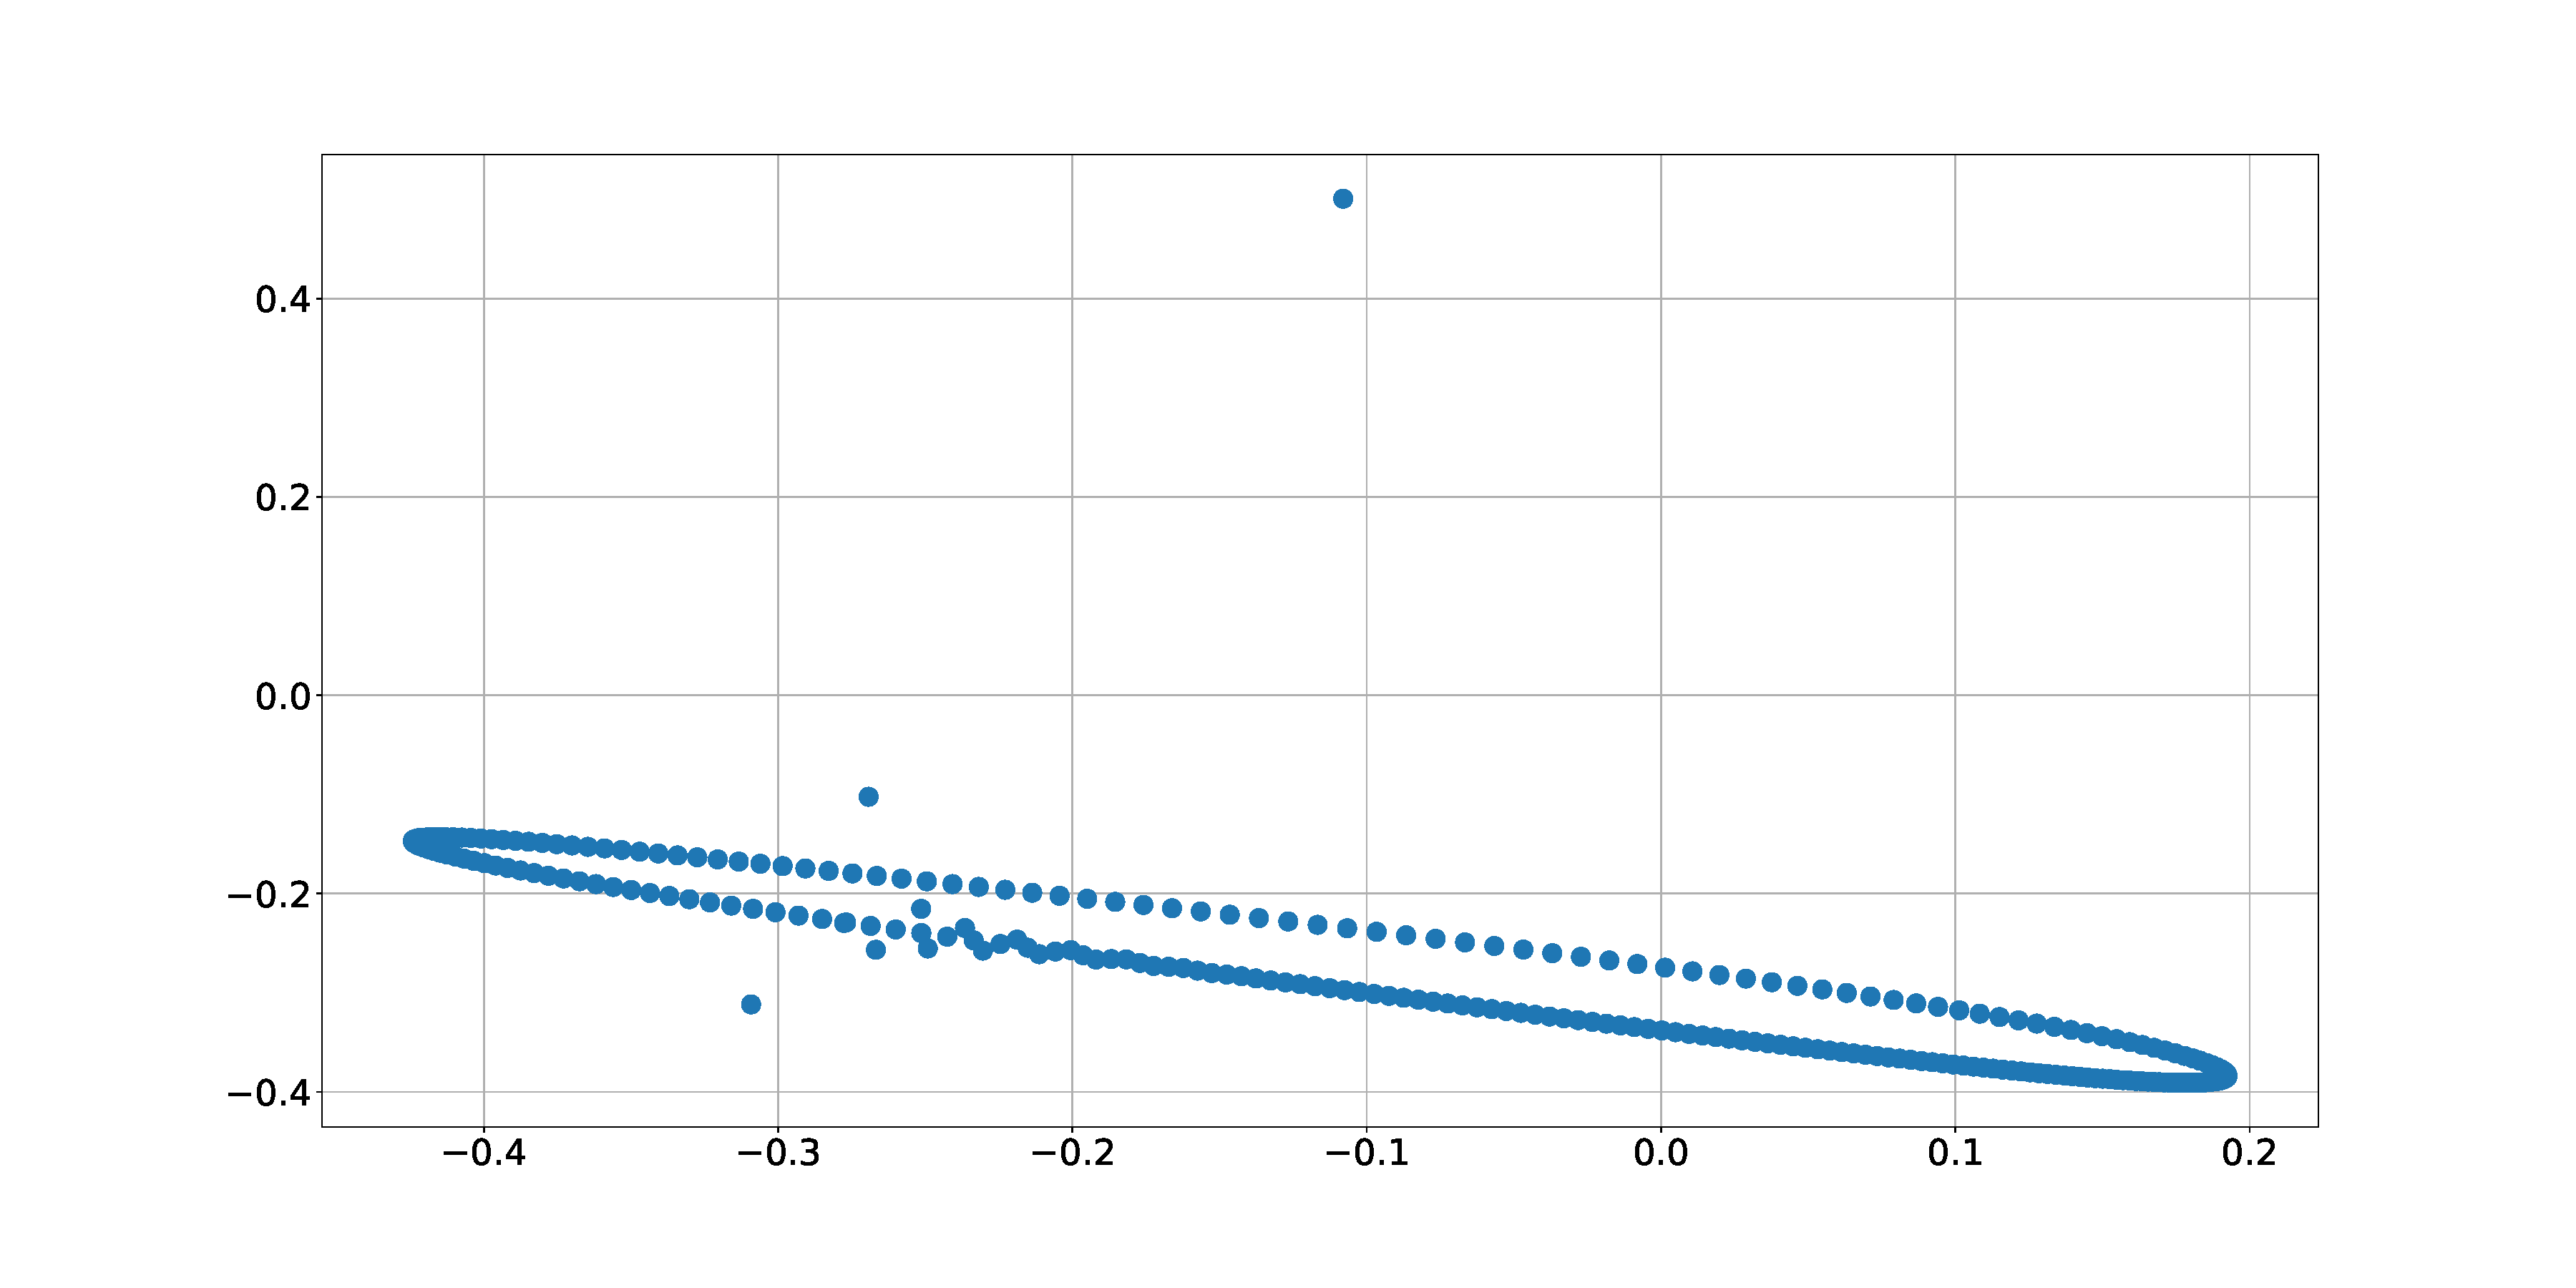
\includegraphics[width=0.5\textwidth]{figures/hidden1_2dim.pdf}}
\subfloat[]{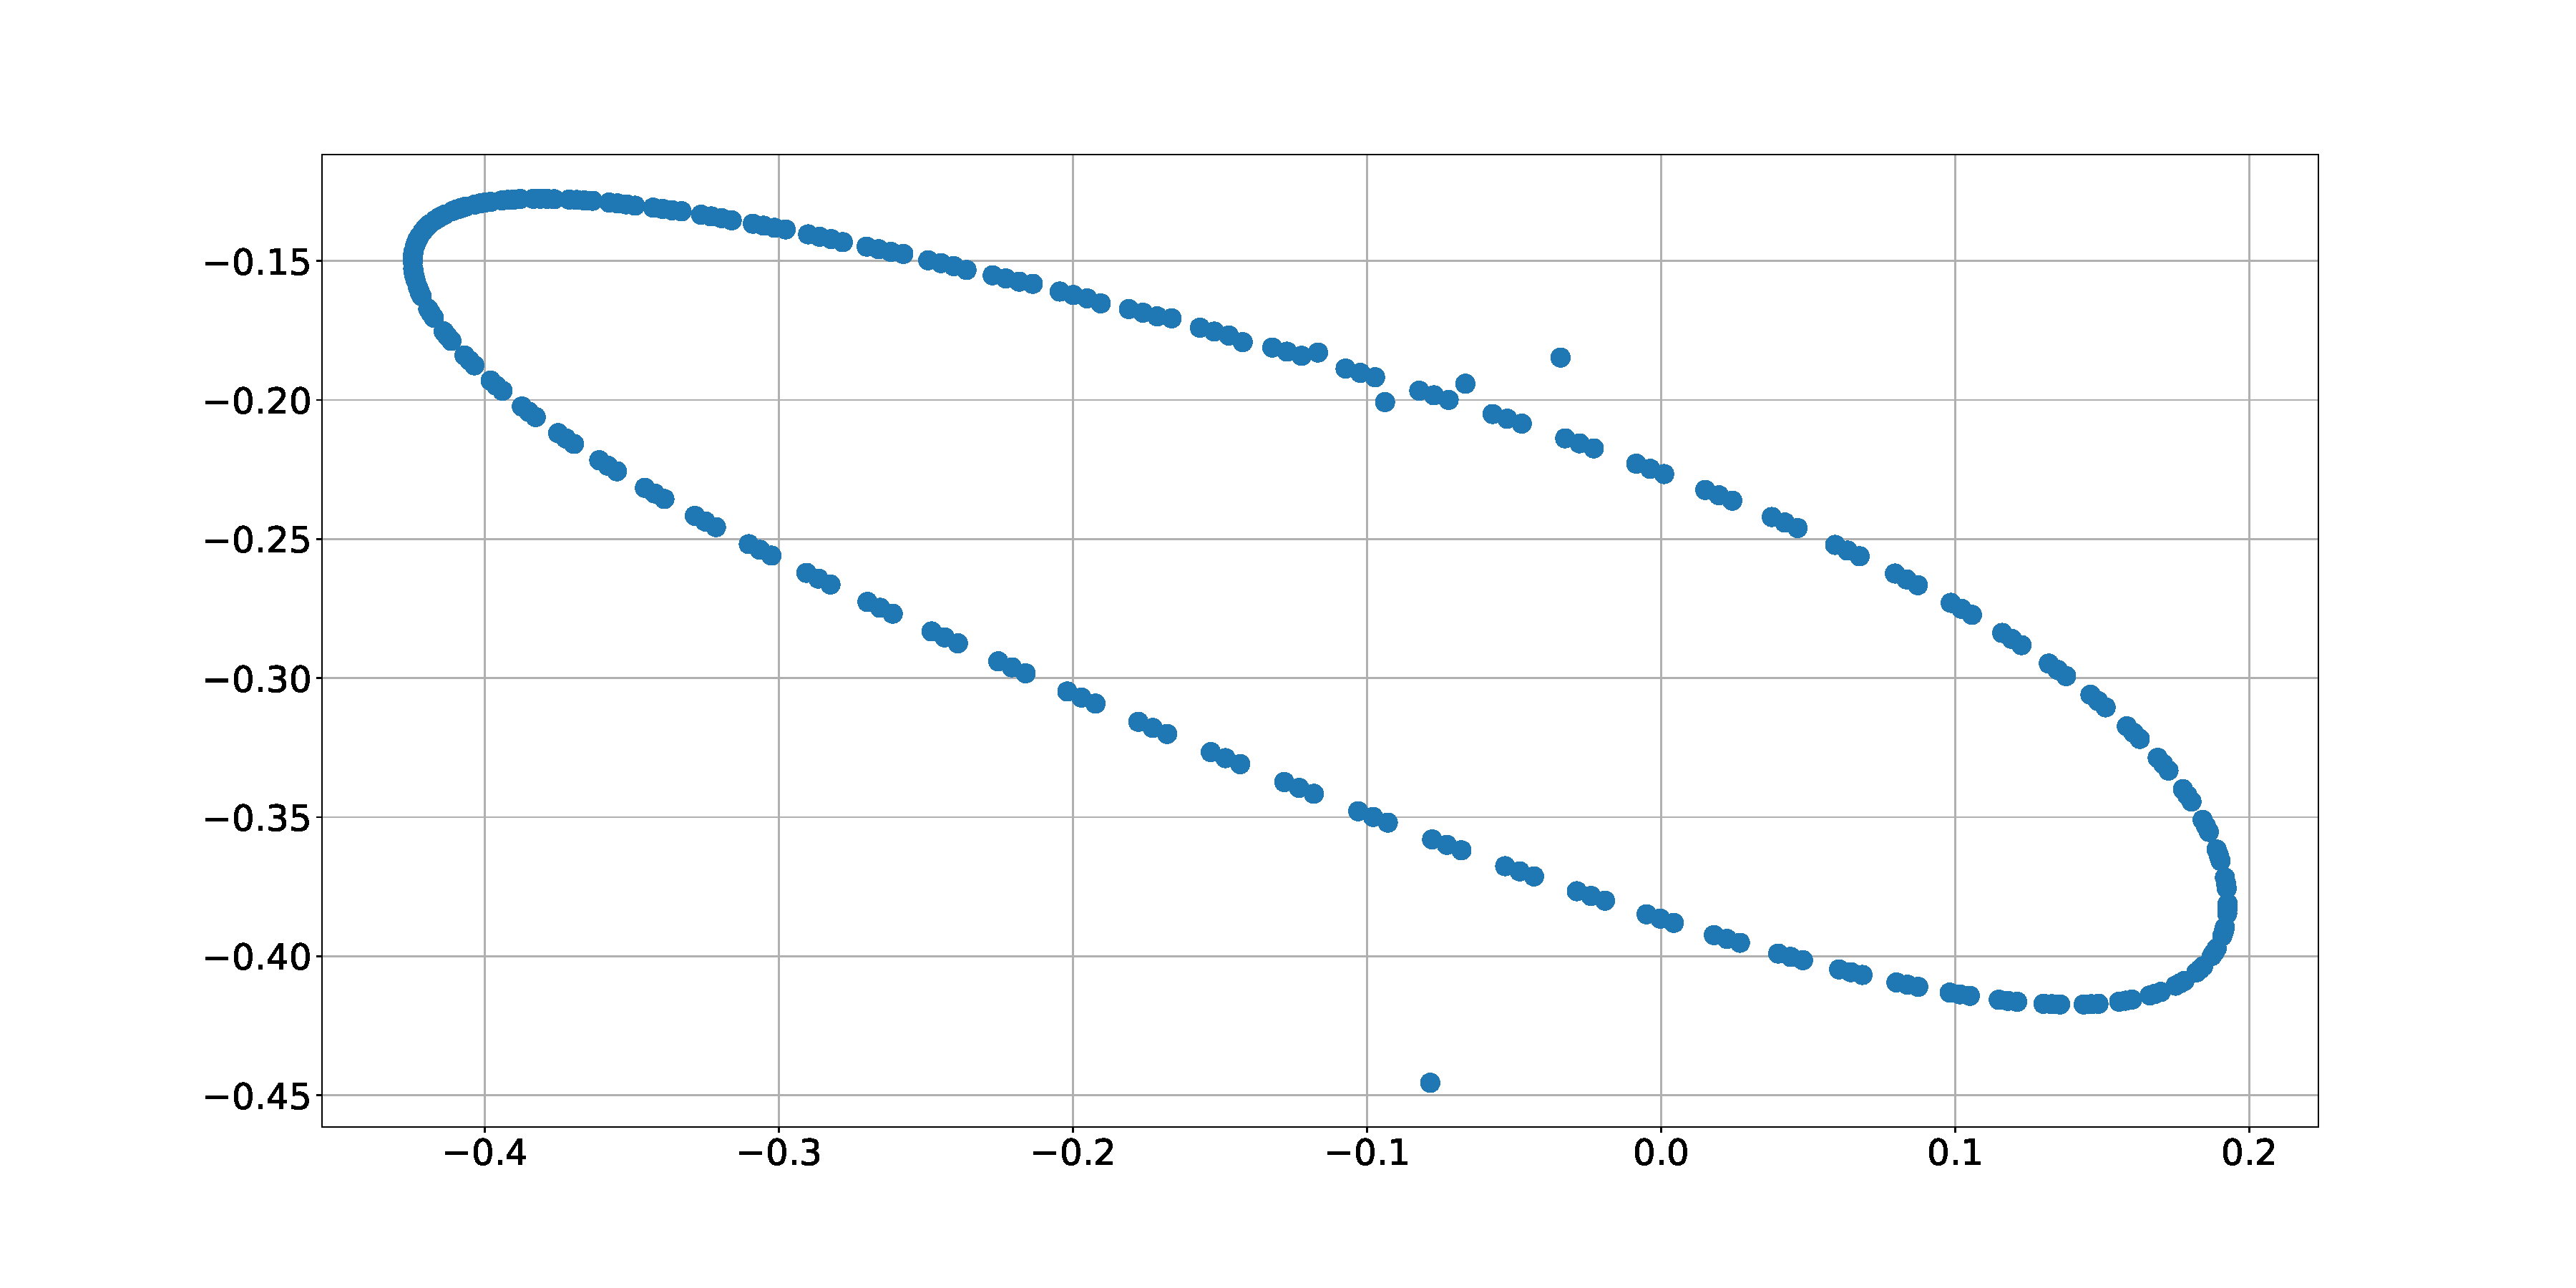
\includegraphics[width=0.5\textwidth]{figures/hidden2_2dim.pdf}}\\
\subfloat[]{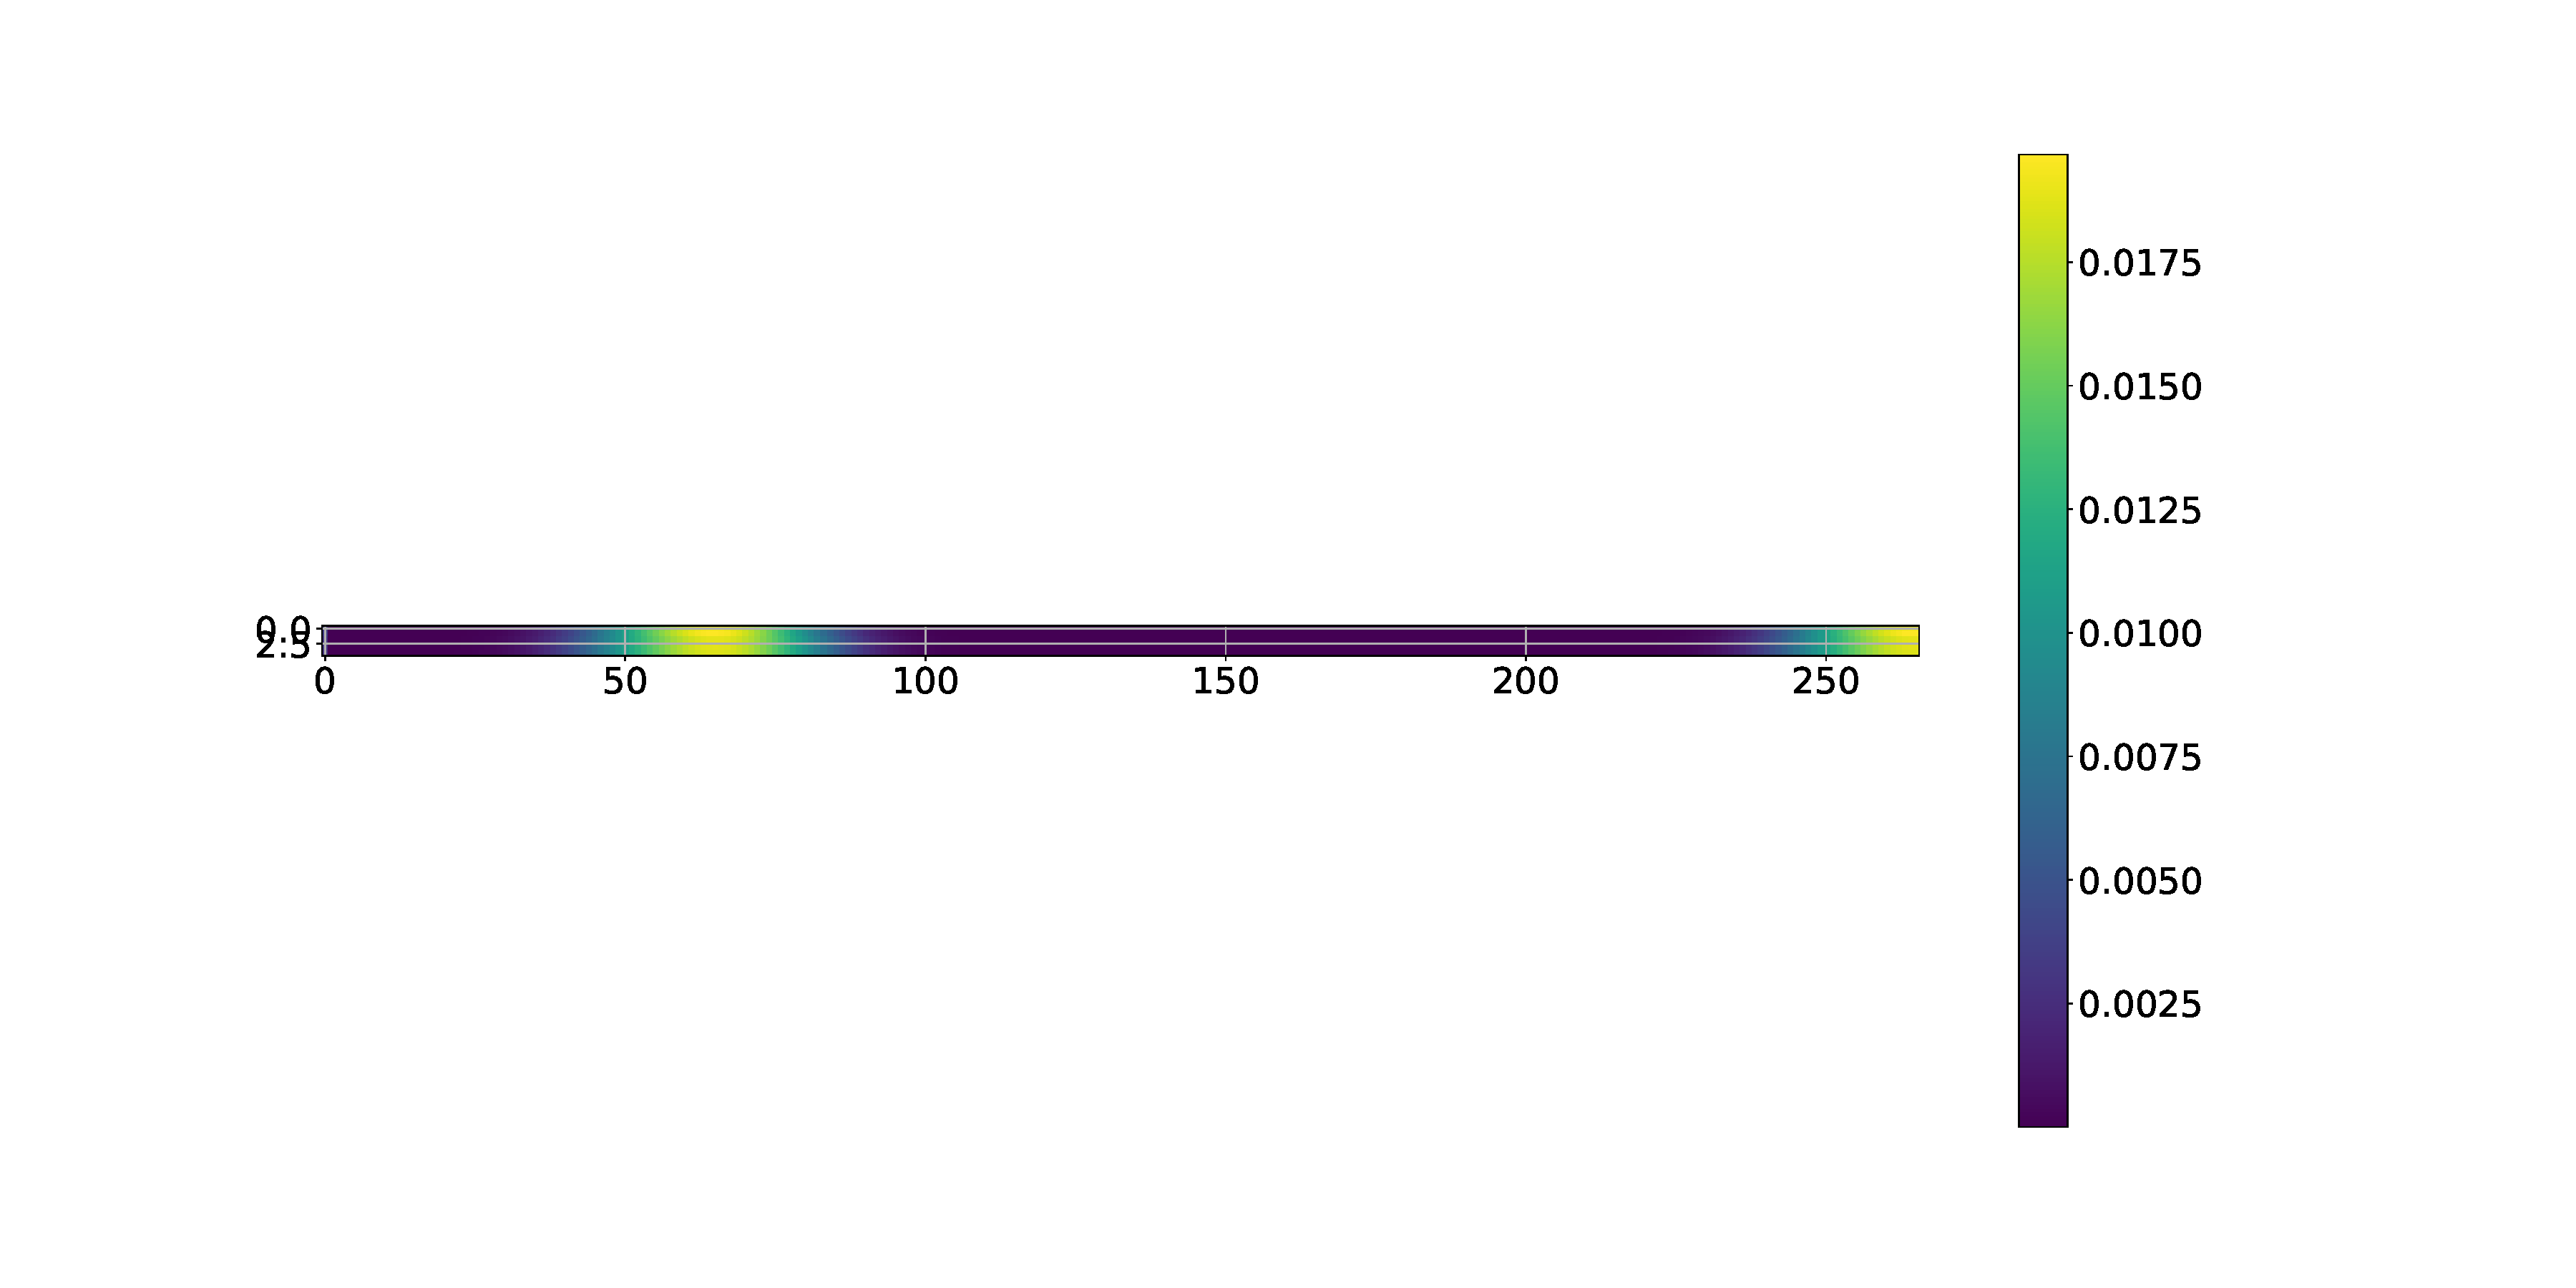
\includegraphics[width=0.5\textwidth]{figures/Attention1_2dim.pdf}}
\subfloat[]{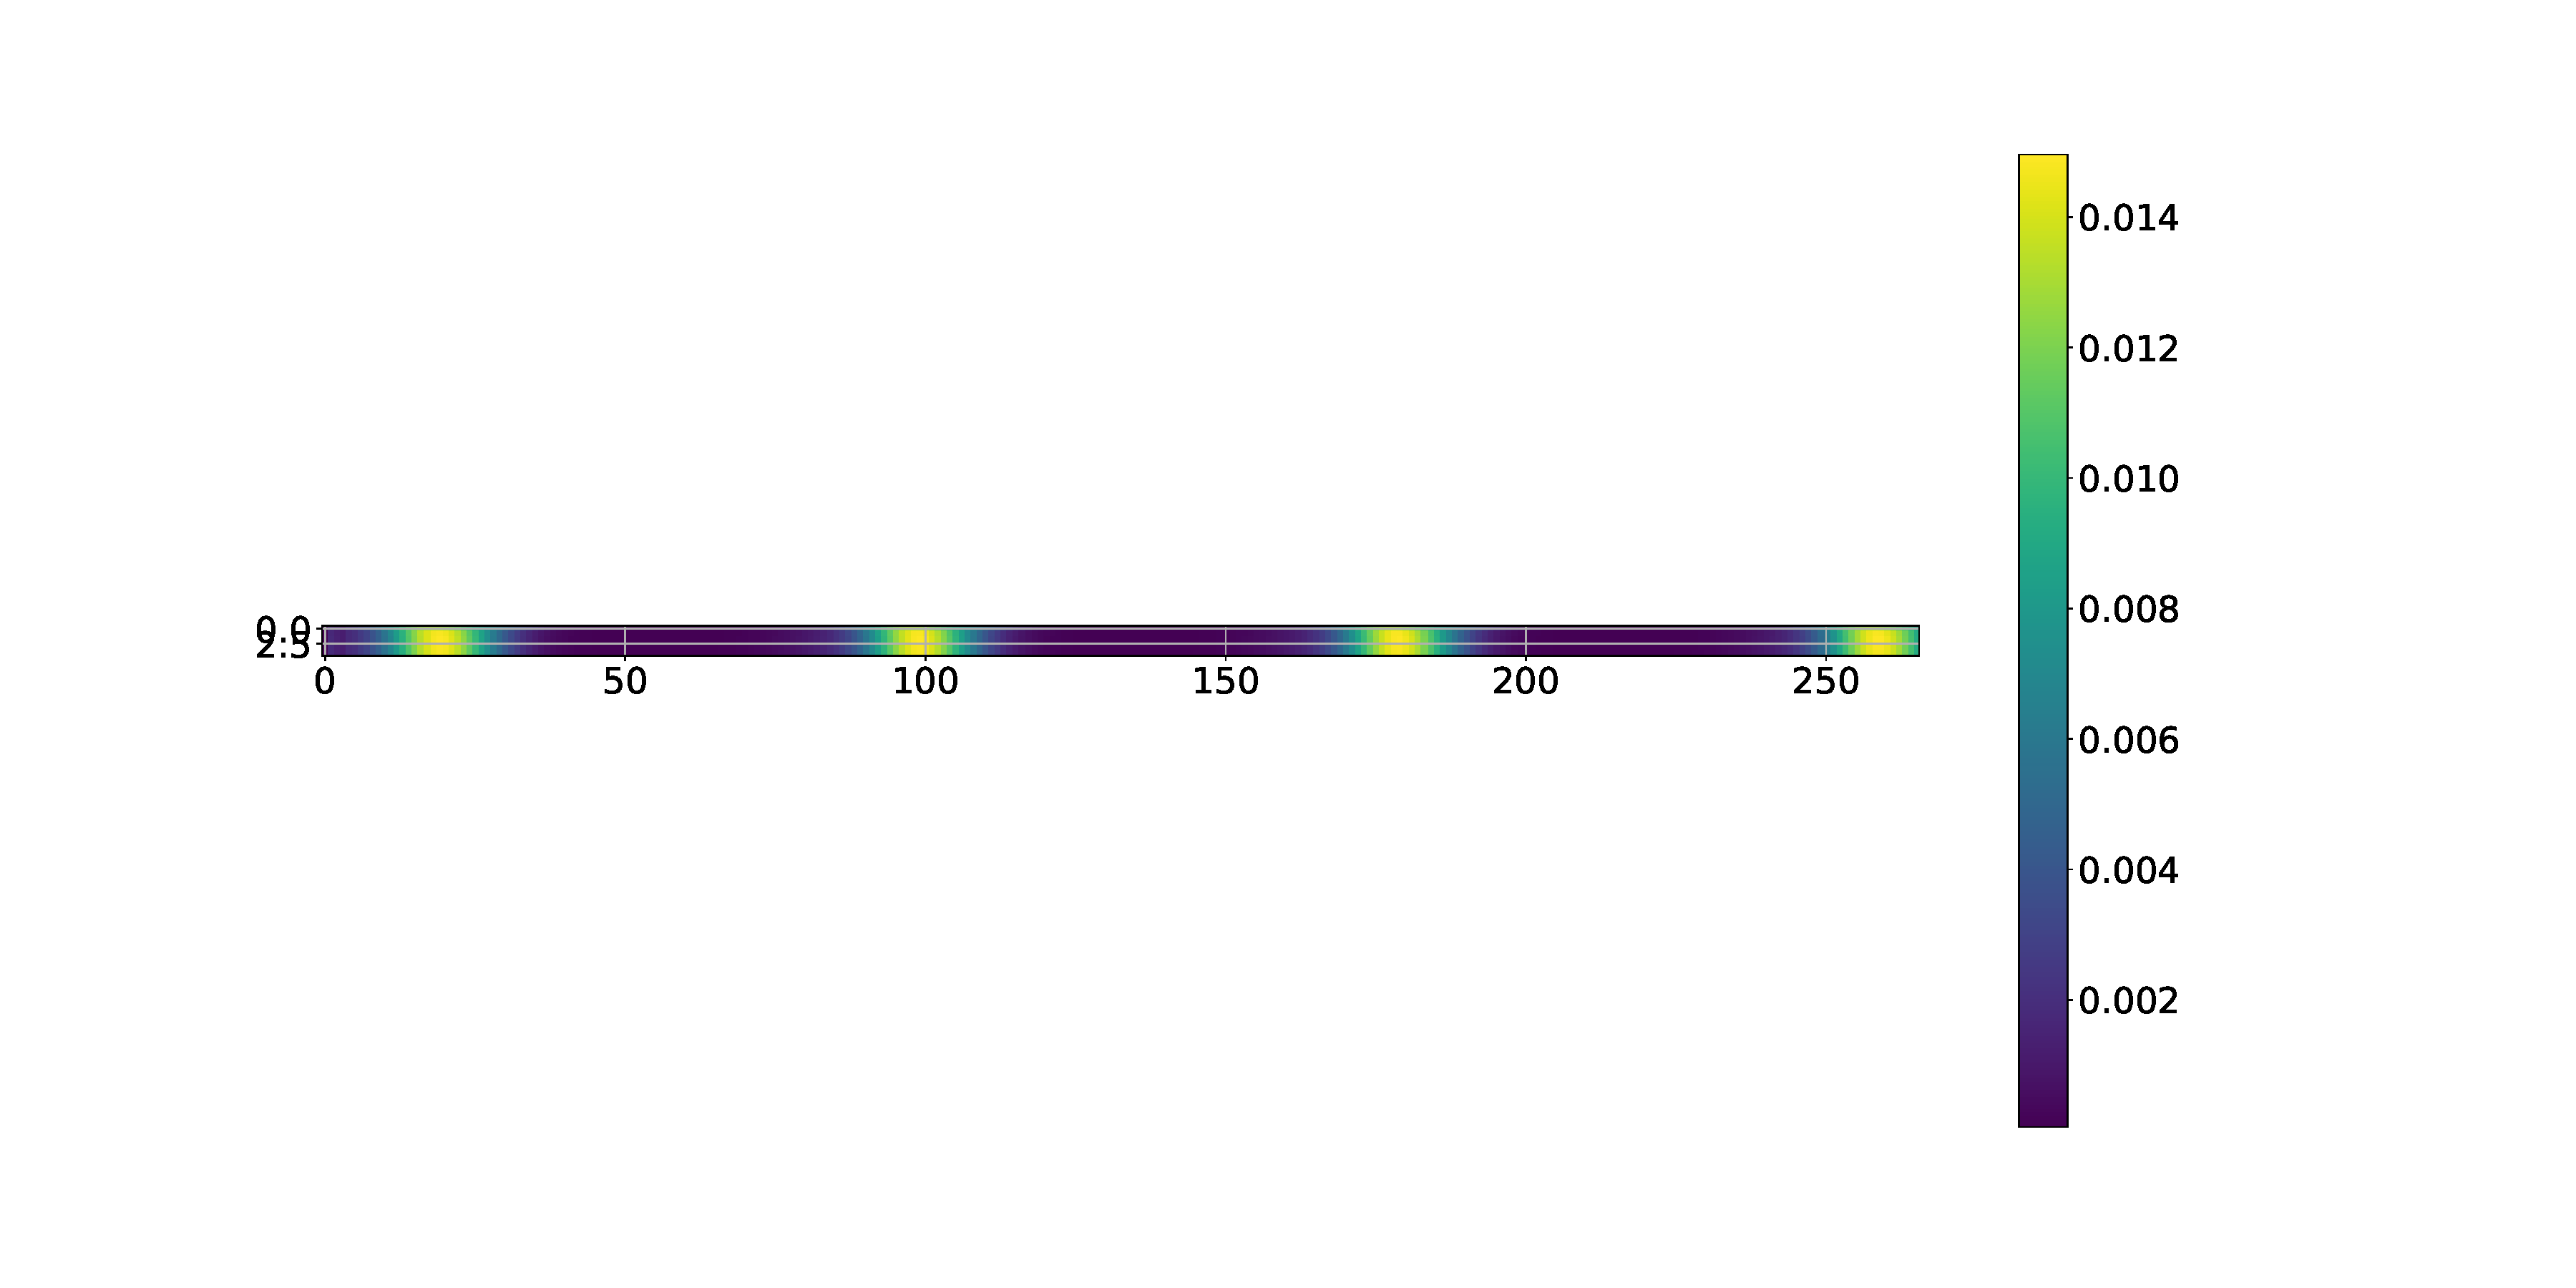
\includegraphics[width=0.5\textwidth]{figures/Attention2_2dim.pdf}}\\

\caption{Результаты для модели с рис.~\ref{fig1}}
\label{fig4}
\end{figure}

На рис.~\ref{fig4} показано, как для разных синусов выглядит скрытое пространство ecnoder'а, а также матрица Attention для генерации двух последующих точек в ряде.


\subsection{Эксперимент с простыми двумя простыми периодическими структурами внутри одного ряда}

Задача состоит в том, чтобы при помощи механизма Attention с временного ряда, который состоит из двух переодических сигналов (к примеру человек по очереди идет некоторое время и бежит некоторое время) выделить моменты времени где наблюдается первое действие и выделить моменты времени где наблюдается второе действие. 

Предлагается использовать seq2seq модель с Attention. 

Сама структура LSTM строит по сути фазовое пространство большой размерности. Попробуем обучить seq2seq модель, которая на вход принимает сигнал, который состоит из двух периодических сигналов, выдать на выход два сигнала, первый сигнал это чистый первый периодический сигнал со входа, а второй сигнал это второй периодический сигнал со входа. Тоесть другими словами, попробуем, сделать так, чтобы LSTM смогла из фазовому пространству вычленить два разных периодических сигнала. Для определенности будем считать первым периодическим сигналом тот сигнал который во временном ряде встретился раньше.

Как сделать чтобы LSTM по одному входу дала два сигнала???? У этого вопроса есть два возможных ответа:
\begin{itemize}
    \item первый случай простой, а давайте выход декодера будет не число а два числа --- значения первого сигнала и второго сигнала в один тик времени (простыми словами у нас есть 2 линейные модели которые по фазовому пространству делают некоторый предикт сигнала)
    
    \item второе решение немного сложнее (сейчас пробую сделать его). У нас есть как и раньше один выход LSTM. Но мы можем варьировать начальную точку LSTM с которой она начинает генерировать ряд. К примеру если мы хочем получить первый сигнал, что в качестве начальной точки дадим $0$ а если хочем сгенериить второй сигнал, то начальной точкой LSTM дадим $1$.
\end{itemize}
Ничего не получилось.

\begin{thebibliography}{99}
	\bibitem{cinar2018}
	\textit{Y. G. Cinar and H. Mirisaee} Period-aware content attention RNNs for time series forecasting with missing values~// Neurocomputing, 2018. Vol. 312. P. 177--186.
	
\end{thebibliography}

\end{comment}
\begin{comment}
\section{Предположения}

Введем следующие предположение:
\begin{itemize}
    \item Периоды всех сигналов прибьлизительно равны.\\
    Пока работаем с учетом данного предположения, потом можно будет попытаться избавиться от данного условия.
    \item Максимальный период $T$ сигналов известен.\\
    Пока работаем в случае, когда мы знаем количесво различных сигналов во временном ряде, после этого можно попытаться это улучшить.
    \item Известно количество $K$ различных сигналов.\\
    Пока работаем в случае, когда мы знаем количество различных сигналов во временном ряде, после этого можно будет попытаться это улучшить.
    \item Сигналы меняются не очень часто (подряд идет не менее 2-3 периодов одного сигнала)\\
    Это нужно чтобы фазовое пространство "успевало" установиться. Тоесть не было бы случая, когда у нас все время меняются временные ряды.
    \item Сигналы "достаточно" различны.\\
    Над этим надо подумать как это определить, но суть в том, что нельзя чтобы это был один и тот же синус с только разными амплитудами, тогда базисные вектора будет одинаковые. Это плохо только тогда, когда длину базисного вектора не учитываем(сингулярное число), а если учесть то на синусах тоже все работает. (Над этим пунктом нужно сильно подумать).
\end{itemize}
\end{comment}

\begin{center}
\bf
А.\,В.~Грабовой\footnote{Московский физико-технический институт, grabovoy.av@phystech.edu}, В.\,В.~Стрижов\footnote{Вычислительный центр им. А.~А. Дородницына	ФИЦ ИУ РАН, strijov@ccas.ru}

\end{center}

{\centering\begin{quote}
\textbf{Аннотация:} Данная работа посвящена поиску периодических сигналов во временных рядах с целью распознавания физических действий человека с помощью акселерометра. Предлагается метод кластеризации точек временного ряда для поиска характерных периодических сигналов внутри временного ряда. Для построения признакового описания используется метода главных компонент для локального снижения размерности фазового пространства. Для оценки близости двух периодических сигналов вычисляется расстояние между базисными векторами, которые получены методом главных компонент. Используя матрицу попарных расстояний между точками временного ряда выполняется кластеризация данных точек. Для анализа качества представленного алгоритма проводятся эксперименты на синтетических данных и данных полученных при помощи мобильного акселерометра.


\smallskip
\textbf{Ключевые слова}: временные ряды; кластеризация; распознание физической активности; метод главных компонент.

\smallskip
\textbf{DOI}: 00.00000/00000000000000
\end{quote}
}

\section{Введение}
Анализ повседневной физической активности человека производится при помощи мобильных телефонов, разумных часов. Портативные устройства используют акселерометр, гироскоп и магнитометр. Цель данной работы заключается в  распознавании и разметке человеческой активности во времени. %Некоторые сходства с данной задачей можно увидеть в работах по классификации временных рядов~\cite{Ignatov2015}, а также задача об обнаружении периодов активности~\cite{Olivares2012, cinar2018}.

Временные ряды это объекты сложной структуры, при классификации которых значимую роль играет построение признакового пространства. Для этой цели используются: экспертно заданные базовые функций, гипотеза порождения данных. В \cite{Ivkin2015} рассматривается комбинированное признаковое описание на основе данных методов. В \cite{Katrutsa2015} также рассматривается проблема построение признакового пространства и предлагается критерий избыточности выбранных признаков.

В данной работе рассмотрена задача \textit{кластеризации} точек временного ряда. Под \textit{кластеризацией} точек, подразумевается сопоставление каждой точке временного ряда некоторой метке, которая соответствует некоторому \textit{сегменту} временного ряда. \textit{Сегмент} временного ряда это часть временного ряда, которая соответсвует одному характерному физическому действию, например: один шаг при ходьбе, или один шаг при беге. Пример сегментов показан на  рис.~\ref{example_1}. На рис.~\ref{example_1} также показан пример кластеризации временного ряда, в котором ряд разбит на два характерных физических действия, полученных при помощи акселерометра.

Решение задачи кластеризации состоит из двух этапов. Во-первых предлагается алгоритм \textit{локальной} аппроксимации временного ряда при помощи метода главных компонент~\cite{Shiglavsi1997} для получения признакового описания временного ряда. Под \textit{локальной} аппроксимацией временного ряда подразумевается, что для признакового описания его точки используется не весь ряд, а только некоторая окрестность данной точки. Во-вторых рассматривается метрика в новом пространстве признакового описания. После получения расстояния между точками временного ряда используется метод кластеризации KMeans~\cite{Kanungo2000} для кластеризации точек временного ряда.

Для решения задачи кластеризации точек временного ряда вводится ряд предположений о данном ряде. Предполагается, что периоды всех различных сегментов различаются не значительно, причем известен максимальный период сегмента и количество различных сегментов внутри временного ряда. Также предполгается, что тип активности во времени меняется не часто, а также что фазовые траектории разных сегментов являются различными. 

Проверка и анализ метода проводится на синтетической и реальной выборках. Синтетическая выборка построенная при помощи суммы нескольких первых членов ряда Фурье со случайными коэффициентами. Реальные данные получены при помощи мобильного акселерометра, который снимал показания во время некоторой физической активности человека.



\section{Постановка}\label{statment}

\begin{figure}[h!t]\center
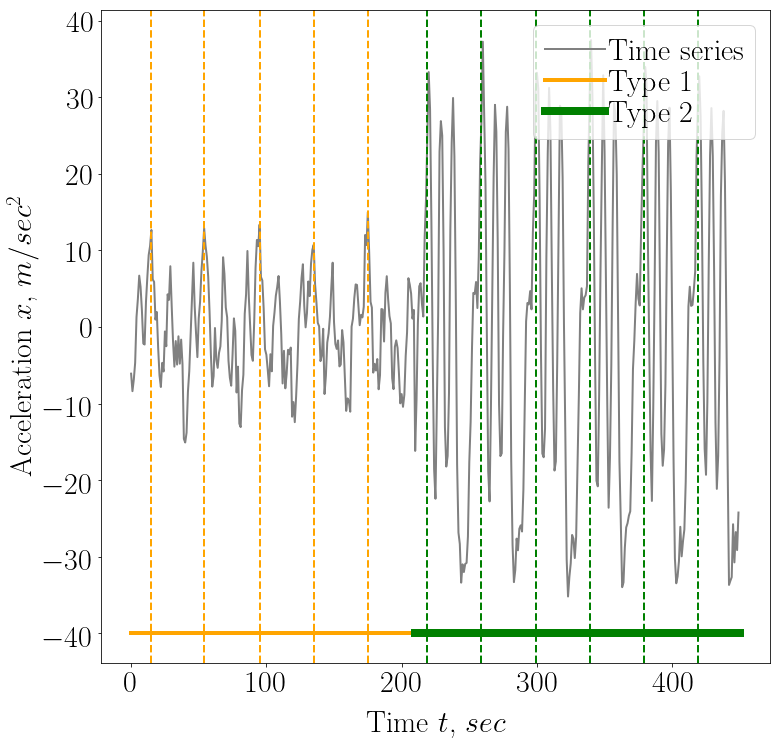
\includegraphics[width=1\textwidth]{results/example}\\
\caption{Временной ряд, с разметкой на кластеры.}
\label{example_1}
\end{figure}

Задан временной ряд:
$$\textbf{x} \in \mathbb{R}^{N}, \eqno(\ref{statment}.1)$$
где $N$ количество точек, которыми задается временной ряд.

Пусть временной ряд состоит из последовательности сигналов из множества $\mathbf{V}$:
$$\textbf{x} = [\textbf{v}_1, \textbf{v}_2, \cdots, \textbf{v}_M], \eqno(\ref{statment}.2)$$
где $\textbf{v}_i$ некоторый сигнал из множества возможных сигналов $\mathbf{V}$. Причем $\forall i$ выполняется или $\textbf{v}_i = \textbf{v}_{i-1}$ или   $\textbf{v}_i = \textbf{v}_{i+1}$. Пусть множество $\mathbf{V}$ удовлетворяет следующим свойствам:

$$\left|\mathbf{V}\right| = K, \quad \forall \textbf{v} \in \mathbf{V}~\left|\textbf{v}\right| \leq T, \eqno(\ref{statment}.3)$$
где $\left|\mathbf{V}\right|$ мощность множества сигналов, а $\left|\textbf{v}\right|$ длина сигнала.

Рассмотрим отображение:
$$a : x \to \{1,\cdots, K\}, \eqno(\ref{statment}.4)$$
где $x \in \textbf{x}$ некоторая точка временного ряда.

Требуется, чтобы отображение удовлетворяло следующим свойствам:

$$
\begin{cases}
    a\left(x_1\right) = a\left(x_2\right), & \text{если найдется}~\textbf{v} \in \mathbf{V}: x_1,x_2 \in \textbf{v}\\
    a\left(x_1\right) \not= a\left(x_2\right), & \text{если не найдется}~\textbf{v} \in \mathbf{V}: x_1,x_2 \in \textbf{v}
\end{cases}
$$

Пусть задана некоторая асессорская разметка временного ряда:
$$\textbf{y} \in \{1,\cdots,K\}^{N}. \eqno(\ref{statment}.5)$$

Тогда ошибка, которую совершает алгоритм $a$ на временном ряде $\textbf{x}$ представляется в следующем виде:
$$S = \frac{1}{N}\sum_{i=1}^{N}[y_i = a\left(x_i\right)], \eqno(\ref{statment}.6)$$
где $x_i$ --- точки временного ряда,  $y_i$ асессорская разметка временного ряда.

\section{Кластеризация точек}\label{solution}
Рассматривается фазовая траектория временного ряда $\textbf{x}$:
$$\mathbf{H} = \{\textbf{h}_t| \textbf{h}_t = [x_{t-T}, x_{t-T+1}, \cdots, x_{t}],~T\leq t\leq N\}. \eqno(\ref{solution}.1)$$

Фазовая траектория разбивается на фазовые подпространства из $2T$ векторов:
$$\mathbf{S} = \{\textbf{s}_t| \textbf{s}_t = [h_{t-2T}, h_{t-2T+1}, \cdots, h_{t}],~2T\leq t\leq N\}. \eqno(\ref{solution}.1)$$

{\bf Утверждение:}
Размерность $2T$ фазового подпространства является достаточным для построения локальной аппроксимирующей модели.

Каждое $T\text{-мерное }$ пространство $\textbf{s}_t$ проектируется на подпространство значительно меньшей размерности при помощи метода главных  компонент~$\textbf{z}_t~=~\textbf{W}_t\textbf{s}_t$. Получим представление базисных векторов $\textbf{W}_t$, а также собственные числа, которые соответствуют данным базисным векторам каждого подпространства $\textbf{s}_t$ в $T\text{-мерном}$ пространстве:
$$\mathbf{W} = \{\textbf{W}_t| \textbf{W}_t = [\textbf{w}^1_t, \textbf{w}^2_t]\}, \quad \bm{\Lambda} = \{\bm{\lambda}_t| \bm{\lambda}_t=[\lambda^1_t, \lambda^2_t]\}, \eqno(\ref{solution}.3)$$
где $[\textbf{w}^1_t, \textbf{w}^2_t]$ и $[\lambda^1_t, \lambda^2_t]$ это базисные векторы и соответствующие им собственные числа плоскости построенной при помощи метода главных компонент для подпространстве $\textbf{s}_t$.

Рассмотрим расстояние между элементами $\mathbf{W}$:

$$\rho\left(\textbf{W}_1, \textbf{W}_2\right) = \max_{\{\textbf{a},\textbf{b},\textbf{c}\} \subset \textbf{W}_1\cup \textbf{W}_2 } V\left(\textbf{a},\textbf{b},\textbf{c}\right), \eqno(\ref{solution}.4)$$
где $V\left(\textbf{a},\textbf{b},\textbf{c}\right)$ --- объем паралелепипеда построенного на векторах $\textbf{a}, \textbf{b}, \textbf{c}$.

{\bf Утверждение:}
$\rho\left(\textbf{W}_1, \textbf{W}_2\right)$ является метрикой, если дополнительно указать, что базисы соответсвующие параллельным плоскостям не различимы.\\

Рассмотрим расстояние между элементами $\bm{\Lambda}$:
$$\rho\left(\bm{\lambda}_1, \bm{\lambda}_2\right) = \sqrt[]{\left(\bm{\lambda}_1 - \bm{\lambda}_2\right)^{\mathsf{T}}\left(\bm{\lambda}_1 - \bm{\lambda}_2\right)}. \eqno(\ref{solution}.5)$$

$\rho\left(\bm{\lambda}_1, \bm{\lambda}_2\right)$ является метрикой в пространстве $\mathcal{L}$.

Матрица попарных расстояний между базисными векторами для временного ряда $\textbf{x}$:
$$\textbf{M}_{\text{c}} = [0, 1]^{N\times N}. \eqno(\ref{solution}.6)$$

Матрица попарных расстояний между собственными значениями для временного ряда $\textbf{x}$:
$$\textbf{M}_{\text{l}} = [0, 1]^{N\times N}. \eqno(\ref{solution}.7)$$

Используя выражения~(\ref{solution}.4-7) определим растояниие между двумя точками $t_1, t_2$ временного ряда:
$$\rho\left(t_1, t_2\right) = \rho\left(\textbf{W}_1, \textbf{W}_2\right) + \rho\left(\bm{\lambda}_1, \bm{\lambda}_2\right), \quad \textbf{M} = \textbf{M}_{\text{l}} + \textbf{M}_{\text{c}}, \eqno(\ref{solution}.8)$$
где $\rho\left(t_1, t_2\right)$ является метрикой, как сумма двух метрик. Матрица $\textbf{M}$ является матрицей попарных расстояний между двумя точками временного ряда.

Используя матрицу попарных расстояний $\textbf{M}$ выполним кластеризацию моментов времени временного ряда, получим следующее отображение:

$$a : x \to \{1,\cdots, K\}, \eqno(\ref{solution}.9)$$
где $x$ некоторая точка временного ряда \textbf{x}.


\section{Эксперимент}\label{experiment}
Для анализа свойств предложенного алгоритма был проведен вычислительный эксперимент в котором кластеризация точек временного ряда проводилась используя матрицы попарных расстояний ~$(\ref{solution}.6-8)$.

В качестве данных использовались две выборки временных рядов, которые описаны в таблице~\ref{table_1}. Выборка Physical Motion это реальные временные ряды полученные при помощи мобильного акселерометра. Синтетические временные ряды были построены при помощи нескольких первых слагаемых ряда Фурье со случайными коэффициентами из стандартного нормального распределения. Генерация данных состояла из двух этапов. На первом этапе генерировались короткие сигналы $\textbf{v}$ для построения множества $\mathbf{V}$. Вторым этапом генерации выборки $\textbf{x}$ является следующим случайным процессом:
$$\textbf{x} = [\textbf{v}_{1}, \textbf{v}_{2}, \cdots, \textbf{v}_{M}], \quad \begin{cases}
    \textbf{v}_{1} \sim \mathcal{U}\left(\mathbf{V}\right),\\
    \textbf{v}_{i} = \textbf{v}_{i - 1}, & \text{с вероятностью}~\frac{3}{4}\\
    \textbf{v}_{i} \sim \mathcal{U}\left(\mathbf{V}\right), & \text{с вероятностью}~\frac{1}{4}
\end{cases}, \eqno(\ref{experiment}.1)$$
где $\mathcal{U}\left(\mathbf{V}\right)$ --- равномерное распределение на объектах из $\mathbf{V}$.

\begin{table}[h]
\begin{center}
\caption{Описание выборок}
\label{table_1}
\begin{tabular}{|c|c|c|c|}
\hline
	Ряд & $N$& $K$& $T$\\
	\hline
	\multicolumn{1}{|l|}{Physical Motion 1}
	& 900& 2& 30\\
	\hline
	\multicolumn{1}{|l|}{Physical Motion 2}
	& 1000& 2& 30\\
	\hline
	\multicolumn{1}{|l|}{Synthetic 1}
	& 2000& 2& 20\\
	\hline
	\multicolumn{1}{|l|}{Synthetic 2}
	& 2000& 3& 20\\
\hline

\end{tabular}
\end{center}
\end{table}

\paragraph{Синтетические данные.}

\begin{figure}[h!t]\center
\subfloat[Synthetic 1]
{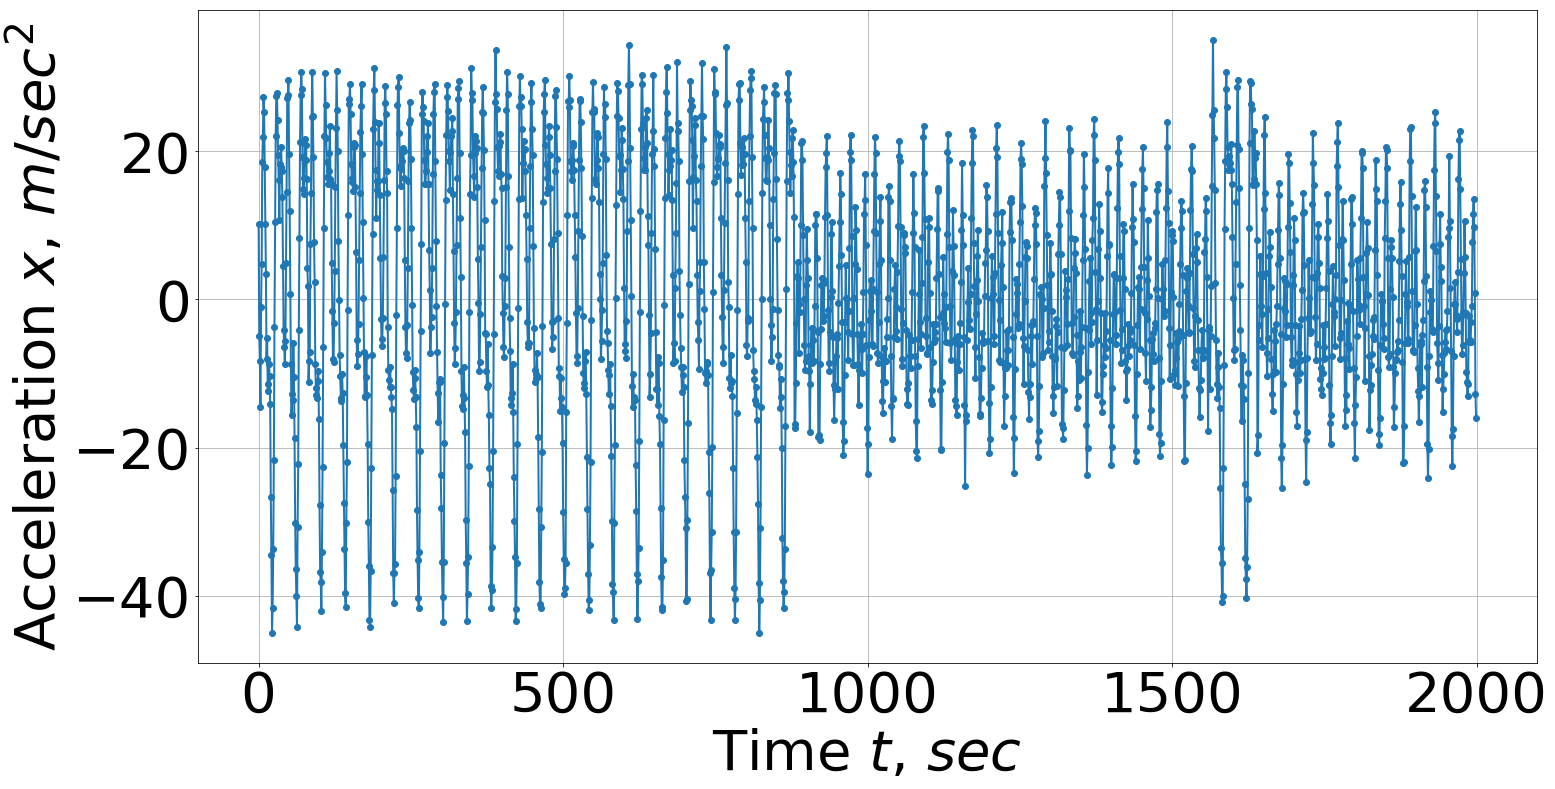
\includegraphics[width=0.5\textwidth]{results/2_patern_series}\label{fig_synthetic_series_2}}
\subfloat[Synthetic 2]
{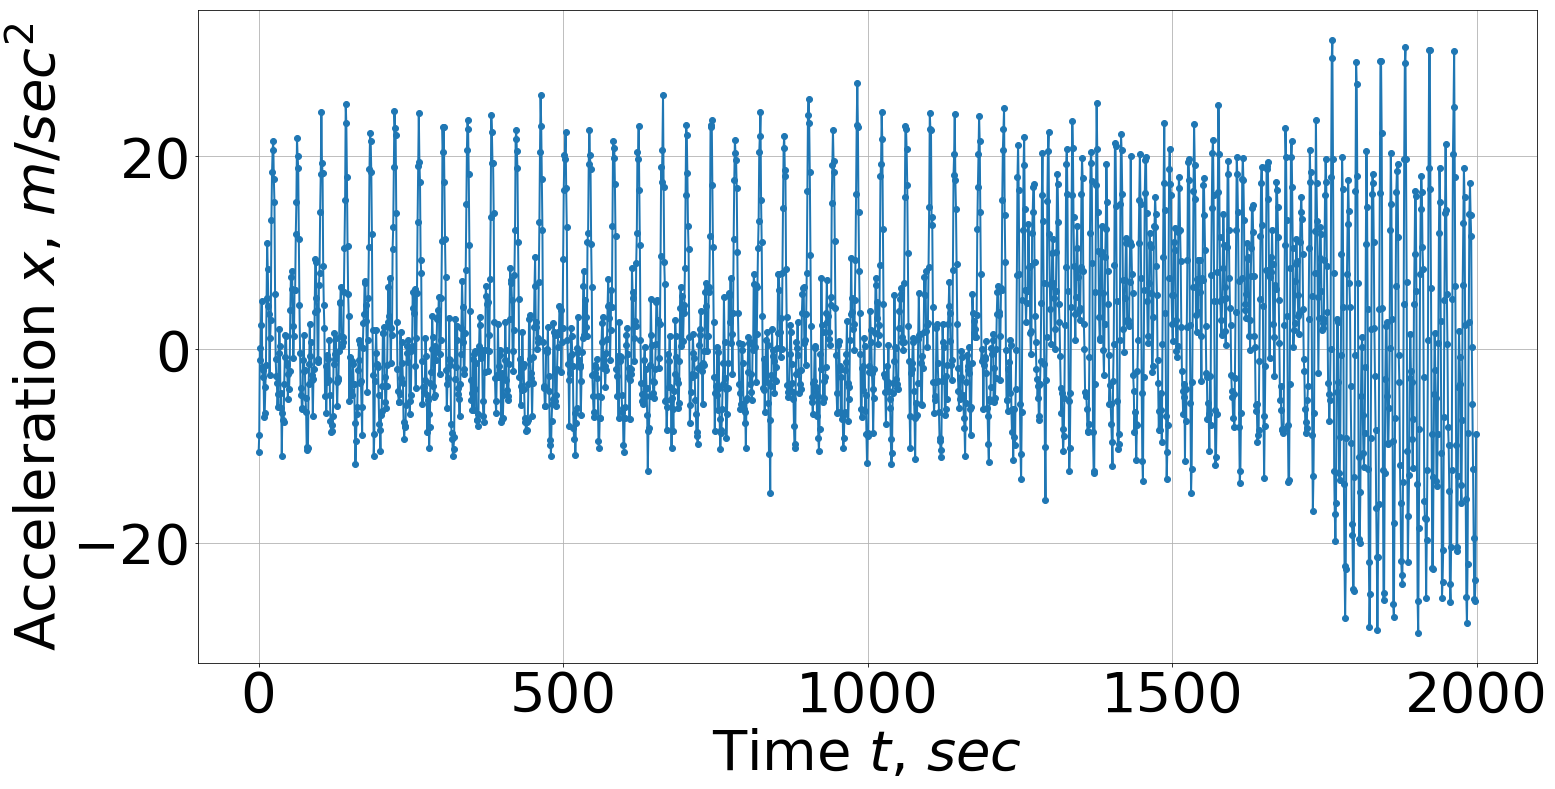
\includegraphics[width=0.5\textwidth]{results/3_patern_series}\label{fig_synthetic_series_3}}\\
\caption{Пример синтетически построенных временных рядов}
\label{fig_synthetic_series}
\end{figure}

На рис.~\ref{fig_synthetic_series} приведен пример синтетически построенных временных рядов. На рис.~\ref{fig_synthetic_series_2} показан пример ряда в котором количество сигналов $K = 2$, а длина каждого сигнала $T = 20$. На рис.~\ref{fig_synthetic_series_3} показан пример ряда в котором количество сигналов $K = 3$, а длина каждого сигнала $T = 20$. 

\begin{figure}[h!t]\center
\subfloat[Synthetic 1]
{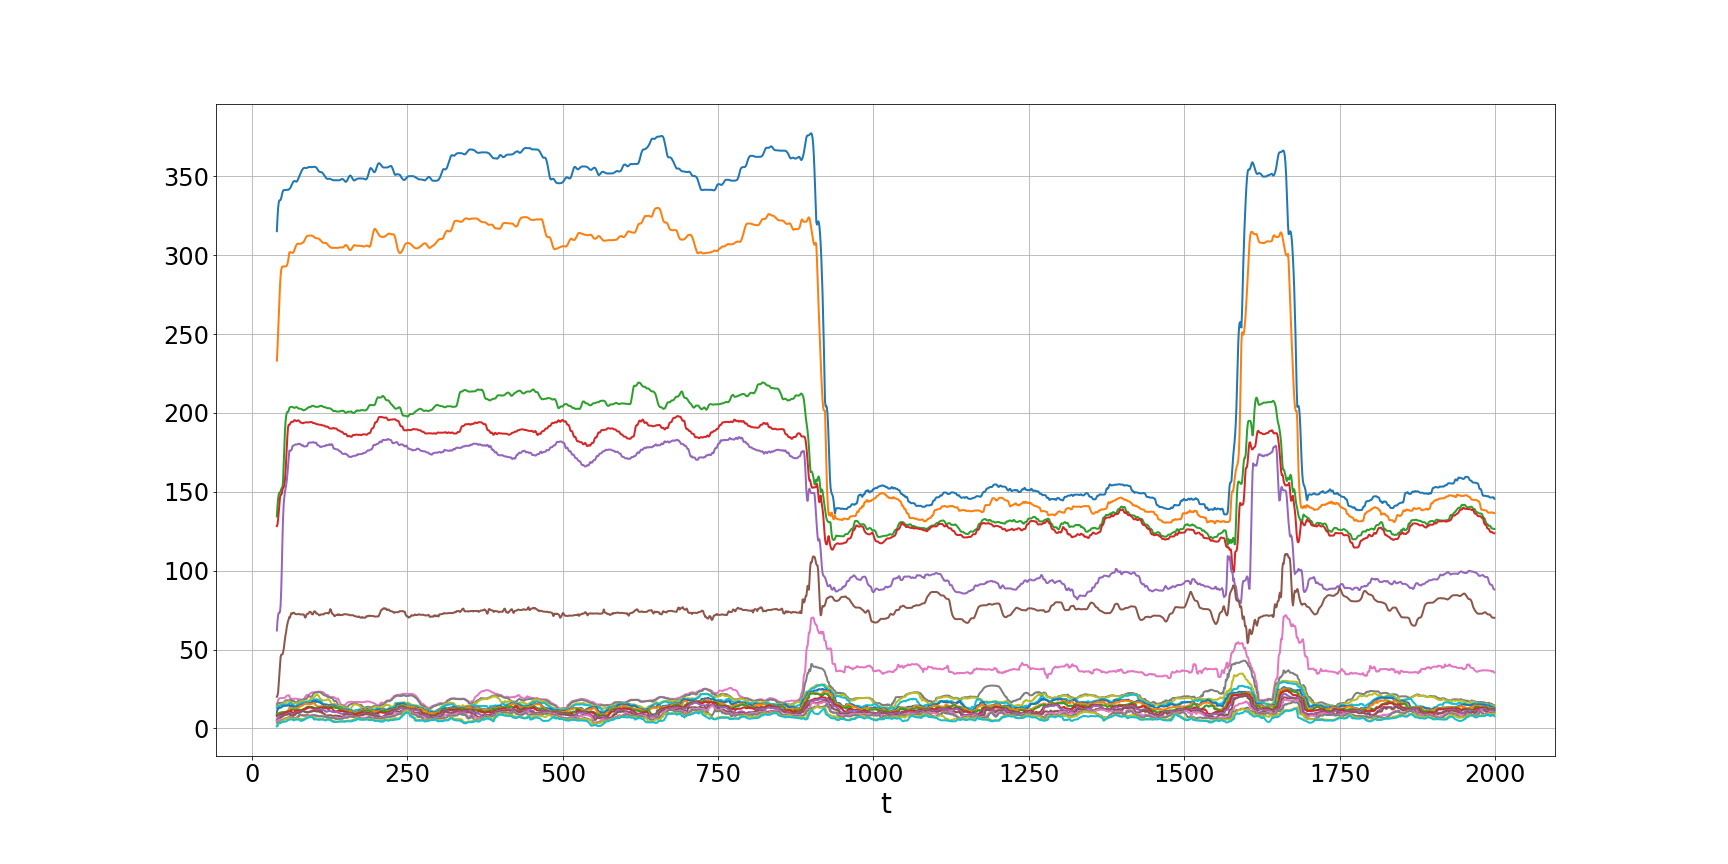
\includegraphics[width=0.5\textwidth]{results/2_patern_lambda}}
\subfloat[Synthetic 2]
{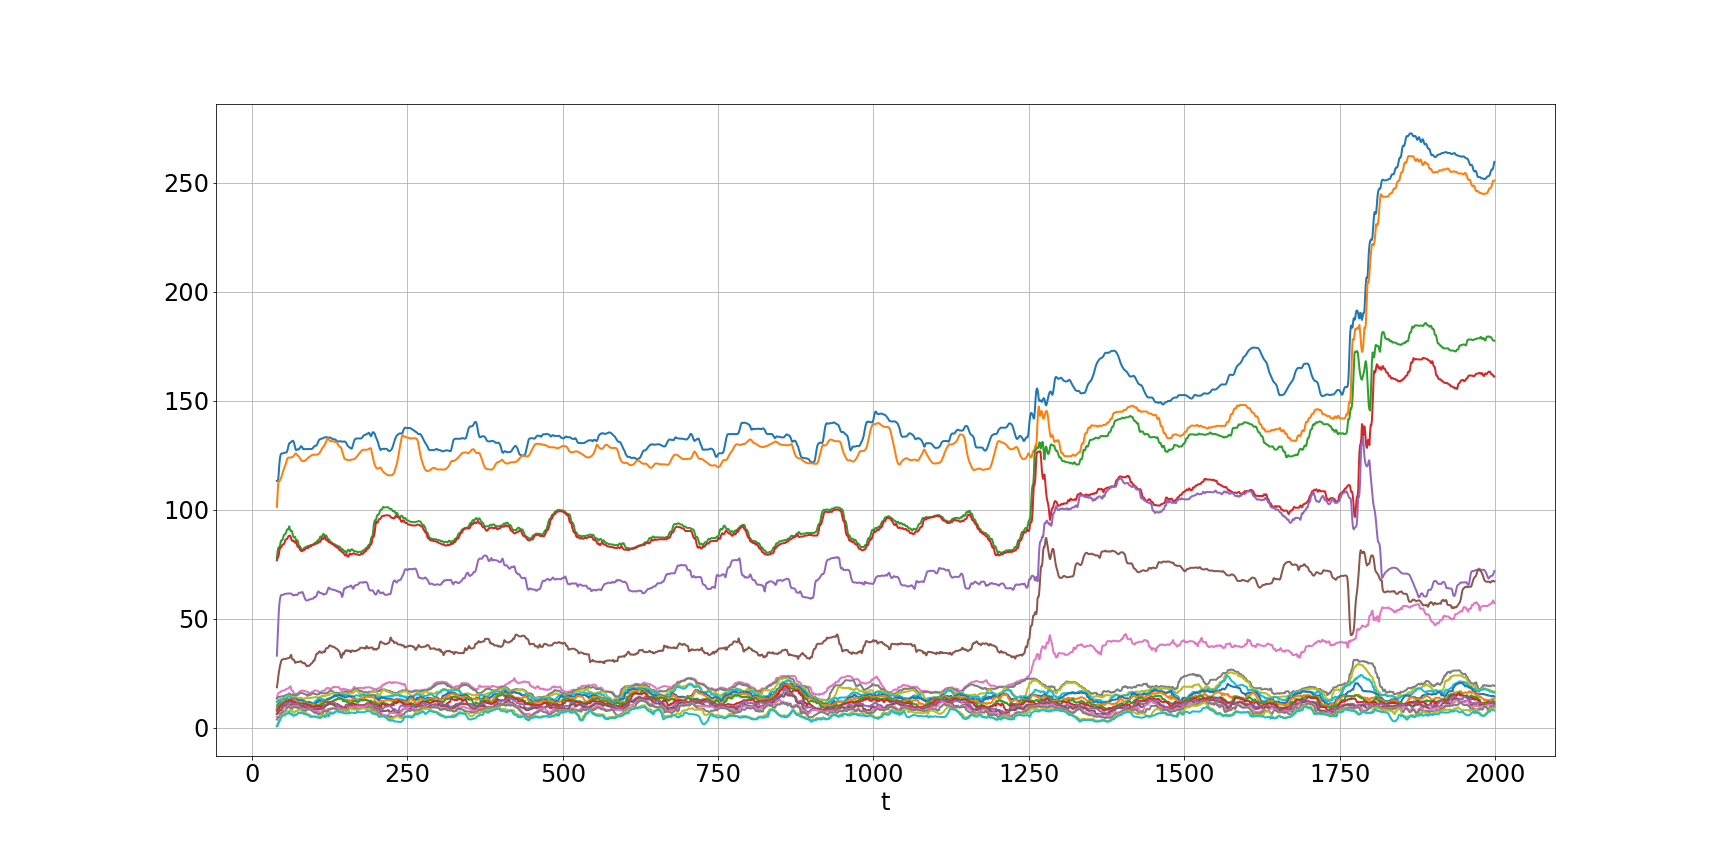
\includegraphics[width=0.5\textwidth]{results/3_patern_lambda}}\\
\caption{График зависимости значения сингулярных чисел метода главных компонент}
\label{fig_synthetic_lambda}
\end{figure}

\begin{figure}[h!t]\center
\subfloat[Synthetic 1]
{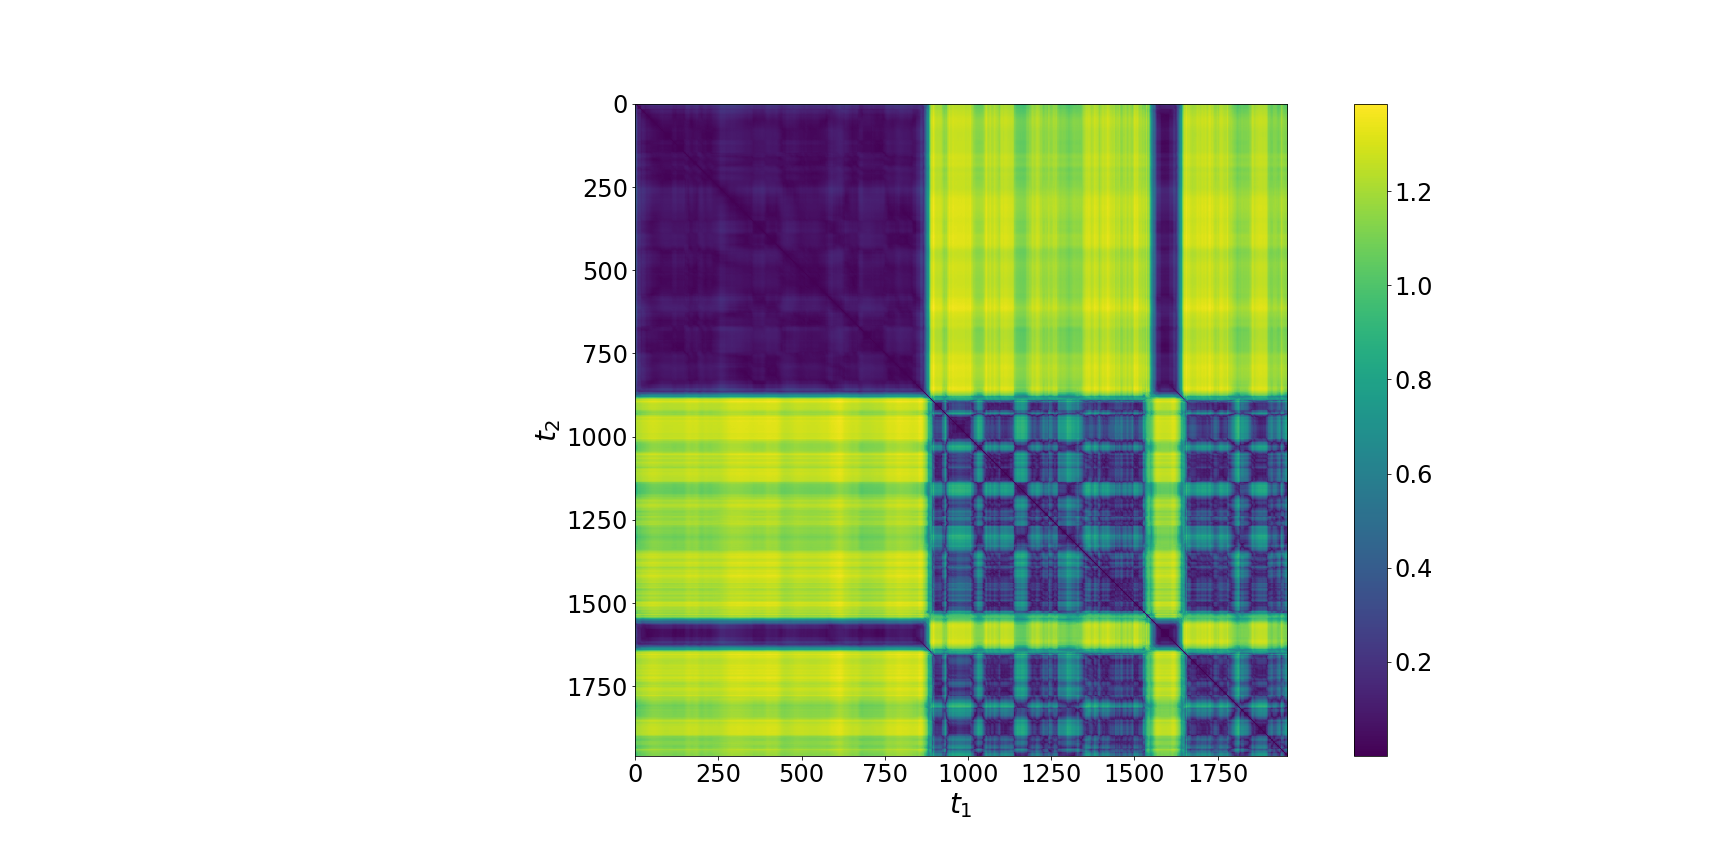
\includegraphics[width=0.5\textwidth]{results/2_patern_full}}
\subfloat[Synthetic 2]
{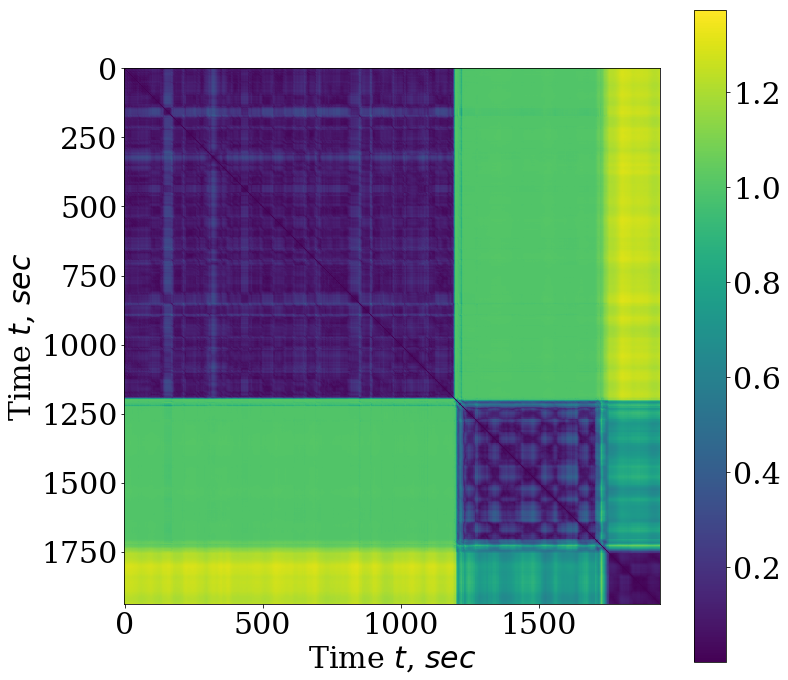
\includegraphics[width=0.5\textwidth]{results/3_patern_full}}\\
\caption{Матрица попарных расстояний $\textbf{M}$ между точками временного ряда}
\label{fig_synthetic_distance}
\end{figure}

На рис.~\ref{fig_synthetic_lambda} показан график зависимости значения сингулярных чисел локальной аппроксимации с течением времени. Значение сингулярных чисел, которые соответствуют первым двум главным компонентам значительно меняются с течением времени $t$. 

\begin{figure}[h!t]\center
\subfloat[Synthetic 1]
{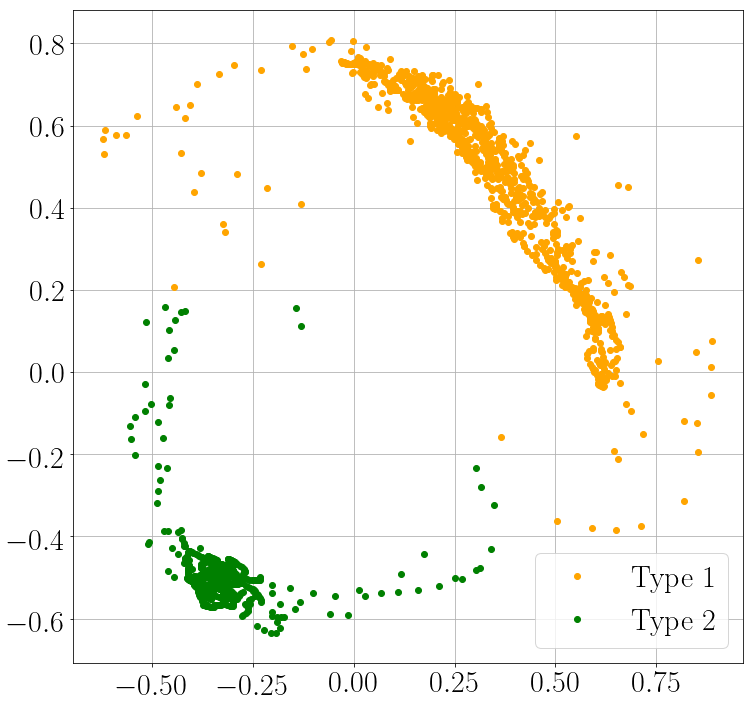
\includegraphics[width=0.5\textwidth]{results/2_patern_2D_vector}}
\subfloat[Synthetic 2]
{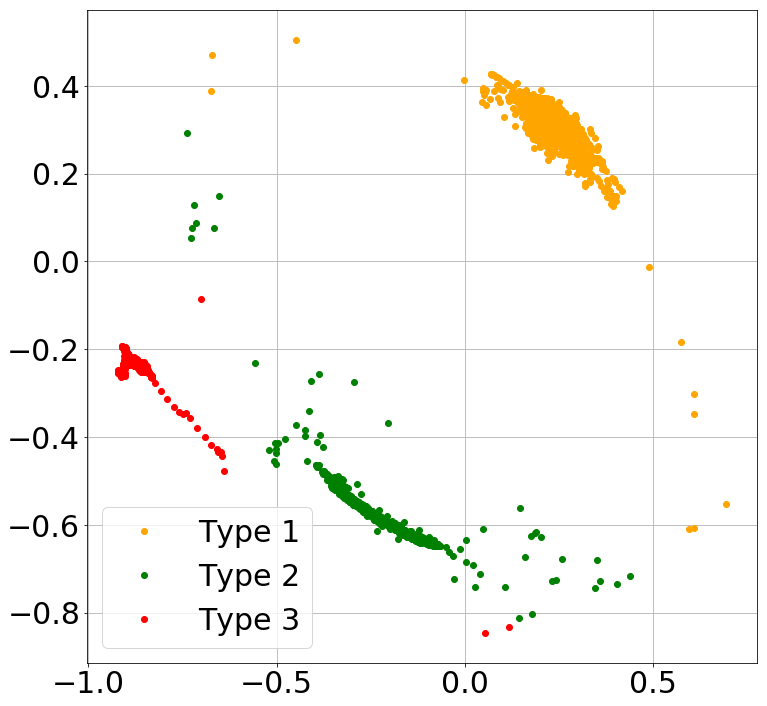
\includegraphics[width=0.5\textwidth]{results/3_patern_2D_vector}}\\
\caption{Проекция точек временного ряда на плоскость при помощи матрицы попарных расстояний $\textbf{M}$}
\label{fig_synthetic_2D}
\end{figure}


\begin{figure}[h!t]\center
\subfloat[Synthetic 1]
{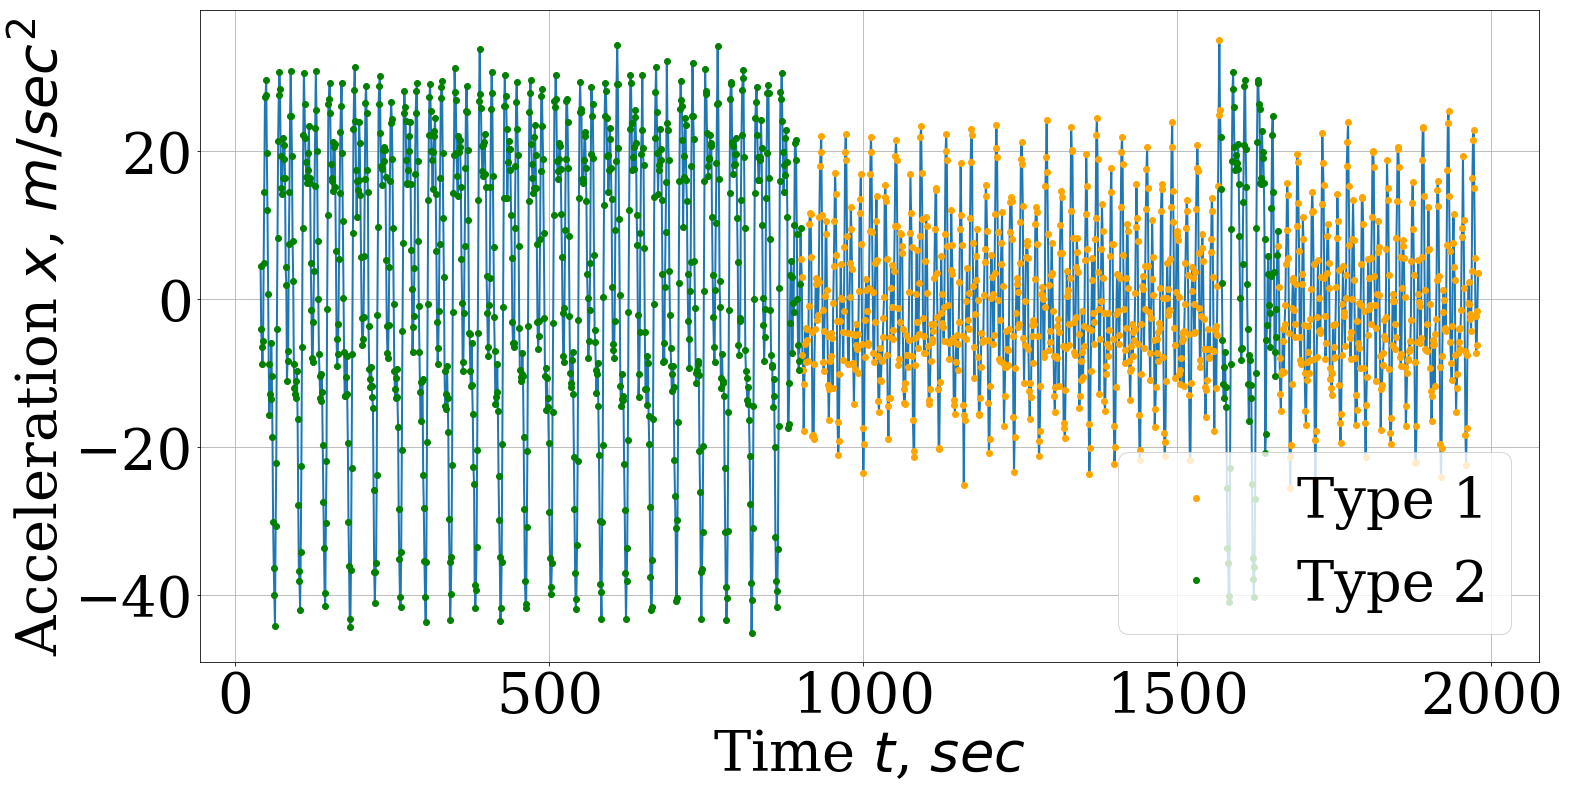
\includegraphics[width=0.5\textwidth]{results/2_patern_claster_vector}}
\subfloat[Synthetic 2]
{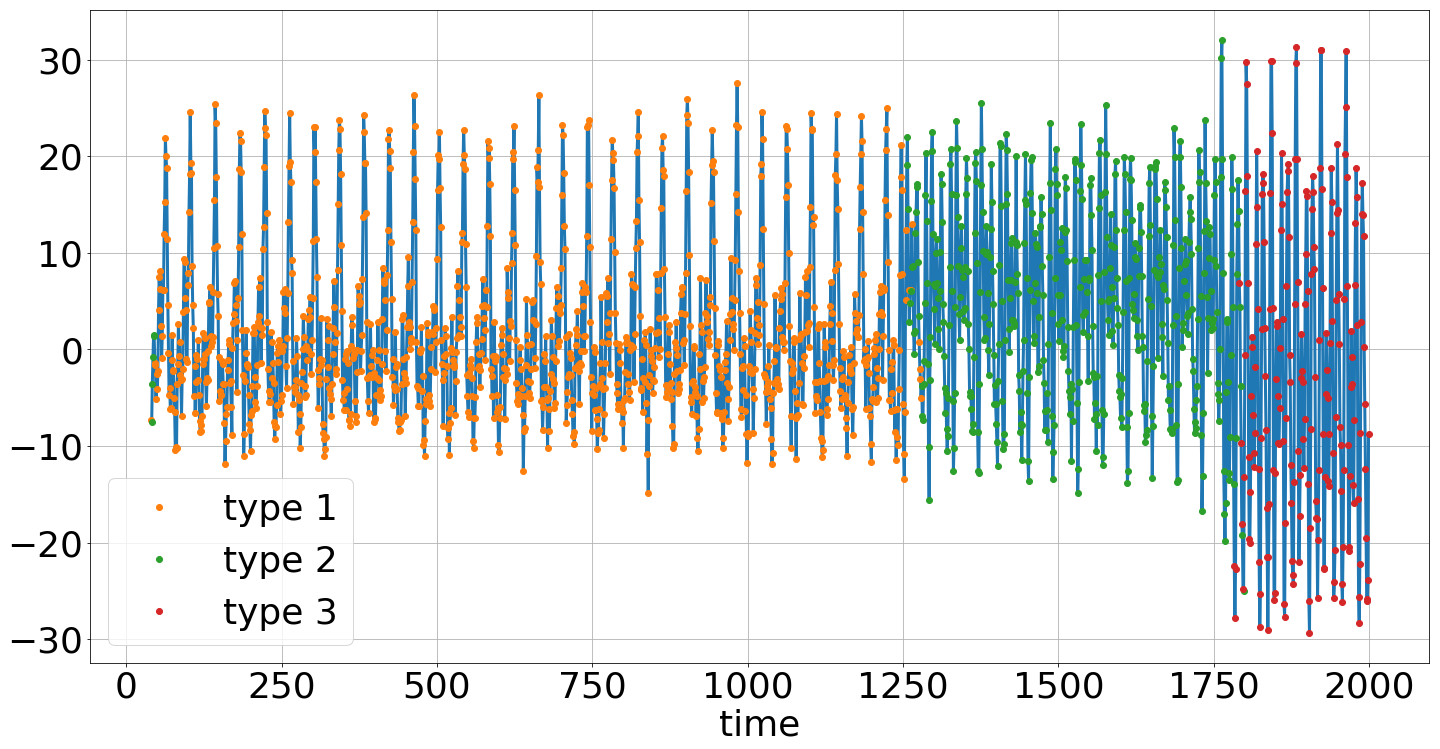
\includegraphics[width=0.5\textwidth]{results/3_patern_claster_vector}}\\
\caption{Кластеризация точек временного ряда}
\label{fig_synthetic_claster}
\end{figure}

На рис.~\ref{fig_synthetic_distance} проиллюстрированы матрицы попарных расстояний $\textbf{M}$ между построены при помощи формулы~$(\ref{solution}.8)$. Используя матрицу попарных расстояний и метод Multidimensional Scaling~\cite{Borg2005} визуальзуализируем точки временного ряда на плоскости. На рис.~\ref{fig_synthetic_2D} показана визуализация точек на плоскости и выполнена их кластеризация при помощи метода KMeans~\cite{Kanungo2000}. Иллюстрация кластеров точек временного ряда продемонстрирована на рис.~\ref{fig_synthetic_claster}.

\paragraph{Реальные данные.}
\begin{figure}[h!t]\center
\subfloat[Physical Motion 1]
{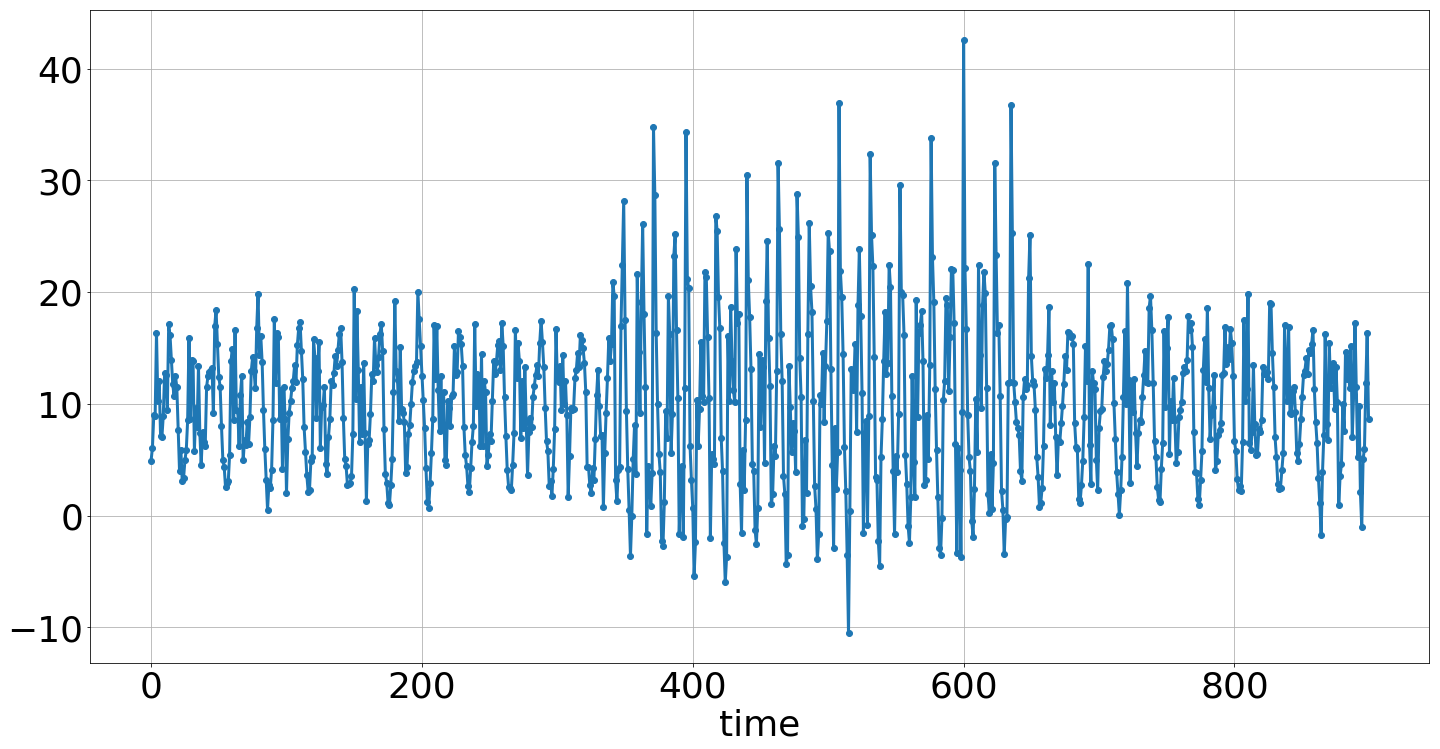
\includegraphics[width=0.5\textwidth]{results/1_real_series}}
\subfloat[Physical Motion 2]
{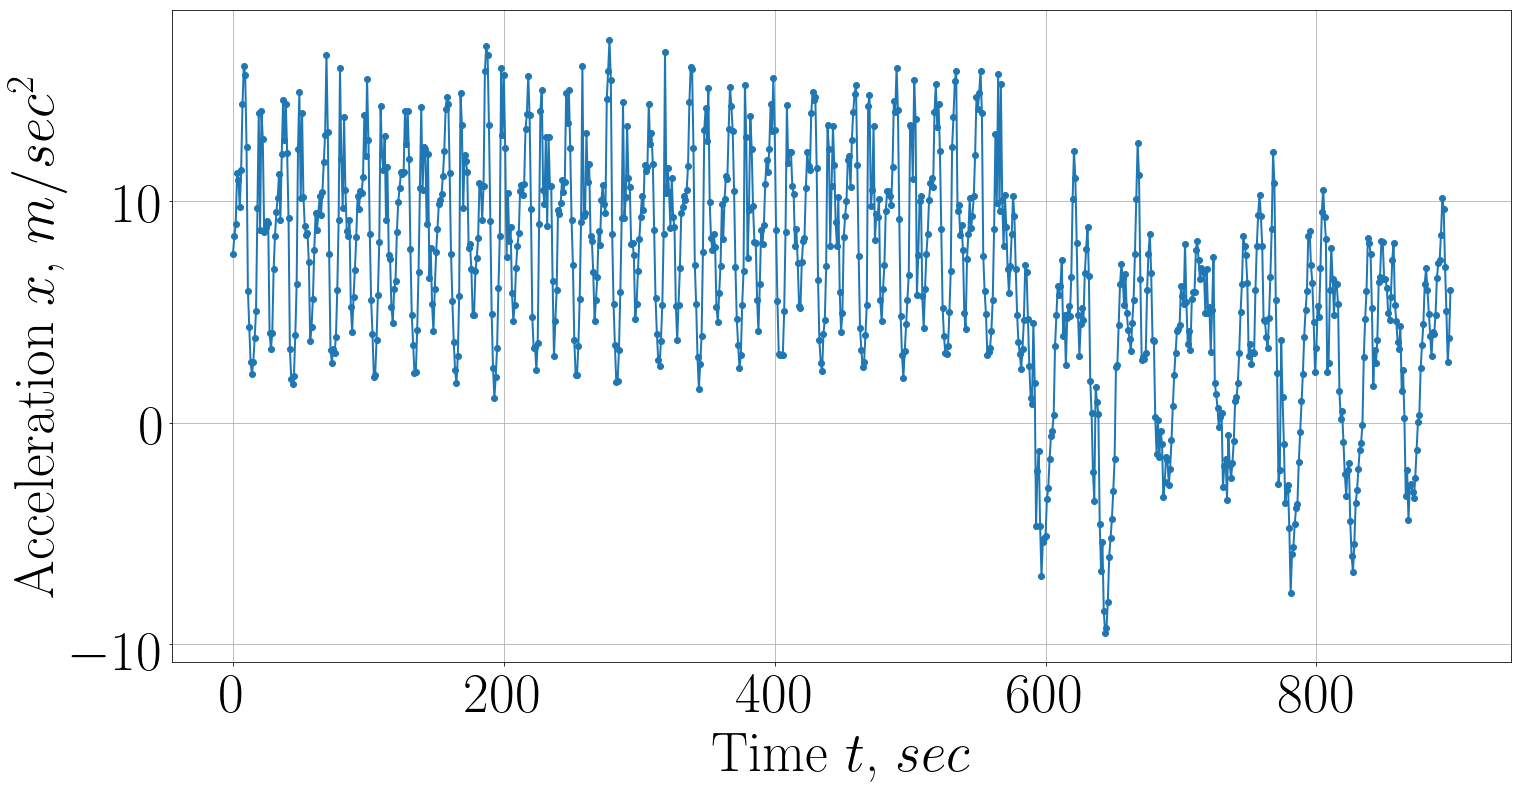
\includegraphics[width=0.5\textwidth]{results/2_real_series}}\\
\caption{Пример синтетически построенных временных рядов}
\label{fig_real_series}
\end{figure}

На рис.~\ref{fig_real_series} приведен пример реальных временных рядов полученных при помощи взятия одной из координат мобильного акселерометра. 

\begin{figure}[h!t]\center
\subfloat[Physical Motion 1]
{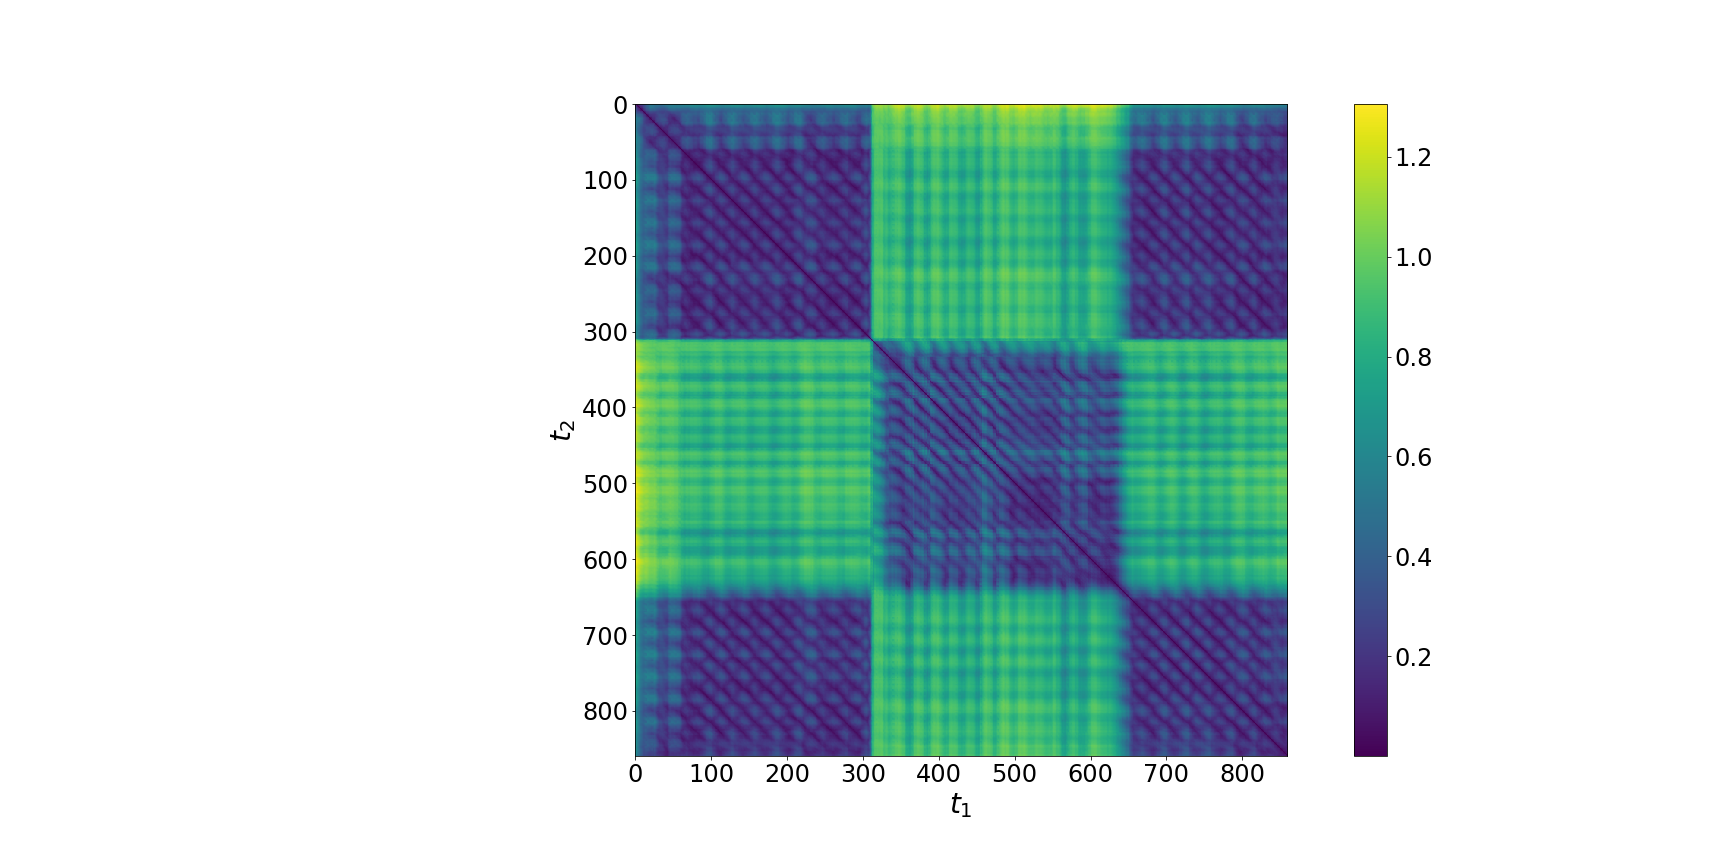
\includegraphics[width=0.5\textwidth]{results/1_real_full}}
\subfloat[Physical Motion 2]
{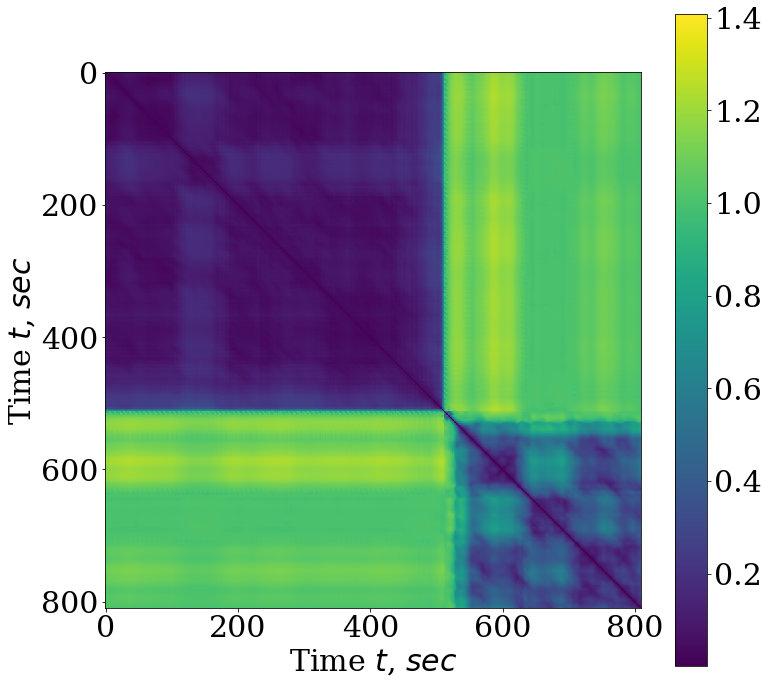
\includegraphics[width=0.5\textwidth]{results/2_real_full}}\\
\caption{Матрица попарных расстояний $\textbf{M}$ между точками временного ряда}
\label{fig_real_distance}
\end{figure}

На рис.~\ref{fig_real_distance} проиллюстрированы матрицы попарных расстояний $\textbf{M}$ между построены при помощи формулы~$(\ref{solution}.8)$. Используя матрицу попарных расстояний и метод Multidimensional Scaling~\cite{Borg2005} визуальзуализируем точки временного ряда на плоскости. На рис.~\ref{fig_real_2D} показана визуализация точек на плоскости и выполнена их кластеризация при помощи метода KMeans~\cite{Kanungo2000}. Иллюстрация кластеров точек временного ряда продемонстрирована на рис.~\ref{fig_real_claster}.


\begin{figure}[h!t]\center
\subfloat[Physical Motion 1]
{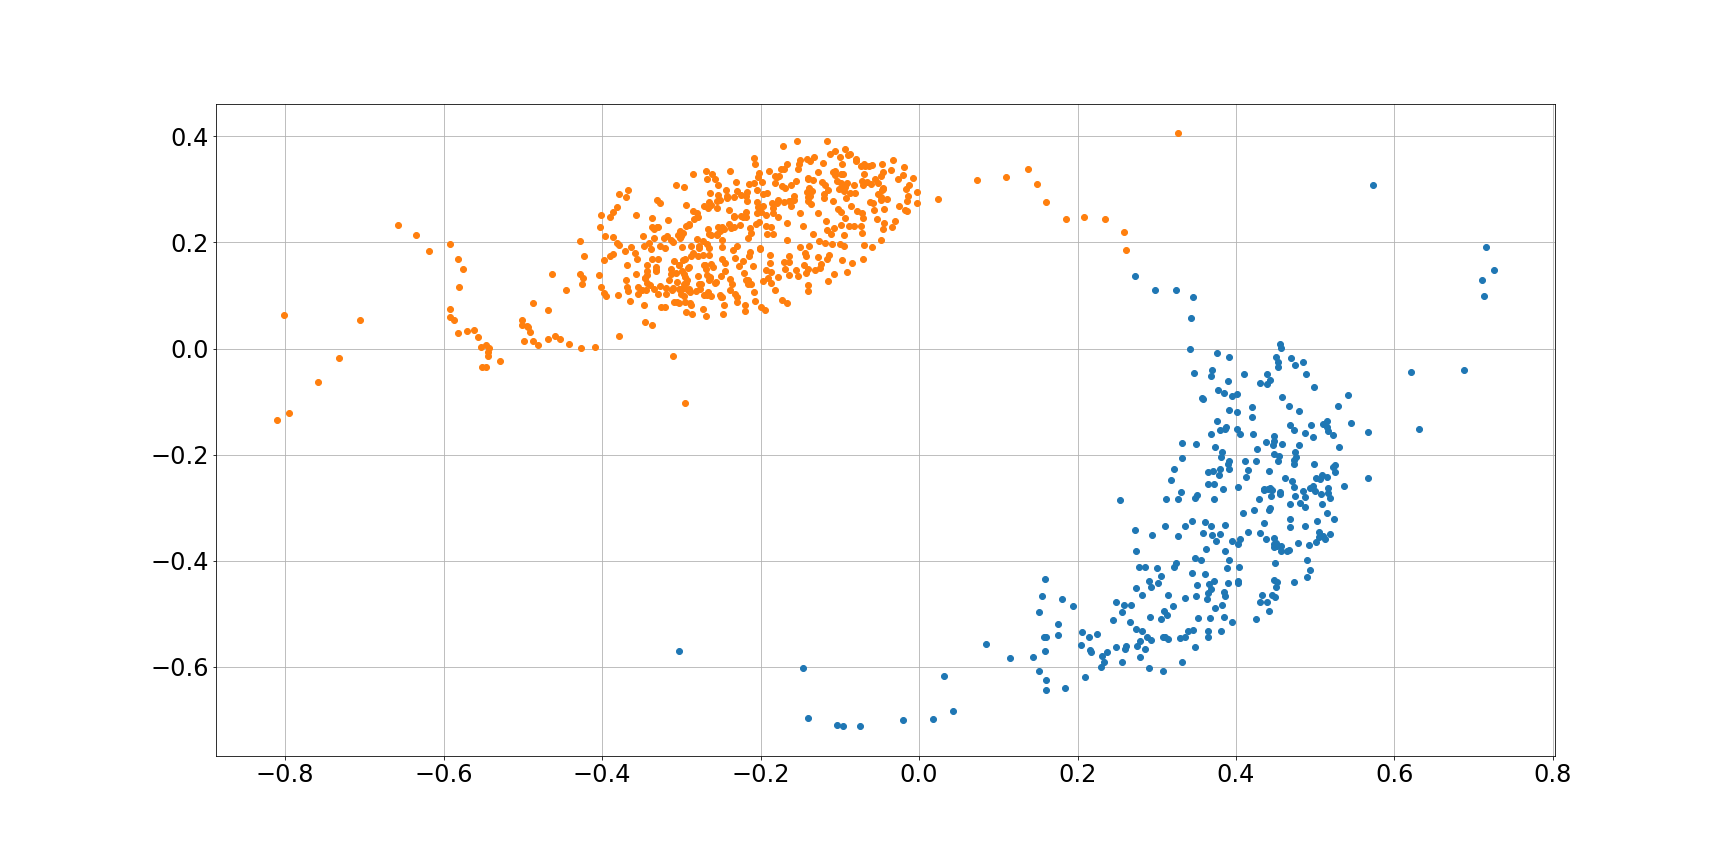
\includegraphics[width=0.5\textwidth]{results/1_real_2D_vector}}
\subfloat[Physical Motion 2]
{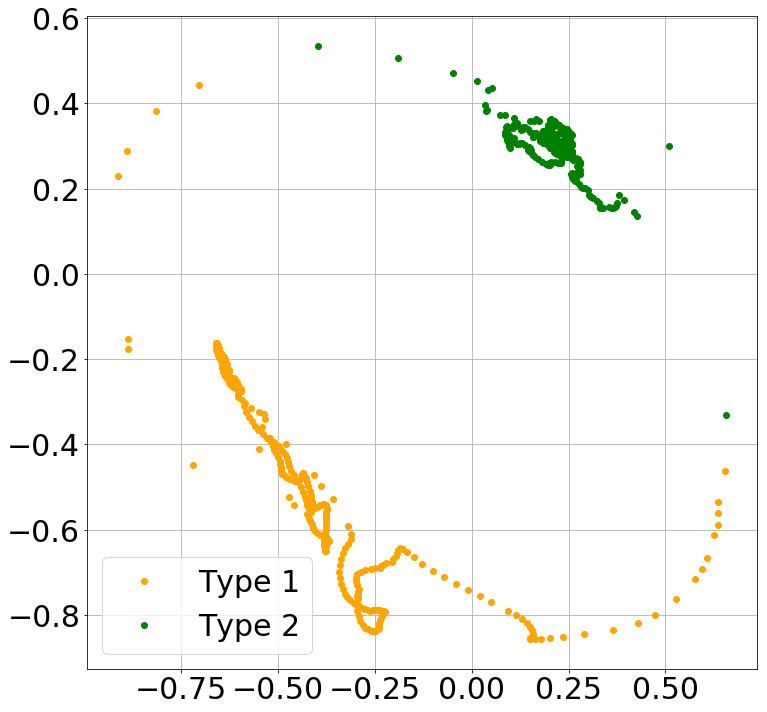
\includegraphics[width=0.5\textwidth]{results/2_real_2D_vector}}\\
\caption{Проекция точек временного на плоскость при помощи матрицы попарных расстояний $\textbf{M}$}
\label{fig_real_2D}
\end{figure}

\begin{figure}[h!t]\center
\subfloat[Physical Motion 1]
{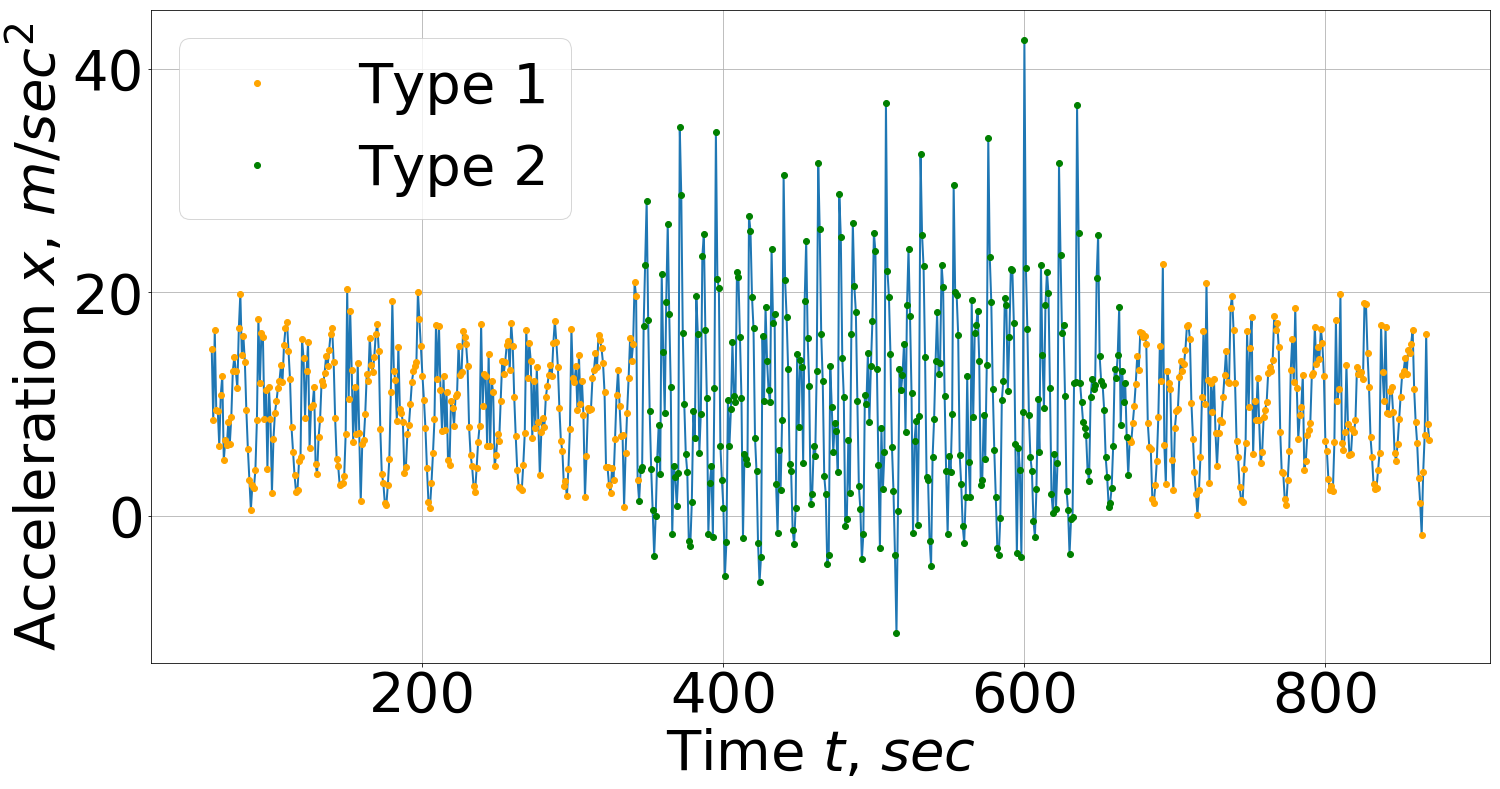
\includegraphics[width=0.5\textwidth]{results/1_real_claster_vector}}
\subfloat[Physical Motion 2]
{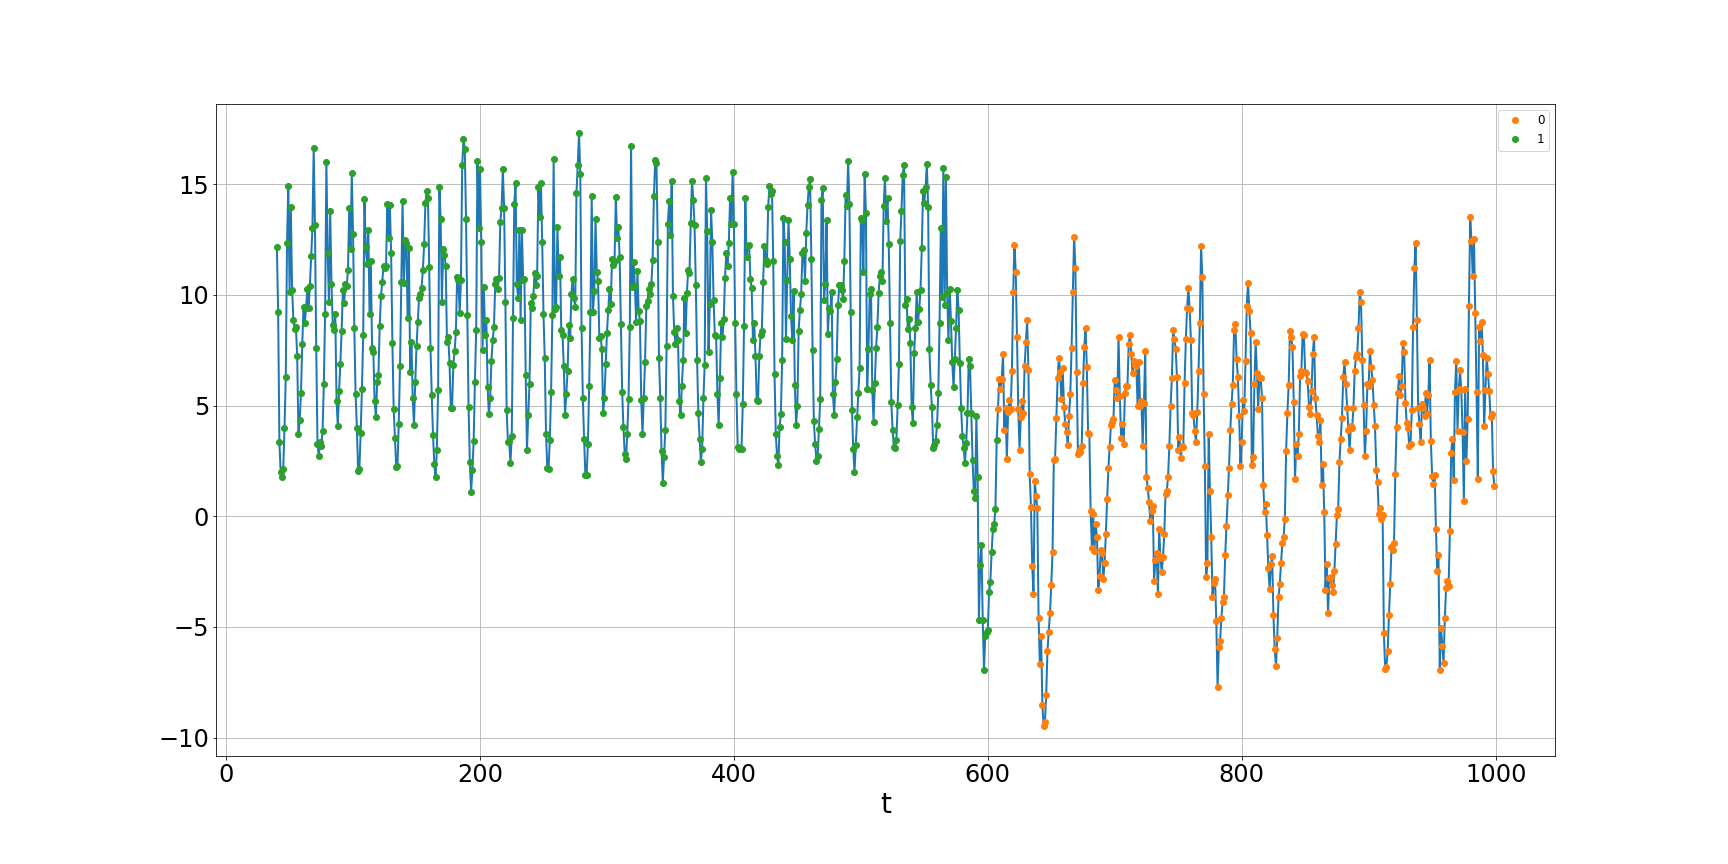
\includegraphics[width=0.5\textwidth]{results/2_real_claster_vector}}\\
\caption{Кластеризация точек временного ряда}
\label{fig_real_claster}
\end{figure}

\begin{table}[h]
\begin{center}
\caption{Результаты работы алгоритма}
\label{table_2}
\begin{tabular}{|c|c|c|c|c|}
\hline
	Ряд & $N$& $K$& $T$& $S$\\
	\hline
	\multicolumn{1}{|l|}{Physical Motion 1}
	& 900& 2& 30& 0.06\\
	\hline
	\multicolumn{1}{|l|}{Physical Motion 2}
	& 1000& 2& 30& 0.03\\
	\hline
	\multicolumn{1}{|l|}{Synthetic 1}
	& 2000& 2& 20& 0.04\\
	\hline
	\multicolumn{1}{|l|}{Synthetic 2}
	& 2000& 3& 20& 0.03\\
\hline

\end{tabular}
\end{center}
\end{table}

\section{Заключение}
В работе рассматривалась задача поиска характерных периодических структур внутри временного ряда. Рассматривался метод основаный на локальном снижение размерности фазового пространства. Был предложен алгоритм поиска характерных сигналов, который основывается на методе главных компонент для локального снижения размерности, а также на использовании некоторой функции расстояния между локальными базисами в каждый момент времени, которые интерпретировались как признакового описание точки временного ряда.

В ходе эксперимента, на реальных показаниях акселерометра, а также на синтетических данных, было показано, что предложенный метод измерение расстояния между базисами хорошо разделяет точки которые принадлежат различным классам, что приводит к хорошей кластеризации объектов. Результаты работы, показаны в таблице~\ref{table_2}.

Предложеный метод имеет ряд недостаткров связаных с большим количеством ограничей на временной ряд. Данные ограничения будут ослаблены в последнующих работах.

\begin{thebibliography}{99}
	\bibitem{cinar2018}
	\textit{Y. G. Cinar and H. Mirisaee} Period-aware content attention RNNs for time series forecasting with missing values~// Neurocomputing, 2018. Vol. 312. P. 177--186.
	
	\bibitem{Ivkin2015}
	\textit{И. П. Ивкин,  М. П. Кузнецов} Алгоритм классификации временных рядов акселерометра по комбинированному признаковому описанию.~// Машинное обучение и анализ данных, 2015.
	
	\bibitem{Katrutsa2015}
	\textit{V. V. Strijov, A. M. Katrutsa} Stresstes procedures for features selection algorithms.~// Schemometrics and Intelligent Laboratory System, 2015.
	
	\bibitem{Borg2005}
	\textit{I. Borg, P. J. F. Groenen} Modern Multidimensional Scaling. --- New York: Springer, 2005. 540 p.
	
	\bibitem{Kanungo2000}
	\textit{T. Kanungo, D. M. Mount et al} An Efficient k-Means Clustering Algorithm: Analysis and Implementation. 2000.
	
	\bibitem{Shiglavsi1997}
	\textit{Д. Л. Данилова, А. А. Жигловский} Главные компоненты временных рядов: метод "Гусеница". --- Санкт-Петербурскиий университет, 1997.
	
	\bibitem{Ignatov2015}
	\textit{A. D. Ignatov, V. V. Strijov} Human activity recognition using quasiperiodic time series collected from a single tri-axial accelerometer.~// Multimedial Tools and Applications, 2015.
	
	\bibitem{Olivares2012}
	\textit{A. Olivares, J. Ramirez, J. M. Gorris, G. Olivares, M. Damas} Detec- tion of (in)activity periods in human body motion using inertial sensors: A comparative study.~// Sensors, 12(5):5791–5814, 2012.

	
\end{thebibliography}

\end{document}

